\documentclass{aa}


% \usepackage[draft]{graphicx}
\usepackage{amsmath}
\usepackage{hyperref}
\usepackage{xcolor}


\title{Palomar 5 Gaps}

\subtitle{Globular clusters as hole punchers}

\author{S. Ferrone
       \inst{1,2}
       \and
       P. Di Matteo\inst{2}
       \and
       M. Montuori\inst{1}
       \and
       A. Mastrobuono-Battisti
       }

\institute{Dipartimento di Fisica, Universit\`a di Roma ``La Sapienza'',
           Piazza Aldo Moro\\
           \email{salvatore.ferrone@uniroma1.it}
      \and
          Paris Observatory. Paris Sciences et Lettres\\
          \email{c.ptolemy@hipparch.uheaven.space}
          \thanks{The university of heaven temporarily does not
                  accept e-mails}
          }

\date{Born in 1996; Accepted in 2018}

\definecolor{darkgreen}{rgb}{0.0, 0.5, 0.0}


\newcommand{\paola}[1]{\textcolor{magenta}{{#1}}}
\newcommand{\salvatore}[1]{\textcolor{darkgreen}{{#1}}}
\newcommand{\marcook}[1]{\textcolor{green}{{#1}}}
\newcommand{\marcoko}[1]{\textcolor{red}{{#1}}}
\newcommand{\qmar}[1]{\textcolor{brown}{{#1}}}



\begin{document}




\abstract
  {Holy moly artichokey}
 % aims heading (mandatory)
  {ok}
 % methods heading (mandatory)
  {good}
 % results heading (mandatory)
  {alright}
 % conclusions heading (optional), leave it empty if necessary
  {done}


\maketitle
\section{Introduction}


  Over a century ago, \citet{1933AcHPh...6..110Z} postulated the existence of dark matter to explain the excessively large velocity dispersions of galaxies within their galaxy clusters. Since then, mounting evidence has been assembled to support this claim. \citet{1970IAUS...38..351F,1970ApJ...161..802F} elaborated on the dynamics of disk galaxies and briefly acknoledged in the appendix of his paper that the rotation curves of NGC 300 and M~33 cannot be fully explained by disk models and that there must be the same amount of mass or more that is undetected and beyond the extend of the galaxies to explain their rotation curves. Concurrently \citet{1970ApJ...159..379R} studied the rotation of Andromenda and observed it to be flat and not decreasing as one would expect from a potential with more mass concentration in the center. Eventually, astronomers returned to Zwicky's non-luminous matter to explain these fast-rotating disks, as discussed in \citet{1983SciAm.248f..96R}'s review. \salvatore{I see why we cite freeman70 now. there are two comments in the appendix stating that there is as much mass beyond the optical limit as there is within it for two different galaxoes. NGC 300 and M 33. It's not clear to me why we cite Rubin 70. The rotation curve is flat, to me implies a logarithmic potential and hence we need dark matter. However, I don't get any impression of missing matter when I read the text.}


  Beyond the galactic scale, dark matter is essential for explaining many cosmological phenomena. For instance, the Planck mission \citep{2020A&A...641A...1P} was designed to study the Cosmic Microwave Background (CMB), whose spectrum closely follows that of a black body with a peak temperature in the millimeter wavelength range, corresponding to approximately 2.725~K. However, there are slight temperature variations on the order of one part in ten thousand. Notably, the colder regions of the CMB temperature map correlate with whole-sky gravitational lensing maps \citep{2020A&A...641A...8P}--since the photons lost energy as they escaped the gravitational wells. The $\Lambda$ Cold Dark Matter ($\Lambda$-CDM) model accounts for these observations almost perfectly, proposing that dark matter exists and that its distribution originated from stochastic quantum fluctuations within the first second of the universe led to density variations. These variations propagated as the universe expanded, shaping the large-scale structure and distribution of galaxies we observe today.


  As laid out in \citet{2021PrPNP.11903865A}'s review, despite significant progress, the true nature of dark matter remains elusive and scientists continue to search for evidence of its existence beyond its gravitational effects on cosmic and galactic scales. A key focus today is detecting dark matter on sub-galactic scales, because at these scales different cosmological scenarios predict different lumpiness of the halos. For instance, \citet{2008ApJ...679.1260M} computed cosmological simulations and compared the Via Lactea simulations \citep{2008ApJ...679.1260M} and demonstrated (\salvatore{I don't quite understand Madau 2008. The main result is that based on the assumptions you can produce a variance in the number of subhaloes that are consistent with global properties of a milky-way like galaxy? I need to discuss this with another human}). \citet{2019Galax...7...81Z} provides a review for the different proposed mechanisms of forming dark matter haloes from perturbation theory and deviations from a uniformly dense medium and also disccses techniques and limitations for modelign such physical phenomena. \citet{2019Galax...7...81Z} rightly states that until particles are discovered $\Lambda$-CDM remains a hypothesis. Since the true nature of dark matter is elusive. The possibilities for sub-galactic behaviour and structure of dark matter are vaste. However, as proposed by Carlberg in 2012, a most promising tool to set limits on the number and mass density of the sub-halos, are stellar streams.
  
  Stellar streams, several-kpc long structures formed by the tidal disruption of globular clusters or dwarf galaxies orbiting a host galaxy. They are one of the evidences for the hierarchical nature of the galaxy formation as predicted by the $\Lambda CDM$ model \citep{white91}. These tidal forces arise due to differential gravitational pulls across extended objects, causing stars farther from the galactic center to lag behind while those closer are pulled away. This stretching creates two tidal tails that trace the cluster's orbit, unless in the closest vicinity to the object \citep{2007ApJ...659.1212M}. Numerical predictions of this phenomenon exist since the 1970s \citep[see, for example][]{1975AJ.....80..290K}. These predictions occured well before the first detections which were made by \citet{1995AJ....109.2553G} around some Galactic globular clusters. Interestingly, this work was a nearly contemporary discovery of the Sagittarius stellar stream by \citet{1994Natur.370..194I} which is the closest example of a stream emerging from a dwarf satellite currently interacting with the Milky Way. Subsequent studies\footnote{\citep[see][for more subsequent observation detections of tidal debris, i.e. globular cluster stars beyond the tidal radius.]{1997A&A...320..776L, 2000A&A...356..127T, 2000A&A...359..907L, 2001AAS...19910906S, 2003AJ....126..815L}} extended Grillmair's findings to other globular cluster streams, until the discovery made by \citet{2001ApJ...548L.165O,2002AAS...200.1001O, 2003AJ....126.2385O} of long and thin tails outside the Palomar~5 globular cluster, which were shown to be extended for more than $10^\circ$ degrees in the sky. These early works stimulated a vigorous search for stellar streams in the Galaxy in the following years \citep{2006ApJ...643L..17G, 2006ApJ...637L..29B, 2006ApJ...637L..29B, 2009ApJ...693.1118G}. The review of Bonaca properly asserts that we have envolved into a new area of stellar stream astronomy Gaia astrometric mission \citep{2016A&A...595A...1G}. 
  
  Gaia's characterization of billions of stars in the Milky Way allows us to look for these structures coupling photometry, astrometry and spectroscopy. The development and deployment of the Streamfinder algorithm has led to the detection of about 90 stellar streams in the Milky Way. \citet{2023MNRAS.520.5225M} provides a summary of these streams and tabulates that about 20 are associated to modern day globular clusters. Thus, currently there are about 70 progenitor-less streams and about 145 stream-less clusteres. The solo-streams can be explained by a larger globular cluster population whose memebers have been disolved due to two body relaxation and tidal stripping. For instance, Z Wan 2020(???) reports that the Phenoix stream is dynamically consistent from a globular cluster yet far more metal poor than any cluster ever observed, galactic or otherwise. This implies that the stream is from a completely disolved globular cluster which comes from a population of clusters that have not survived until modern times. 
  
  \citet{2022MNRAS.516.5331M} showed that many very metal poor streams exist in the Milky Way. On the other hand, it is possible that some globular clusters do not loose a significant number of stars to create tidal tails. For instance, \citet{2022A&A...667A.112V} demonstrated that clusters existing in dark matter subhaloes can place the tidal radius far beyond their half mass radii and sheild stars from escape. Another factor is indeed detectability. Additionally, there are mant cluster in the internal regional of the galaxy, a region overwhich \texttt{streamfinder} was not applied since the high stellar density implicates a computational cost that is currently far to expensive. Also, \citet{2018MNRAS.474.2479B} demonstrates that internal dynamics preferentially kicks out small stars first, which have lower luminosities. Earlier escape times places larger distances to the cluster and make detection more difficult. 
  
  
  One of the interests in studying stellar streams, is that they can constrain the gravitational field of their host galaxies, particularly the Milky Way. ompared to the measurement of the HI rotation curve, stellar streams offer the opportunity to investigate the potential of the host galaxy over a wide range of distances, reaching the outermost regions of the halo. For example, \citet{2011MNRAS.417..198V} demonstrated how stellar streams can infer the mass and scale parameters of dark matter haloes using various amounts of observational data, from basic right ascension and declination to full six-dimensional phase space information. \citet{2018ApJ...867..101B} reviewed this concept from an information-theoretic point of view, identifying which orbits and configurations of stellar streams that yield the most information about the galactic potential. However, the use of single streams for constraining the Galactic potential has led, however, to some ambiguous and not converging results over time. For example, \citet{2010ApJ...718.1128L} made use of the Sagittarius stream to infer that the dark matter halo of our Galaxy has a triaxial shape \citep[but see also][]{2004MNRAS.351..643H, johnston05, 2005ApJ...619..807L}; \citet{2016ApJ...833...31B} concluded that the dark matter halo of our Galaxy is nearly spherical at the radii of the Palomar~5 and GD~1 streams. Nonetheless, a recent goal of stellar stream astronomy was realized by \citet{2024ApJ...967...89I} constructed the most accurate model of the Milky Way to date based on a set of about 90 streams. 

  In this study, we build on this body of work by investigating another important use case for stellar streams: probing dark matter on sub-galactic scales. According to simulations by Springel et al. (2008), $\Lambda$-Cold Dark Matter ($\Lambda$CDM) predicts that galaxies grow hierarchically, with dark matter clumps forming at a wide range of masses and sizes. These clumps, or \textit{subhalos}, are predicted to follow a mass distribution with a power-law slope slightly shallower than -2.0. To date, the smallest observed dark matter halo was detected through gravitational lensing in an Einstein ring and had a mass of $10^8$ solar masses, as described by \citet{2012Natur.481..341V}. However, some models predict that dark matter clumps could exist down to the mass of Earth-like planets at least \citep[see][ and discussion in \citet{2021arXiv211101148A}]{2005JCAP...08..003G, wang20}. 

  \citet{2002MNRAS.332..915I} first suggested that dark matter subhalos could influence stellar streams by diffusing their orbital elements. Later, \citet{2012ApJ...748...20C} expanded this idea, proposing that subhalos could create gaps in stellar streams during flyby encounters, where a subhalo approaches closely enough to a segment of a stream and significantly changes the orbits of the closest stars. Carlberg 2013 further explored this idea through a probabilistic model of encounter rates based on the expected subhalo distribution. \citet{2019ApJ...880...38B} provided observational evidence for this idea, identifying an underdensity in the GD-1 stream that could not be explained by known objects, such as globular clusters, and, interestingly enough, was inconsistent with the $\Lambda$CDM mass-size relationship presented in \cite{2017MNRAS.466.4974M}.

  Our study focuses on the influence of globular clusters on stellar streams, specifically examining whether globular clusters could produce gaps similar to those expected from dark matter subhalos. If globular clusters do indeed create such gaps, this factor must be considered when using stellar streams to detect dark matter. An additional and unique aspect of our study is that we focus on modeling real stellar streams. We focus on the Palomar 5 stream, which is well-studied, has observable gaps \citep{2020ApJ...889...70B}, and is highly visible due to its position above the galactic disk. We present a result from one of our simulations in Fig.~\ref{fig:stream_on_sky}, and the following sections describe our modeling of the stream, the gravitational interactions with the galaxy and other globular clusters, and the statistical analysis of perturbations affecting the stream.


  \begin{figure*}
    \centering
    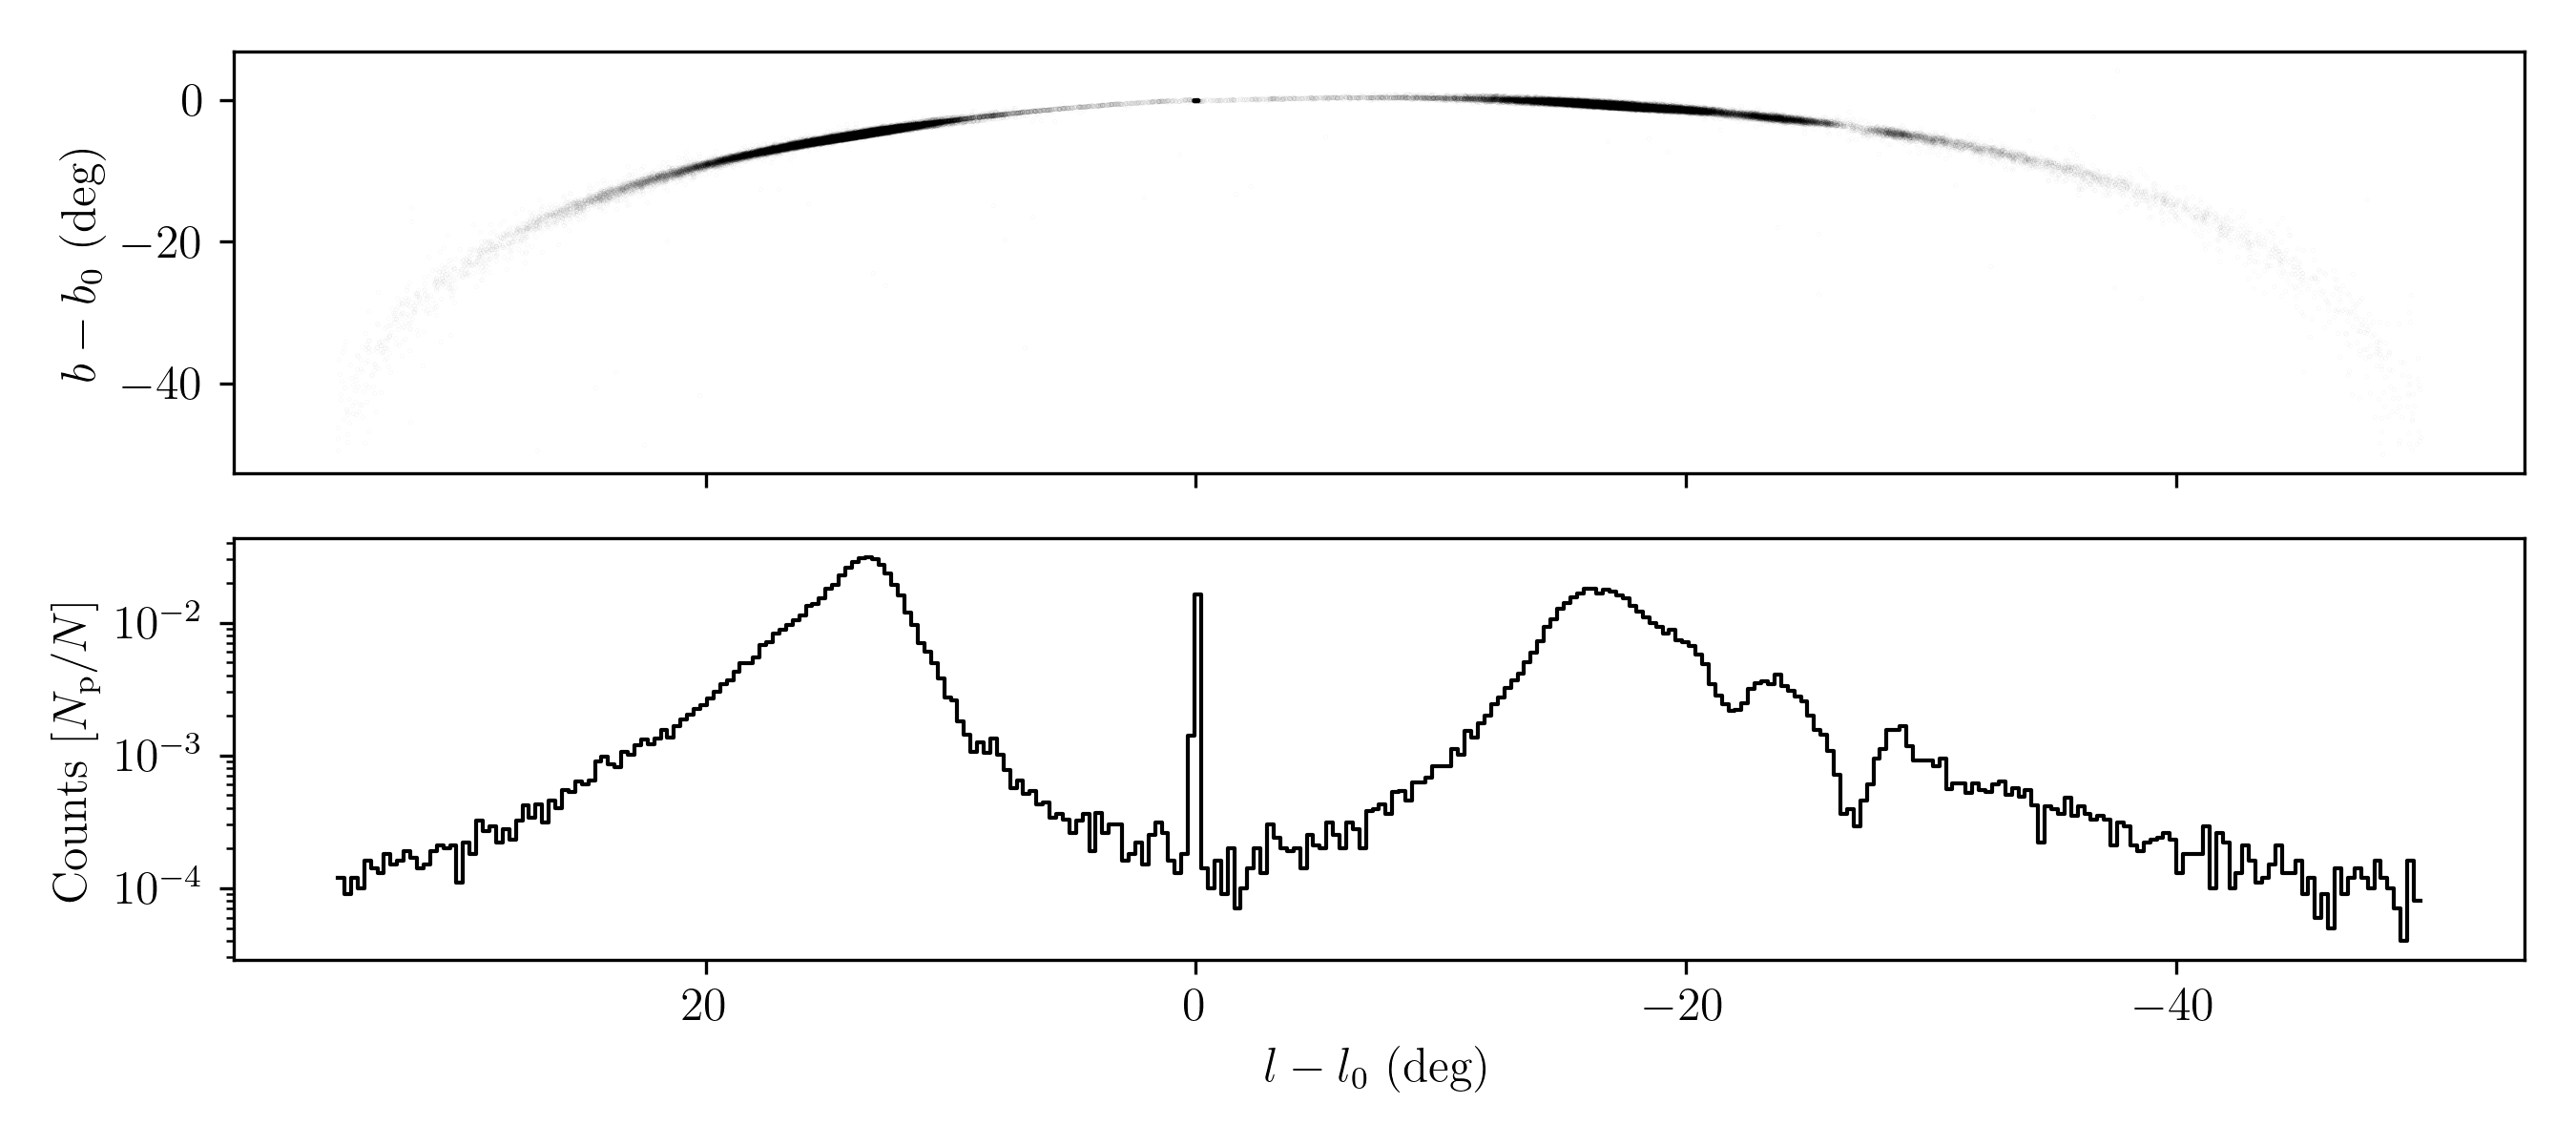
\includegraphics[width=\linewidth]{stream_on_sky_Pal5_monte-carlo-009_pouliasis2017pii-GCNBody.png}
    \caption{An instsance of the Palomar 5 stream created modeling the cluster as a plummer sphere within an axis-symmetric galactic potential plus 164 other galactic globular clusters. The top plot is a scatter plot of star-particles that escaped the cluster due to tidal forces, the bottom plot shows the marginalized 1D density profile in longitude. Two large gaps are present and are due to the passage of two globular clusters.}
    \label{fig:stream_on_sky}
    \end{figure*}








\section{Methods}

  \subsection{Numerical Methodology}
    Our numerical methodology follows the approach outlined in Ferrone et al. (2023), which we present here for completeness. We begin by extracting the phase space properties (positions, velocities) as well as the masses and half-mass radii of 165 globular clusters from the galactic globular cluster catalog by \cite{2021MNRAS.505.5957B}.\footnote{The Baumgardt catalog has been assembled across a series of works, see: \cite{2020PASA...37...46B,2019MNRAS.482.5138B,2018MNRAS.478.1520B} as well. The catalog can be found on the World Wide Web at \href{https://people.smp.uq.edu.au/HolgerBaumgardt/globular/}{https://people.smp.uq.edu.au/HolgerBaumgardt/globular/}.} We handle the uncertainties on the measured phase space parameters through a monte-carlo approach. The catalog provides uncertainties for mass, distances, line of sight velocities, proper motions and includes a covariance term between the proper motions---uncertainties for the right ascension, declination, and the characterisitcs radii are not available. We repeate simulation the creation of Palomar 5's tidail tails 50 times, for each of which we vary the initial conditions of each cluster by sampling its five-dimensional gaussian uncertaintiy distribution. For the first simulation, which we name \texttt{Sampling 000}, we use the most probable values for the initial conditions. 

    We convert the initial conditions from sky coordinates into a galactocentric reference frame. We use the local standard of rest and the peculiary motion of the sun as reported by Sch\"onrich 2010. The circular velocity at the solar radius was set to: $v_{\text{LSR}} = 240$~km~s$^{-1}$. The peculiar velocity of the sun was set to $(U_\odot, V_\odot, W_\odot)=(11.1, 12.24, 7.25)$~km~s$^{-1}$. The position of the Sun was set to $(x_\odot,y_\odot,z_\odot) = (-8.34,0,0.027)$~kpc, vertical position above the disk was taken from Chen et al 2001 and the galacto-radial distance was taken from Reid et al 2014. These transformations were performed using \texttt{astropy} \citep{2013A&A...558A..33A}.


    For the galactic potential, we used the second static model from \citet{2017A&A...598A..66P}, a superposition of a thin disk, thick disk, and dark matter halo, with masses and scale lengths provided in Table 1 of \citet{2023A&A...673A..44F}. This model is time-independent throughout our simulations. To balance data volume and computation time, we use only one galactic potential, which should suffice. \citet{2021MNRAS.505.5978V} found that only a few outer globular clusters are strongly affected by different potential models, with kinematic uncertainties being the dominant factor in orbital solution differences. Similarly, \citet{2024MNRAS.528.5189G} generated a globular cluster mass-loss catalog using seven different potential models and found their debris distributions to be model-independent. While the clusters' positions may depend on the model, we assert that interaction rates and stream formation are unaffected by the choice of galactic model.    

    The primary methodological departure from \citet{2023A&A...673A..44F} is that now we include globular cluster interactions. Instead of treating the clusters as point masses that only experience the gravitational potential of the galaxy, we now compute N-body interactions between the clusters during the backward integration over 5 billion years. The equations of motion for the globular cluster system are thus: 
    \begin{equation}
      \ddot{\vec{r}}_i = -\nabla \Phi(R_i,z_i) + \left.\sum_{j\neq i} \frac{Gm_j}{\left(|\vec{r}_j - \vec{r}_i|^2 + b_j^2\right)^{3/2}}\right. \left(\vec{r}_j - \vec{r}_i\right),
    \end{equation}\label{eq:GCNBody} where $\vec{r}$ indicates the galacto-centric position, the index $i$ indicates a globular cluster of interest with $R_i,z_i$ being its galactocentric positions in cylindrical coordinates. The index $j$ indicates the other globular cluster that are summed over where: $m_j$ is its mass, $b_j$ is its plummer scale radius, and $r_j$ is it's galacto-centric position. $\Phi$ is the axis-symmteric potential of the model used for the Milky Way. 

    At their computed positions 5 Gyr ago, each globular cluster was assigned 100,000 particles sampled from a Plummer distribution to represent its stellar content. For each set of initial conditions, the particle positions were resampled to account for uncertainties in mass, which is an improvement from \citet{2023A&A...673A..44F}. Since globular clusters are older than 8 Gyr, their most massive stars have already gone supernova, leaving primarily low-mass stars, typically under one solar mass (\@\salvatore{Citation? Paolo knows this stuff well.}). Given that clusters usually have masses between $10^5-10^6$ solar masses, 100~000 particles is sufficient to represent the distribution of tidal debris.

    
    We then integrated the evolution of these particles forward in time to the present day. During this forward integration, each star particle feels the gravitational influence of the galaxy and all globular clusters, but not other star particles. We do not perform direct N-body simulations between star particles as in eq.~\ref{eq:GCNBody}; instead, at each time step, we load the positions of all globular clusters, as found from the initial integration, and apply their forces to the star particles. The equation of motion is thus: 
    \begin{equation}
      \ddot{\vec{r}}_p = -\nabla \Phi(R_p,z_p) + \left.\sum_{j} \frac{Gm_j}{\left(|\vec{r}_j(t) - \vec{r}_p|^2 + b_j^2\right)^{3/2}}\right. \left(\vec{r}_j(t)- \vec{r}_p\right),
      \end{equation} \label{eq:equation_of_motion_particle} where the index $p$ represents one of the 100,000 particles of interest.

    The integration was performed using a leapfrog integrator. The timestep size was chosen to be based on two critera. First, to ensure the conservation of energy to XXX. The second, is the drift in position due to numerical error over 5 Gyr was negligible compared to the scale radius of the globular clusters, which is about 5~pc. Further details on the timestep selection are discussed in the appendix.

    During the integration, intermediate snapshots were saved to facilitate the analysis of stellar streams and the effects of cluster impacts. Specifically, for each of the 50 realizations of the Palomar 5 stream, we saved $5000$ intermediate timesteps which is a temporal resolution of 1 million years. To provide an estimate of the size of our simulations, we have:
    \begin{tabular}{c|c|c|c}
      $N_p$ & $N_{\textrm{ts}}$ & $N_{\textrm{phase}}$ & $N_{\textrm{sampling}}$  \\
      \hline
      $100000$ & $5000$ & $6$ & $50$   \\
    \end{tabular} 
    where $N_p$  is the number of particles, $N_{\textrm{ts}}$ is the number of time-steps saved, $N_{\textrm{phase}}$ is the number of phase space coordinates, and $N_{\textrm{sampling}}$ is the number of monte-carlo samplings of the initial conditions. Using single precision floating point numbers, the size of our simulations is approximately:
    \begin{equation} \label{eq:data_volume_estimate}
      N_p \times N_{\textrm{ts}}\times N_{\textrm{phase}}\times N_{\textrm{sampling}} \times 4~\textrm{bytes}\approx 600~\textrm{Gb}.
    \end{equation}




  \subsection{Gap Detection and Characterization} \label{sec:gap_methods}

    At the end of the simulations, some gaps in the stellar stream are so prominent that they can be identified visually without any sophisticated quantitative analysis. The analysis of the morphology of the tidal tails of Palomar~5 is carried out by comparing simulations with globular clusters (called \texttt{full}) and without them (called \texttt{reference}). A preliminary evaluation is performed visually, followed by a quantitative analysis of the differences between the density profiles in the two mentioned cases. 


    % We initially sought an automated, quantitative approach from signal and image processing that could reliably detect all gaps and evaluate their significance. Unfortunately, despite extensive efforts, an ideal method remained elusive. As a result, we opted for a simpler approach: a combination of visual inspection aided by comparative analysis.


    The \texttt{reference} simulations used the same 50 sets of initial conditions but excluded interactions with globular clusters, except for the host cluster, Palomar 5. In other words, the gravitational influence of all other clusters on the star particles within the stream was omitted. By comparing the morphological differences between these \texttt{reference} simulations and the \texttt{full} simulations, we could more effectively identify and assess the impact of globular clusters on the stream's structure. Details on gap identification are provided in Appendix~\ref{sec:gap_detection}, and the identification of corresponding perturbing globular clusters is detailed in Appendix~\ref{sec:Perturber_Identification}.


    Comparisons between the \texttt{reference} and \texttt{full} simulations were performed in the tail coordinate system. This system allows for consistent morphological comparisons by aligning the stream with the cluster's orbit. The coordinate system is based on the work of \citet{2004AJ....127.2753D} and is shown in Fig.~\ref{fig:TailCoordinates}. Briefly, the x' coordinate represents the position of a particle along the orbit relative to the globular cluster—whether it is ahead or behind the cluster. The y' coordinate measures the particle's distance within the orbital plane, where positive values indicate that the particle is farther from the Galactic center and negative values indicate that it is closer.

    
    Once the gaps and perturbers were identified, we sought to characterize the properties of the globular clusters that caused gaps and differentiate them from those that did not. \citet{2013ApJ...775...90C} initiated the theory of gap creation in stellar streams due to gravitational flybys. This analysis was extended both analytically and numerically by \citet{2015MNRAS.450.1136E}, who studied uniform-density streams on circular orbits. \citet{2016MNRAS.457.3817S} presented the most comprehensive theory, generalizing Erkal et al.'s work to include impacts on streams of varying densities on inclined and eccentric orbits using an action-angle approach.

    The significance of an impact is measured by the change in momentum imparted to the stream stars by the perturber. A useful approximation for the change in momentum is the force at the closest approach multiplied by an estimate of the interaction time: \begin{equation} \label{eq:change_in_momentum} \Delta v \approx \text{Force} \times \text{interaction time} = \frac{GM}{b^2} \times 2\frac{b}{v} = 2\frac{GM}{bv}, \end{equation} where $M$ is the mass of the perturber, $b$ is the impact parameter, $v$ is the relative velocity of the perturber with respect to the particle, and $G$ is the gravitational constant. We compute this for the five closest approaches of all globular clusters throughout each of the 50 simulations. Details on how this computation was performed are given in Appendix~\ref{sec:reconstruction}. Ultimately, we obtained a sample of 250 impacts and compared the impact geometry of those that caused gaps with those that did not.
    

\section{Results}



  \subsection*{Overview}

    \begin{figure*}
      \centering
      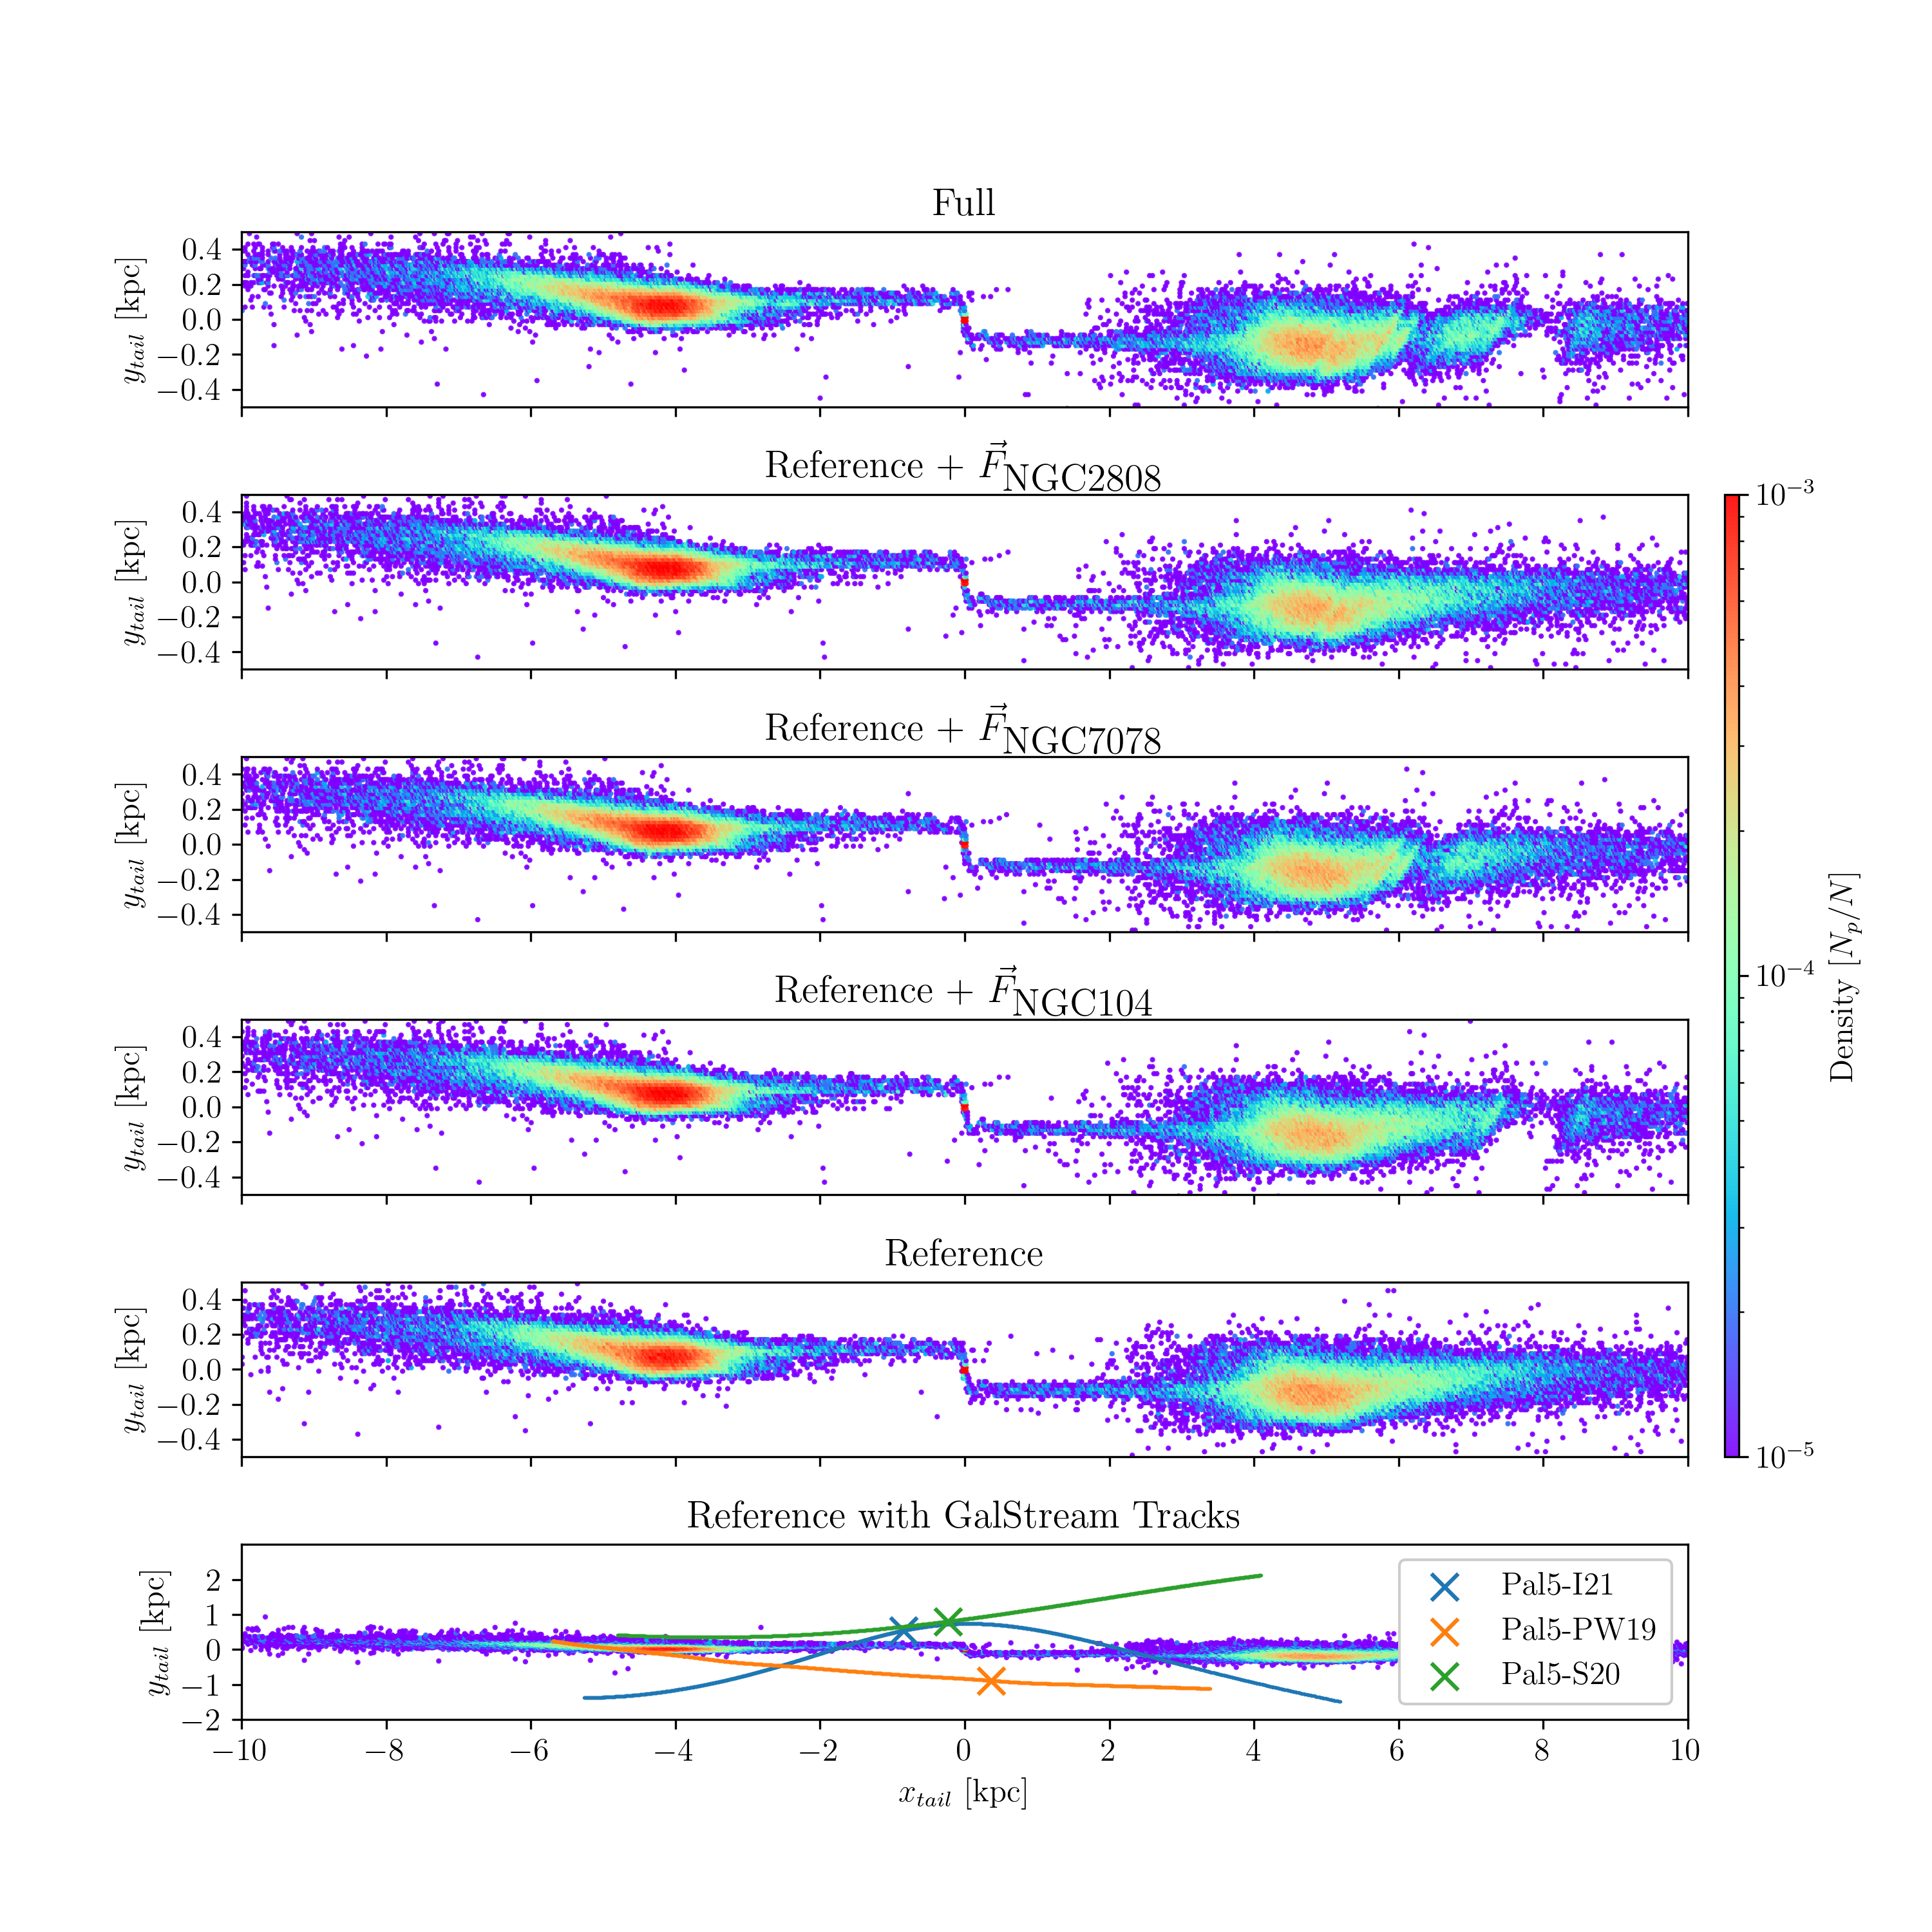
\includegraphics[width=\linewidth]{decomposition-monte-carlo-009-with-3-gaps.png}
      \caption{This figure decomposes the gaps shown in the middle panel of Fig.~\ref{fig:profiles} into the individual perturbuers whose cause them, as identified from Fig.~\ref{fig:force-on-orbit}. These simulations only include the suspected globular clusters in one-at-a-time.}
      \label{fig:decomposition}
    \end{figure*} 

    To our knowledge, this is the first study to investigate interactions between globular clusters in this context. We included N-body forces on the orbits with the globular clusters, yet did not observe significant changes to orbital properties, such as energy or angular momentum, between any of the globular clusters in any simulation. This result is expected given the small sizes and vast distances between the clusters.

    We inspected all simulations upon their completion and present one particularly clear example shown in Fig.~\ref{fig:stream_on_sky} which we selected for its prominent gaps. Two of these gaps are visible in galactic coordinates and become even more apparent when marginalizing over latitude to view their 1D density profile over longitude.
    

    We applied the gap detection methods described in Appendix~\ref{sec:gap_detection}, along with the perturber identification methods from Appendix~\ref{sec:Perturber_Identification}. Results from all simulations are presented in Appendix~\ref{sec:gallery_of_gaps}. Once we identified the perturbers responsible for each gap, we conducted additional simulations to verify correct identification of the perturbers. These additional contain only the suspected clusters and were launched one-at-a-time to isolate the effects of a specific clusters. These results are shown in Fig.~\ref{fig:decomposition}. A summary of which perturber caused a gap and when is presented in Fig.~\ref{fig:histogram_impact_time}. 

    \begin{figure*}
      \centering
      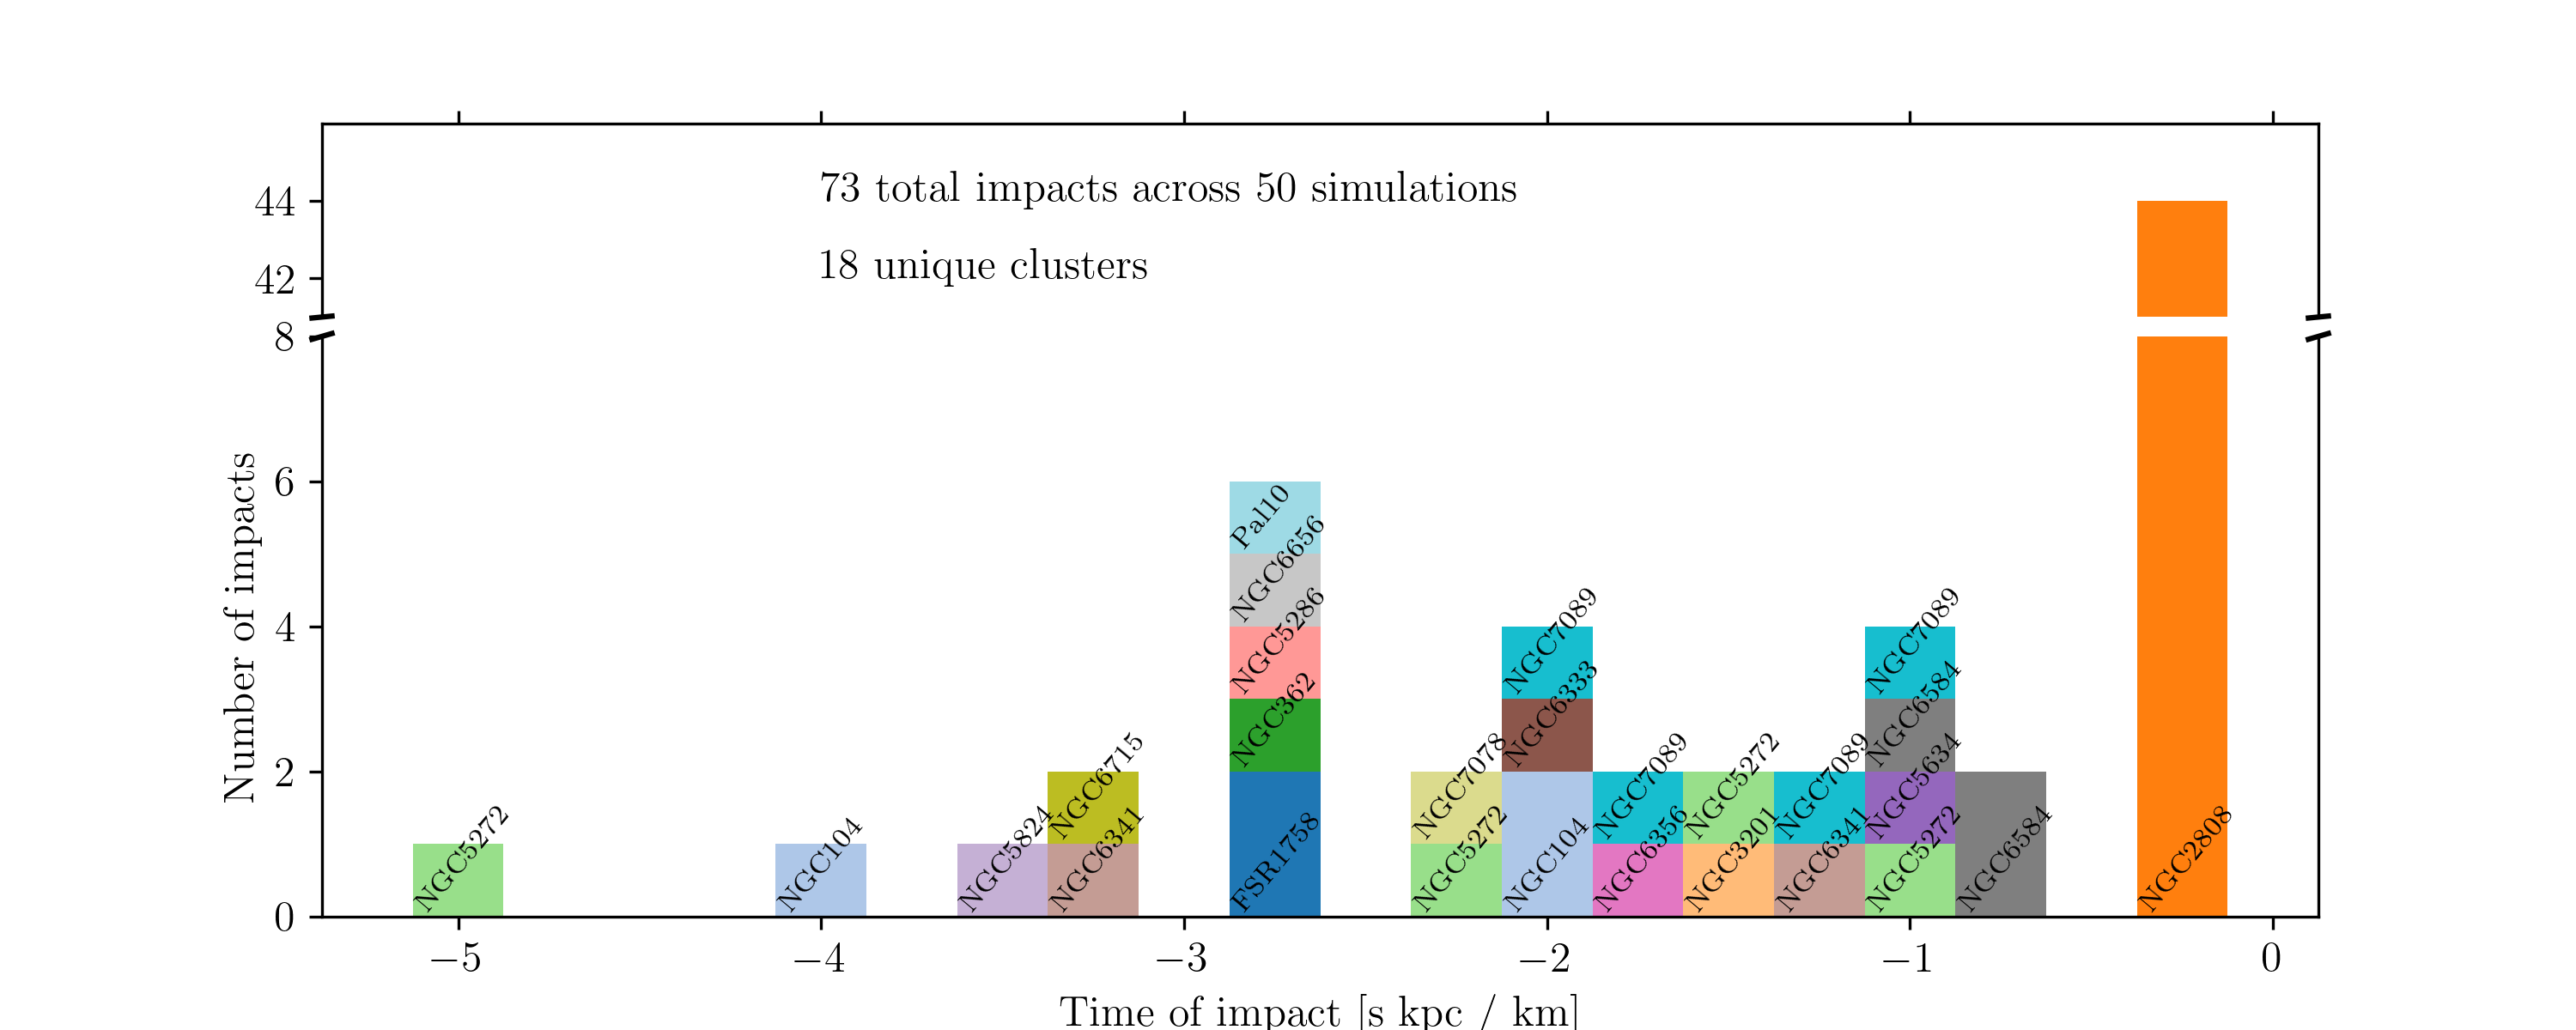
\includegraphics[width=\linewidth]{histogram_impact_time.png}
      \caption{The time of impact for all gap causing flybys summed over all 50 simulations. Each perturbing cluster is label and is color consistent. The time axis is given in simulation units, with 1~s~kpc~km~$^{-1}$ corresponding to roughly 1~Gyr. Note that the y-axis is broken to accommodate the large number of encounters from NGC2808, without overshadowing the other interactions.}
      \label{fig:histogram_impact_time}
      \end{figure*}



    NGC~2808 impacts Palomar 5's stream about 200 Myr ago in 44 out of 50 simulations, creating a small gap at a similar position in each case. The gap size aligns with gap formation as a dispersion process, where stars gradually spread apart due to slight differences in orbital frequencies. Smaller gaps indicate more recent encounters. Since this interaction occurred less than one orbital period ago, the orbital solutions remain similar, producing consistent results across simulations.


    Most gaps appear in the leading tail, which we consider coincidental, as stars escape the cluster's L1 and L2 points at similar rates, and the small distance difference between tails' galactocentric distance is negligible. We expect gaps to be equally likely in both tails. However, only 8 of the 73 gaps occur in the trailing tail, with 44 linked to NGC2808's flyby. After removing these, there are 21 gaps in the leading tail and 8 in the trailing. By the binomial distribution, the probability of observing up to 8 successes in 29 trials, given a 50\% chance of success, is 1.2\%—unlikely, but possible. Additionally, other perturbers impact at consistent times, which may also violate the assumption of independent events, as seen with NGC2808.




    Overall, across 50 simulations, we observe 73 gaps. The distribution of simulations with a given number of gaps is as follows: \begin{tabular}{|l|c|c|c|c|c|}
      \hline
      Number of Gaps & 0 & 1 & 2 & 3 & 4 \\
      \hline
      Number of Sims. & 4 & 25 & 16 & 4 & 1 \\
      \hline
    \end{tabular} Excluding NGC~2808, we are left with 29 gaps, leading to an expected range of 0.6-1.5 gaps per simulation.

    



 
 \subsection*{Perturber Statistics}
  

    We aim to identify general characteristics of perturbers that distinguish them from globular clusters that do not affect the Palomar 5 stream. Fig.~\ref{fig:mass_size_plane} presents several analyses to explore this.

    
    \begin{figure*}
      \centering
      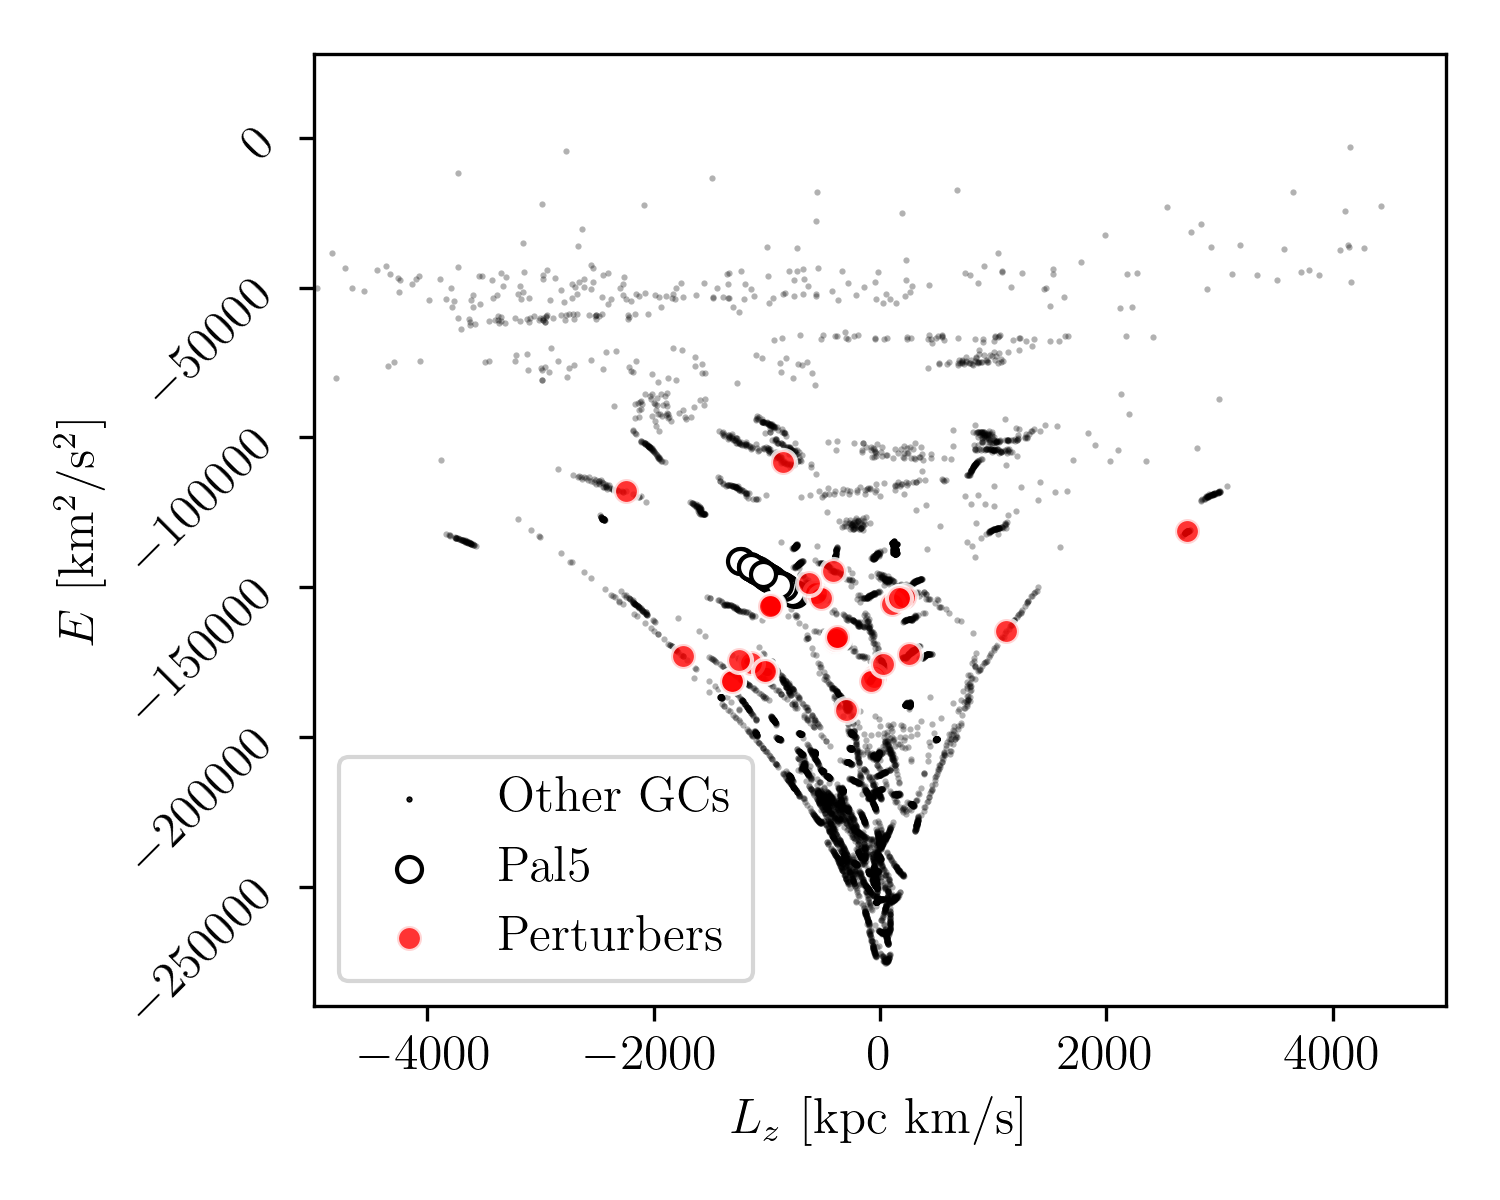
\includegraphics[width=0.45\linewidth]{E_Lz_perturbers.png}
      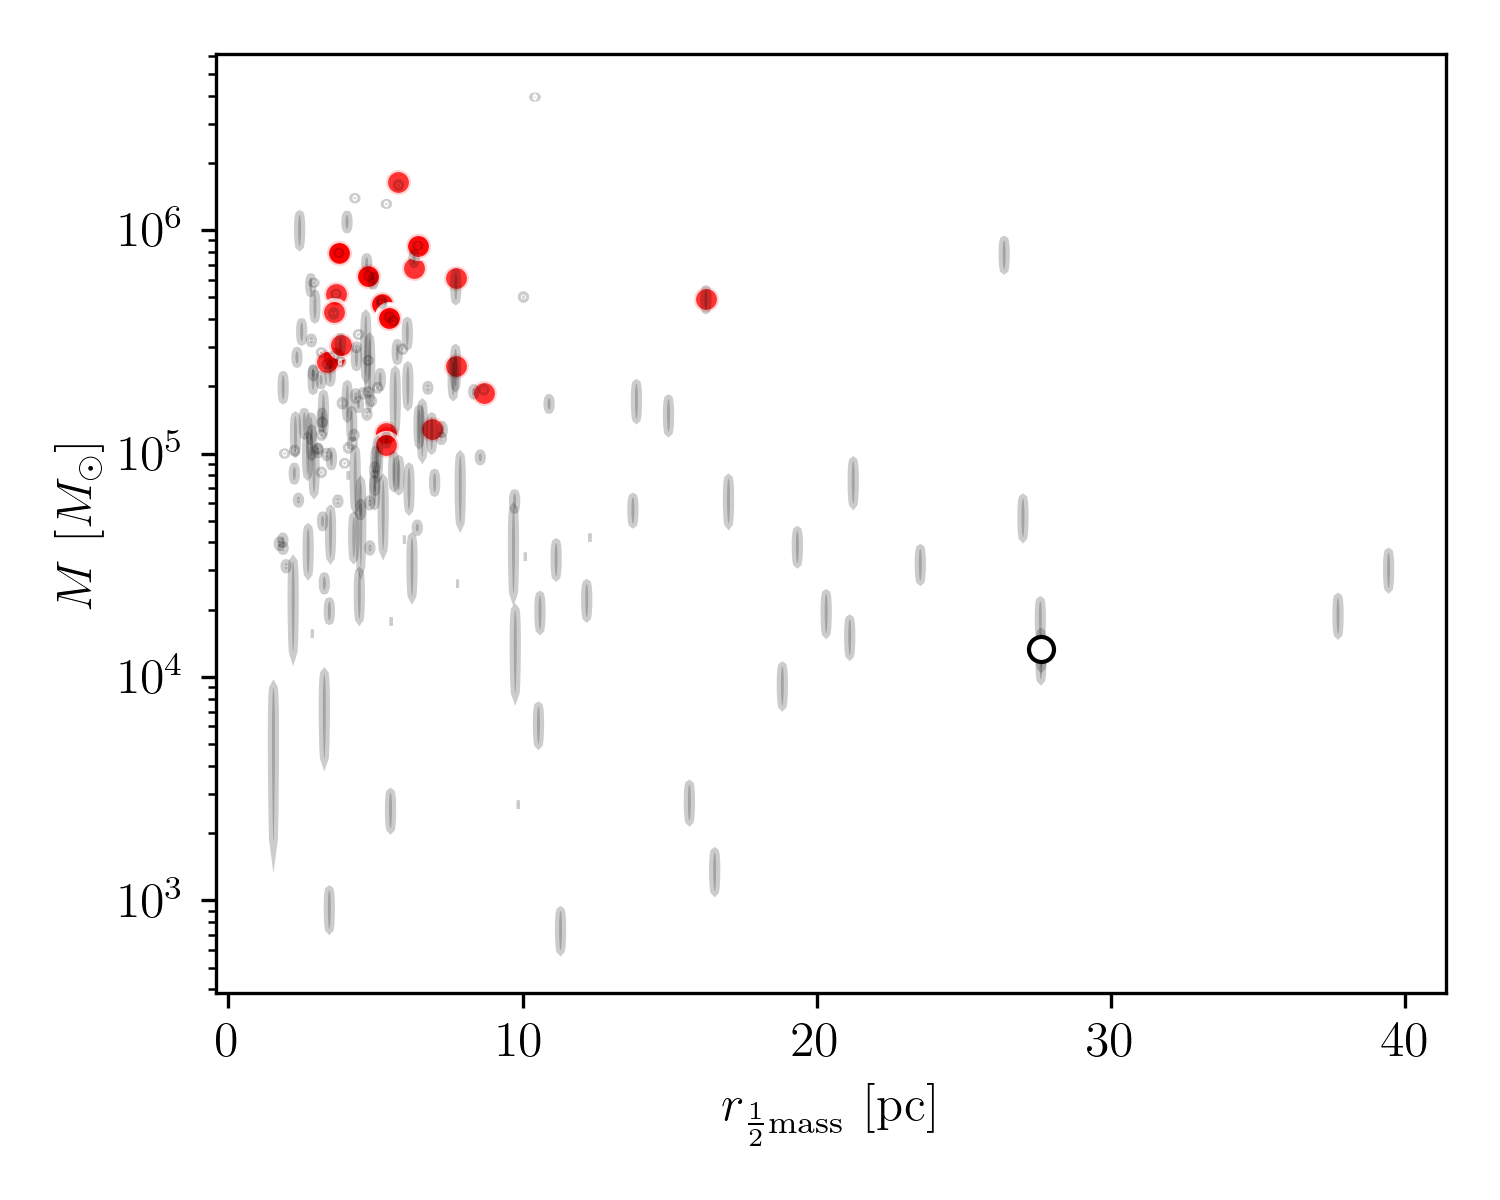
\includegraphics[width=0.45\linewidth]{mass_size_plane.png}

      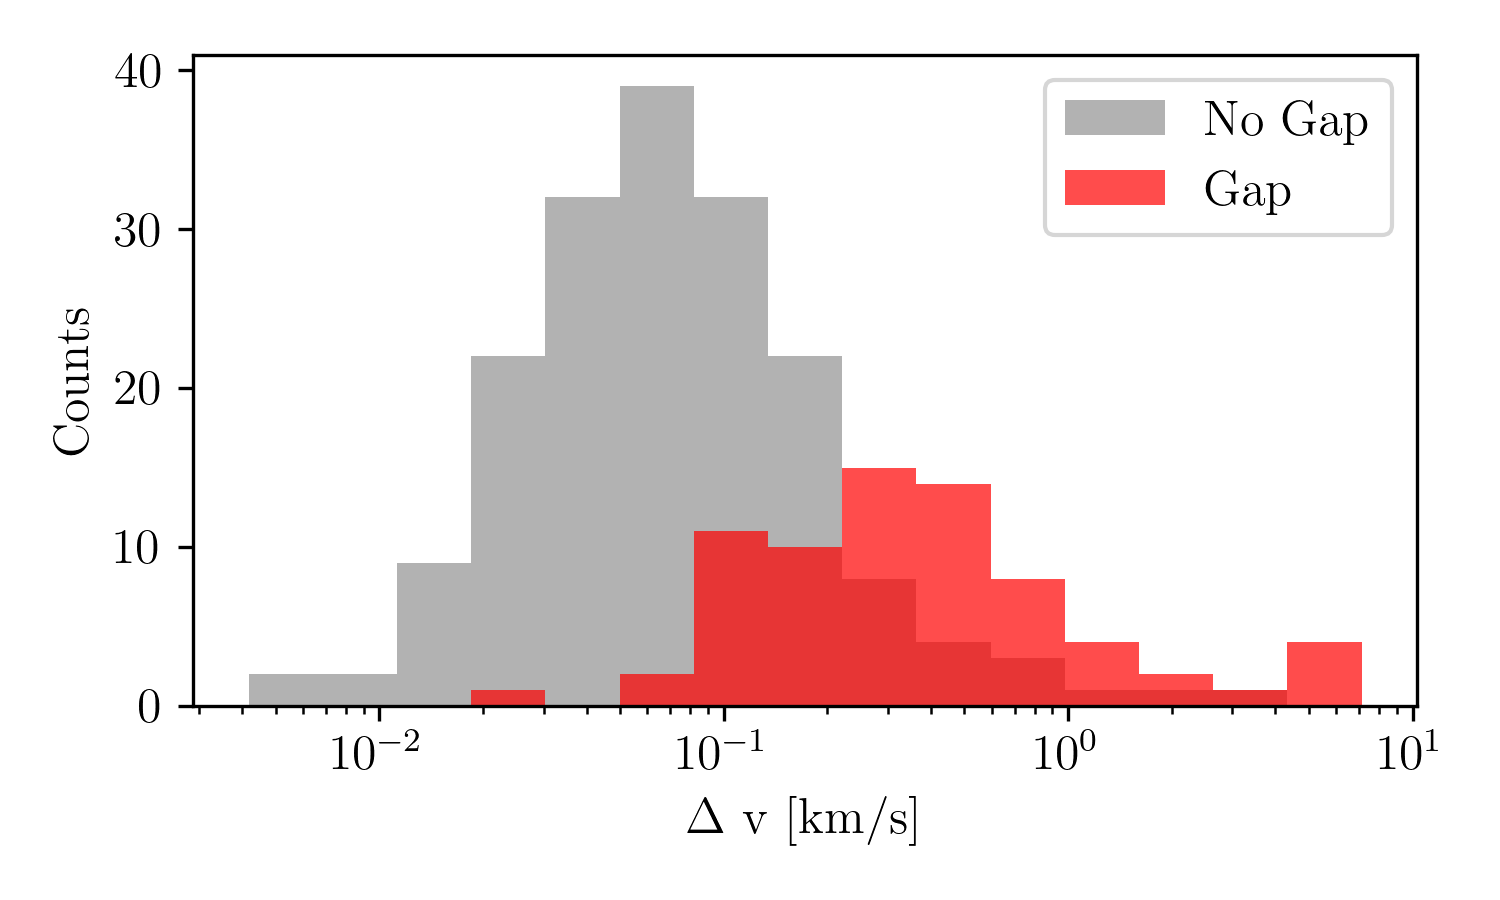
\includegraphics[width=0.45\linewidth]{impact_geometry_statistics_deltaP.png}
      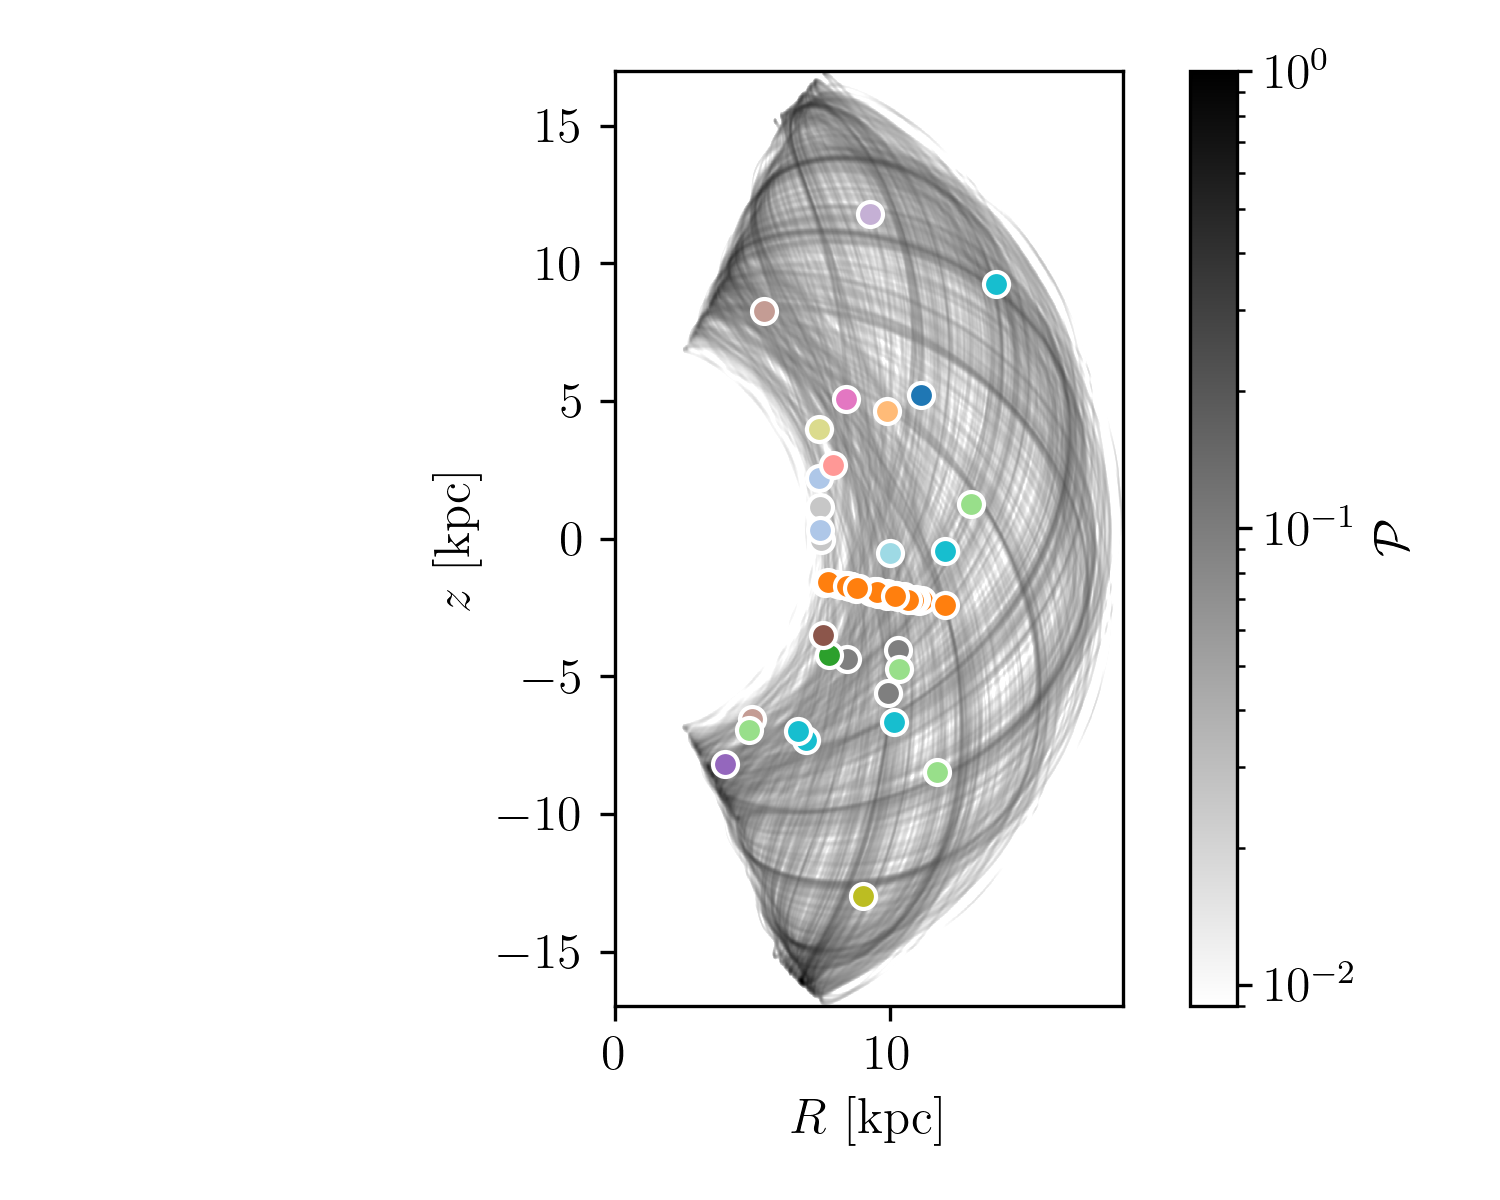
\includegraphics[width=0.45\linewidth]{impact_stats_phase_space.png}
      \caption{\textbf{Characterisitcs of gap causing clusters}--\textit{Note} that the colors of the markers and histogram bars are consistent with Fig.~\ref{fig:histogram_impact_time}.\\ \textbf{Top Left:} Energy-angular momentum space of the globular clusters in the simulations, with 50~$\times$~165 data points representing all sampled initial conditions. Clusters impacting Palomar 5 are shown with colored markers; non-gap-causing clusters are gray. Palomar 5 is marked with a white symbol and black edge. The circular velocity-curve is drawn with a light-pink dashed curve.\\ \textbf{Top Right:} The mass-size plane. Uncertainties on the mass are indicated with vertical bars. \\ \textbf{Bottom Left:} The distribution of imparted momentum from a cluster flyby given by Eq.~\ref{eq:change_in_momentum}. The data set includes the top 5 strongest flybys from each simulation. Those that cause gaps are colored while those that do not are left in black. \\ \textbf{Bottom Right:} Palomar 5's orbit in the meridional plane. The grayscale represents all 50 stacked orbits, with $\mathcal{P}$ indicating the probability of  Palomar~5's position, normalized to $\mathcal{P}_\textrm{max}=1$. Markers show the perturber's position during each impact.}
      \label{fig:mass_size_plane}
      \end{figure*}

      The top-left panel shows that all clusters impacting the stream fall within a specific range of orbital energies, between $-2$ and $-1 \times10^5~\textrm{km}^2\textrm{s}^{-2}$. This is expected, as only clusters within Palomar 5's orbital space can interact with the stream. Our results are consistent with the findings from \citet{2021MNRAS.505.5978V}, who identified a wide range of orbital solutions for the least bound clusters, including both retrograde and prograde orbits. In our potential model, only three clusters samplings had positive orbital energies.
    

      The mass-size relation, shown in the top-right panel, reveals a lower limit of $10^5~\textrm{M}_{\odot}$ for clusters that provoke gaps. While mass and size alone are insufficient predictors, this empirical limit is useful because relative velocity and impact parameters are historical values. The bottom-left panel offers a more physically meaningful result: gap-creating impacts tend to impart more momentum into the stream than non-gap impacts, though with some overlap. While \citet{2015MNRAS.450.1136E} extended the three-parameter model (Eq.~\ref{eq:change_in_momentum}) to include the size of the perturber and the perpendicular and parallel components of relative velocity, we found no clear combination of these factors that distinguishes gap from non-gap cases.
    
      Further insights are shown in Fig.\ref{fig:impact_geometry_statistics}, highlighting a maximum impact parameter of around 200~pc, roughly the width of the stream. Additionally, as \citet{2016MNRAS.457.3817S} demonstrated, the dispersion of action-frequencies in the stream plays a role. Regions of the stream with well-separated frequencies are more susceptible to gap formation, while those with a wide frequency range (near the cluster) tend to erase the history of impacts. Thus, for a gap to form, the imparted change in frequency must exceed the range of frequencies in the impacted region. Thus, the strong flybys that occured close to the cluster and were thus inconsequential for gap formation.


      The bottom-right panel reveals a strong negative correlation between the location of impacts and the galactocentric radius, $r$. The number of gap creating impacts follows the relation $N = -2.5r + 50$, with a Pearson coefficient of -0.86. This is a non-obvious result. While there are more clusters near the galactic center, orbits naturally spend more time near their apocenters, and the lower relative velocities in these regions should favor gap creation. However, this result suggests that cluster galactic number density outweighs these factors in determining the number of gaps.


      Lastly, \citet{2012ApJ...748...20C} conceptualized the number of gaps using a statistical quantity: the rate at which gaps are created per unit stream length. For our simulations, this is given by: \begin{equation} \label{eq:gap_creation_rate}
      \mathcal{R}_{\textrm{Pal 5}} =  \frac{1}{T}\int_{0}^T l^{-1}(t) \sum_i \delta(t-t_i) dt,\end{equation}where $T$ is the total integration time, $l(t)$ is the length of the stream, and $\sum_i \delta(t-t_i)$ sums over the gap occurrences, with $i$ indexing over the number of gaps in a given simulation. Here, $\delta$ represents the diract delta function. This expression can be simplified to:\begin{equation}\mathcal{R}_{\textrm{Pal 5}} =  \frac{1}{T} \sum_i \frac{1}{l (t_i)}. \end{equation}
      This computation allows us to analyze the distribution of gap creation rates across all simulations. The results are shown in Fig.~\ref{fig:TailCoordinates}. This is roughly consistent with a simple estimate of the average gap creation rate: with 72 gaps over 5 Gyr of integration time for a stream about 20 kpc in length, the naive estimate is approximately 0.014~[km~s$^{-1}$~kpc$^{-2}$]. This is about double the weighted mean gap creation rate of 0.009~[km~s$^{-1}$~kpc$^{-2}$]. The naive estimate is higher because it does not account for the growth of the stream over time, unlike Eq.\ref{eq:gap_creation_rate}, where the likelihood of impacting a shorter stream is lower.

      \begin{figure}
        \centering
        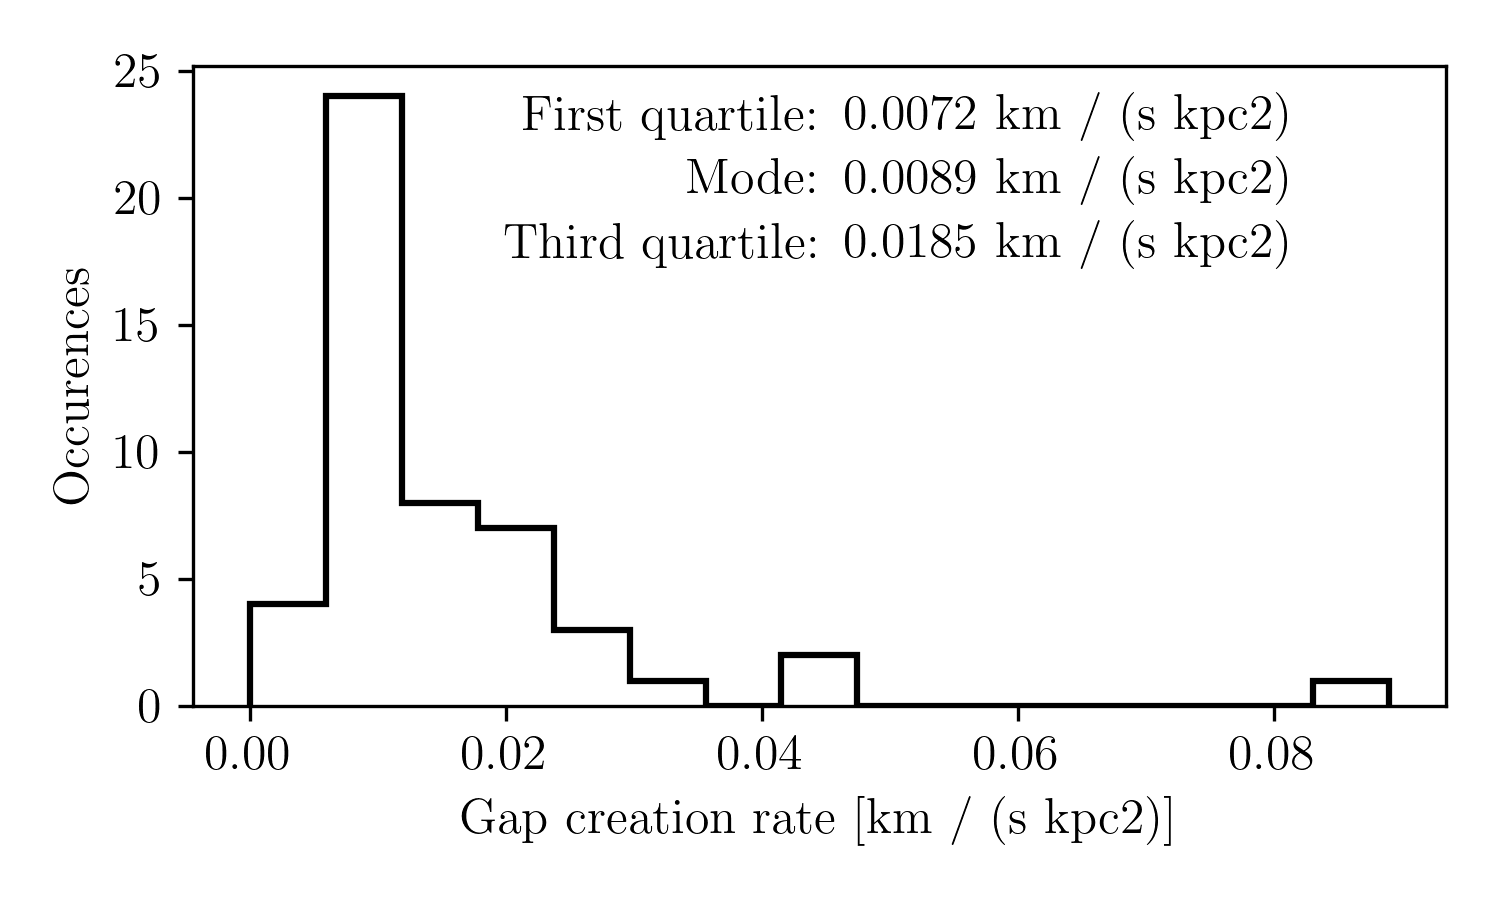
\includegraphics[width=\linewidth]{gap_creation_rate.png}
        \caption{The distribution of the number of gaps normalized over the total integration time and unit stream length, as described by Eq.\ref{eq:gap_creation_rate}. }
        \label{fig:TailCoordinates}
      \end{figure}
      




\section{Discussion}

    \begin{itemize}
      \item Would these gaps be observable? We are in the max info limit, what about observational difficulties?
      \item the detected track of Palomar 5 is much shorter than my simulations. Does this mean cluster gaps sould excedingly rare?
      \item What about Carlberg's Pal 5 gap paper? 
      \item What about Bonaca's Pal 5 gap paper?
      \item future works?
      \item bars substructure?
      \item link to tstrippy? open source
      \item add the new simulations to etidal public database?
      \item the new proposed instrument and survey by Conroy and Bonaca to get improve stream data? https://via-project.org/. How to cite or include in the discussion?
      \item \textbf{What else?}
      \item Future potential works
      \begin{itemize}
        \item Doing a complete census of all globular clusters?
        \item doing a compelte census of all observed streams? 
        \item comparing to dark matter subhaloes?
        \end{itemize}
      \end{itemize}




\bibliographystyle{aa} % or another style like plain, unsrt, etc.
\bibliography{bibliography} % replace 'references' with the name of your .bib file



\begin{appendix}
  
  
  \section{Gap Detection} \label{sec:gap_detection}
    For each of the 50 simulations, we compare the final snapshots between the \texttt{reference} and \texttt{full} simulations using the tail coordinate system, as shown in Fig.~\ref{fig:TailCoordinates}. The vanilla simulations were only saved at the final timestamps, thus from Eq.\ref{eq:data_volume_estimate} where $N_ts$=1, leading to a data volumne of about one hundred messily megabytes. We inspect these differences by generating 2D density maps of the streams. Additionally, we marginalize over the $y'$-coordinate to produce 1D density profiles along the $x'$-axis. These comparisons are shown in the results section (see Fig.~\ref{fig:profiles}).
    \begin{figure}
      \centering
      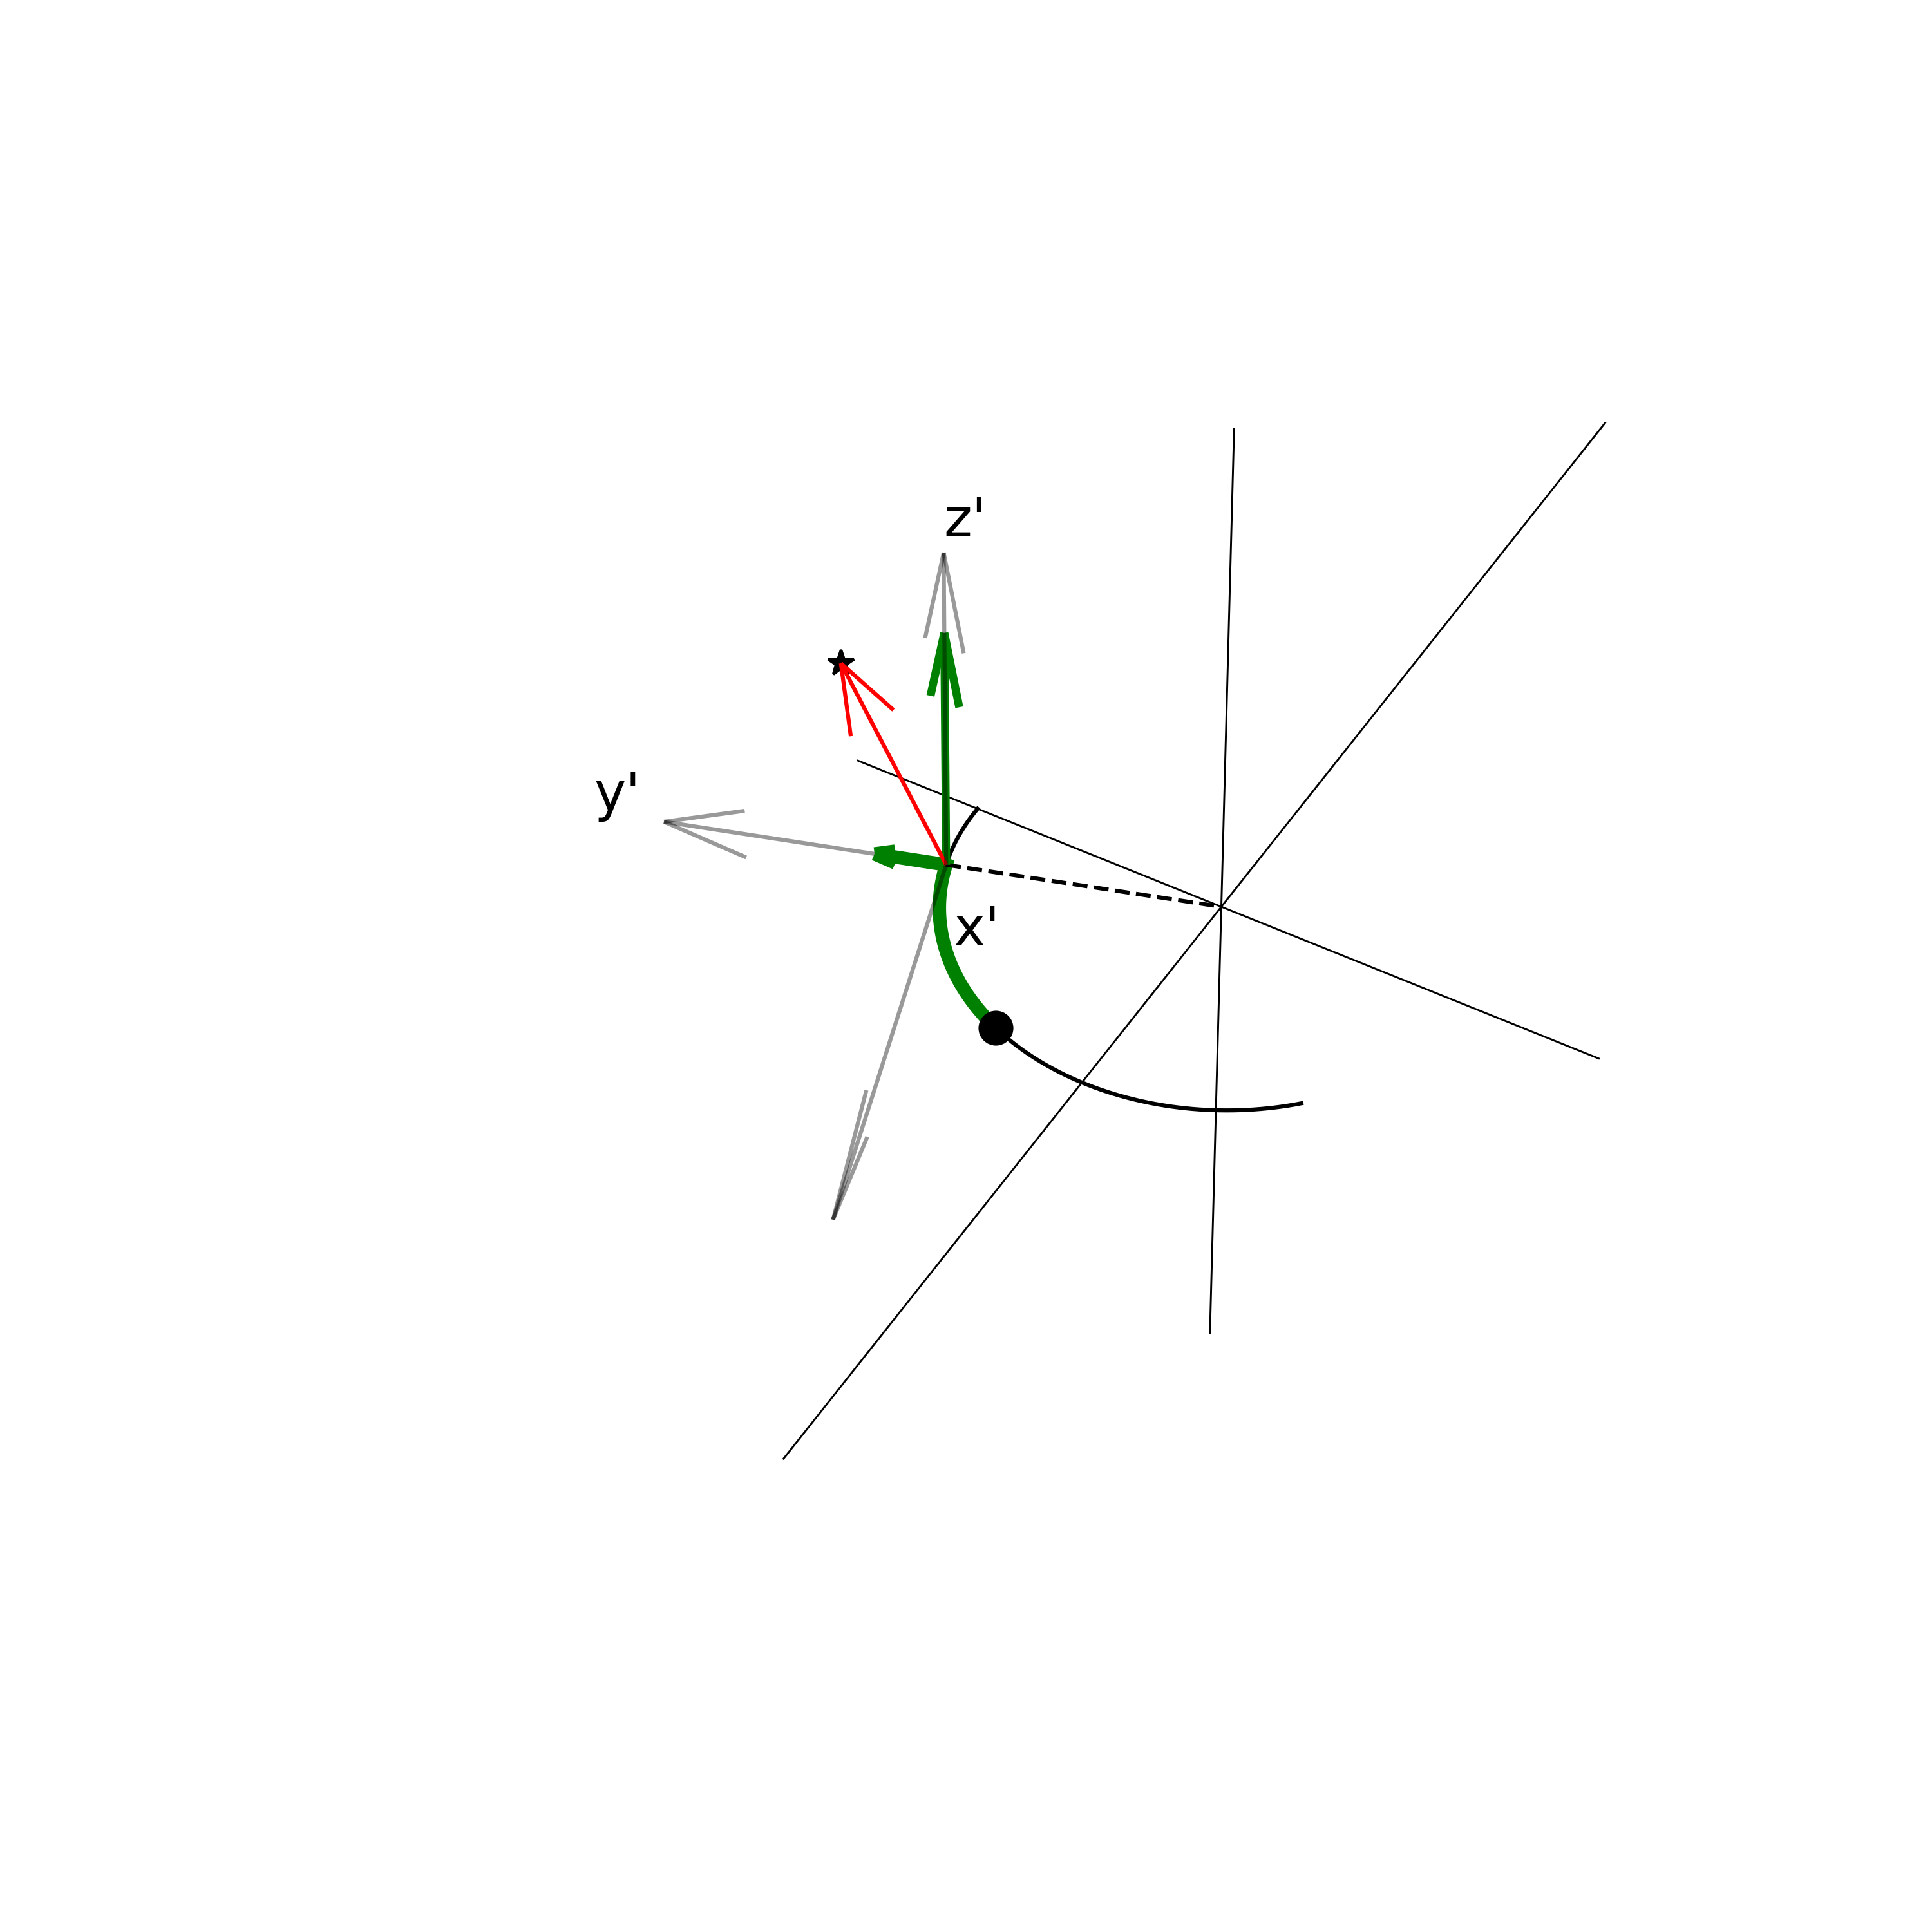
\includegraphics[width=\linewidth]{along_orbit_coordinate_system-approved.png}
      \caption{Tail coordinates. \textbf{I want to update this}. }
      \label{fig:TailCoordinates}
    \end{figure}
  
    \begin{figure*}
      \centering
      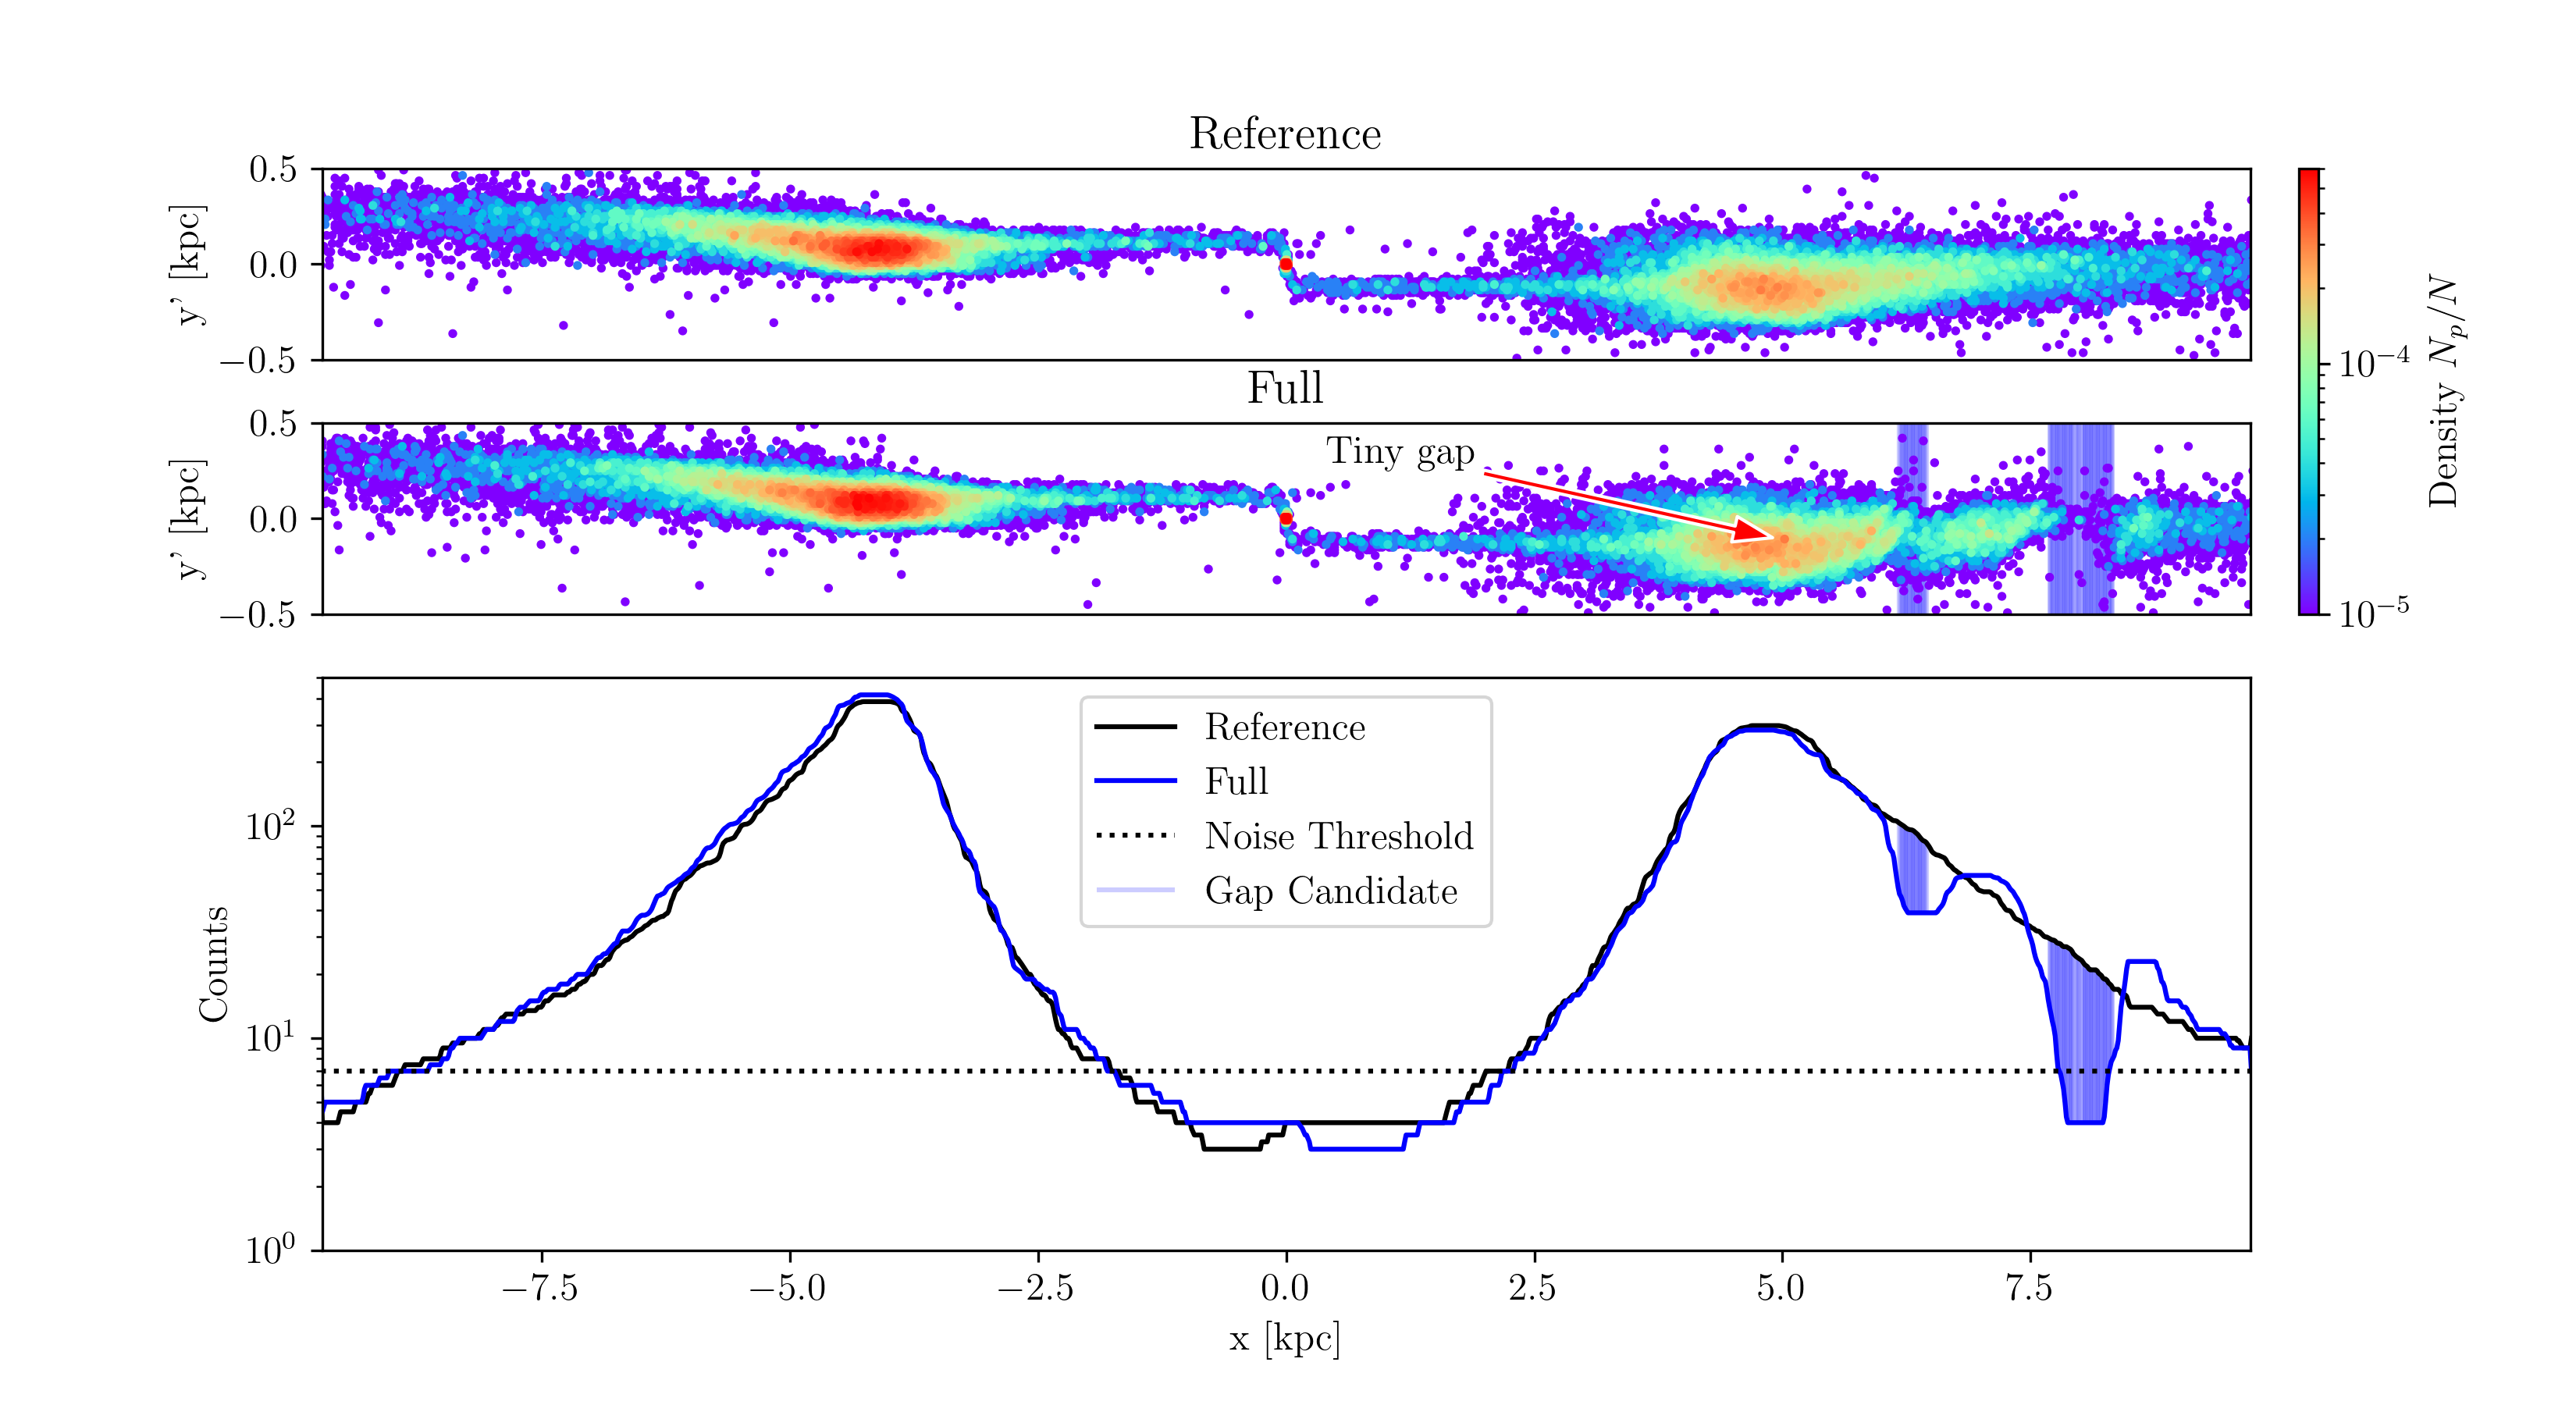
\includegraphics[width=\linewidth, trim=20 0 15 0]{monte-carlo-009-pouliasis2017pii-GCNBody-2000-milisigma-5-noisefactor-20-boxcarindexlength-shifted-0.png}
      \caption{A comparison between the density maps and profiles of the \texttt{full} and \texttt{reference} simulations is presented. The locations where the full simulation is less dense than the vanilla simulation by 2-$\sigma$ is highlighted by blue vertical bars. Bins below the noise threshold are not considered when measuring the differences between the two 1D profiles. The 1D profiles have been smoothed with a median box-car filter.}
      \label{fig:profiles}
      \end{figure*}

    To construct the 1D density profiles, we bin the data using the $\sqrt{N}$ rule, where $N$ is the number of data points ($N_p = 10^5$). After binning the 1D profiles, we apply a boxcar smoothing technique. The density profiles are scanned. This raw profile density curve is then smoothed with the median box-car filter. At each bin, a selected number of adjacent data points from both sides are placed in a list. The bin is then replaced with the median. We choose to use 10 adjacent points per side, which corresponding to a smoothing length of approximately 1~kpc. This procedure reduces high-frequency noise and smooths the profiles. For instance, notice the absence of a high mass peak indicating for the center of mass in the bottom panel of Fig.~\ref{fig:profiles}.

    With the smoothed 1D density profiles in hand, we search for regions where the \texttt{full} simulations are significantly underdense compared to \texttt{reference} simulations, surpassing stochastic fluctuations. To accomplish this, we first impose a signal-to-noise ratio threshold, $\mathcal{SNR}$. The signal is defined as the log of the counts per bin from the \texttt{vanilla} 1D density profile, and errors are propagated assuming a Poisson distribution. We then compute a threshold for the number of counts in the \texttt{vanilla} simulation, $N_v$, using the transcendental equation:
    \begin{equation}
        \mathcal{SNR} = \ln(10) \log_{10}\left(N_v\right) \sqrt{N_v}.
      \end{equation} \label{eq:density_threshold}
    By setting $\mathcal{SNR} = 5$, we solve for $N$ using \texttt{scipy.optimize.fsolve}, finding that $N$ must be greater than 7. After discarding insignificant bins (i.e., those with counts below the threshold), we compute the log ratio of the counts between the \texttt{vanilla} and full simulations:
    \begin{equation}
        \mathcal{R}_i = \log_{10}\left(\frac{N_{f,i}}{N_{v,i}}\right),
      \end{equation}
    where $\mathcal{R}_i$ is the log ratio, $N_{f,i}$ are the counts from the full simulation, and $N_{v,i}$ are the counts from the \texttt{vanilla} simulation for each bin $i$. We then analyze the distribution of $\mathcal{R}_i$. If the differences between the density profiles are primarily due to stochastic processes of similar magnitude, this distribution should resemble a Gaussian as expected from the central limit theorem. Thus, we flag all regions where the density is underdense by more than two standard deviations, which should highlight regions whose underdensity is unlikely to be the result of the sum of stochastic processess but rather the passage of another globular cluster. 

    This method, however, has its limitations, especially when detecting smaller gaps. As outlined by \citet{2015MNRAS.450.1136E}, a small gap is not indicative of a weak impact, but a recent one. This is because gap growth is a dispersion phenomenon. Additionally, since our streams have finite width, some gaps are oblique with respect to the stream axis. In such cases, marginalizing over $y'$ erases the gap's signal, making it impossible to detect in a 1D profile. This limitation is particularly evident in gaps caused by NGC~2808, as discussed in the results. Therefore, this quantitative analysis serves as an \textit{aid} to visual inspection rather than a complete substitute for it. This method helps particularly with large subtle gaps that the eye does not notice in the 2D maps. These profiles are included in the Appenix~\ref{sec:gallery_of_gaps}.


    \section{Perturber Identification} \label{sec:Perturber_Identification}

      A key question we seek to answer is: from the gaps present at the end of the simulation, who caused them? To address this, we examine the evolution of stream density over time. Instead of using the x'-coordinate, we introduce $\tau$, which represents time rather than distance. Specifically, $\tau$ indicates how long it will take for a cluster to reach, or how long ago it passed, a given point on its orbit. This is advantageous because the growth of the stream is approximately linear in $\tau$ whereas in physical space, streams on eccentric orbits expand and contract depending on the orbital phase.


      \citet{2016MNRAS.457.3817S} extended the analysis of \citet{2015MNRAS.450.1136E}, demonstrating that action-angle variables provide a useful coordinate system for analyzing stream evolution, as actions are conserved and the angles associated with the stream's growth evolve linearly over time. Although we became aware of this work only after completing our analysis, we note that $\tau$ is a suitable approximation and behaves similarly to the angle variable corresponding to the azimuthal action: $\tau \approx \theta_{\phi,i} - \theta_{\phi,\text{GC}}$.

      The core of our analysis is presented in Fig.~\ref{fig:force-on-orbit}. The bottom panel shows the evolution of the stream density over time. To avoid extreme low-density regions at the stream's edges, we applied the same density threshold as from eq.~\ref{eq:density_threshold} to focus on the more significant areas of the stream. Next, we modeled Palomar~5's orbit as a proxy for its stream and sampled points along the orbit to measure the gravitational force exerted by other globular clusters. This force data is displayed in the top panel of Fig.~\ref{fig:force-on-orbit}, showing how the total gravitational acceleration on Palomar 5's stream evolves over its length throughout the simulation.

      \begin{figure*}
        \centering
        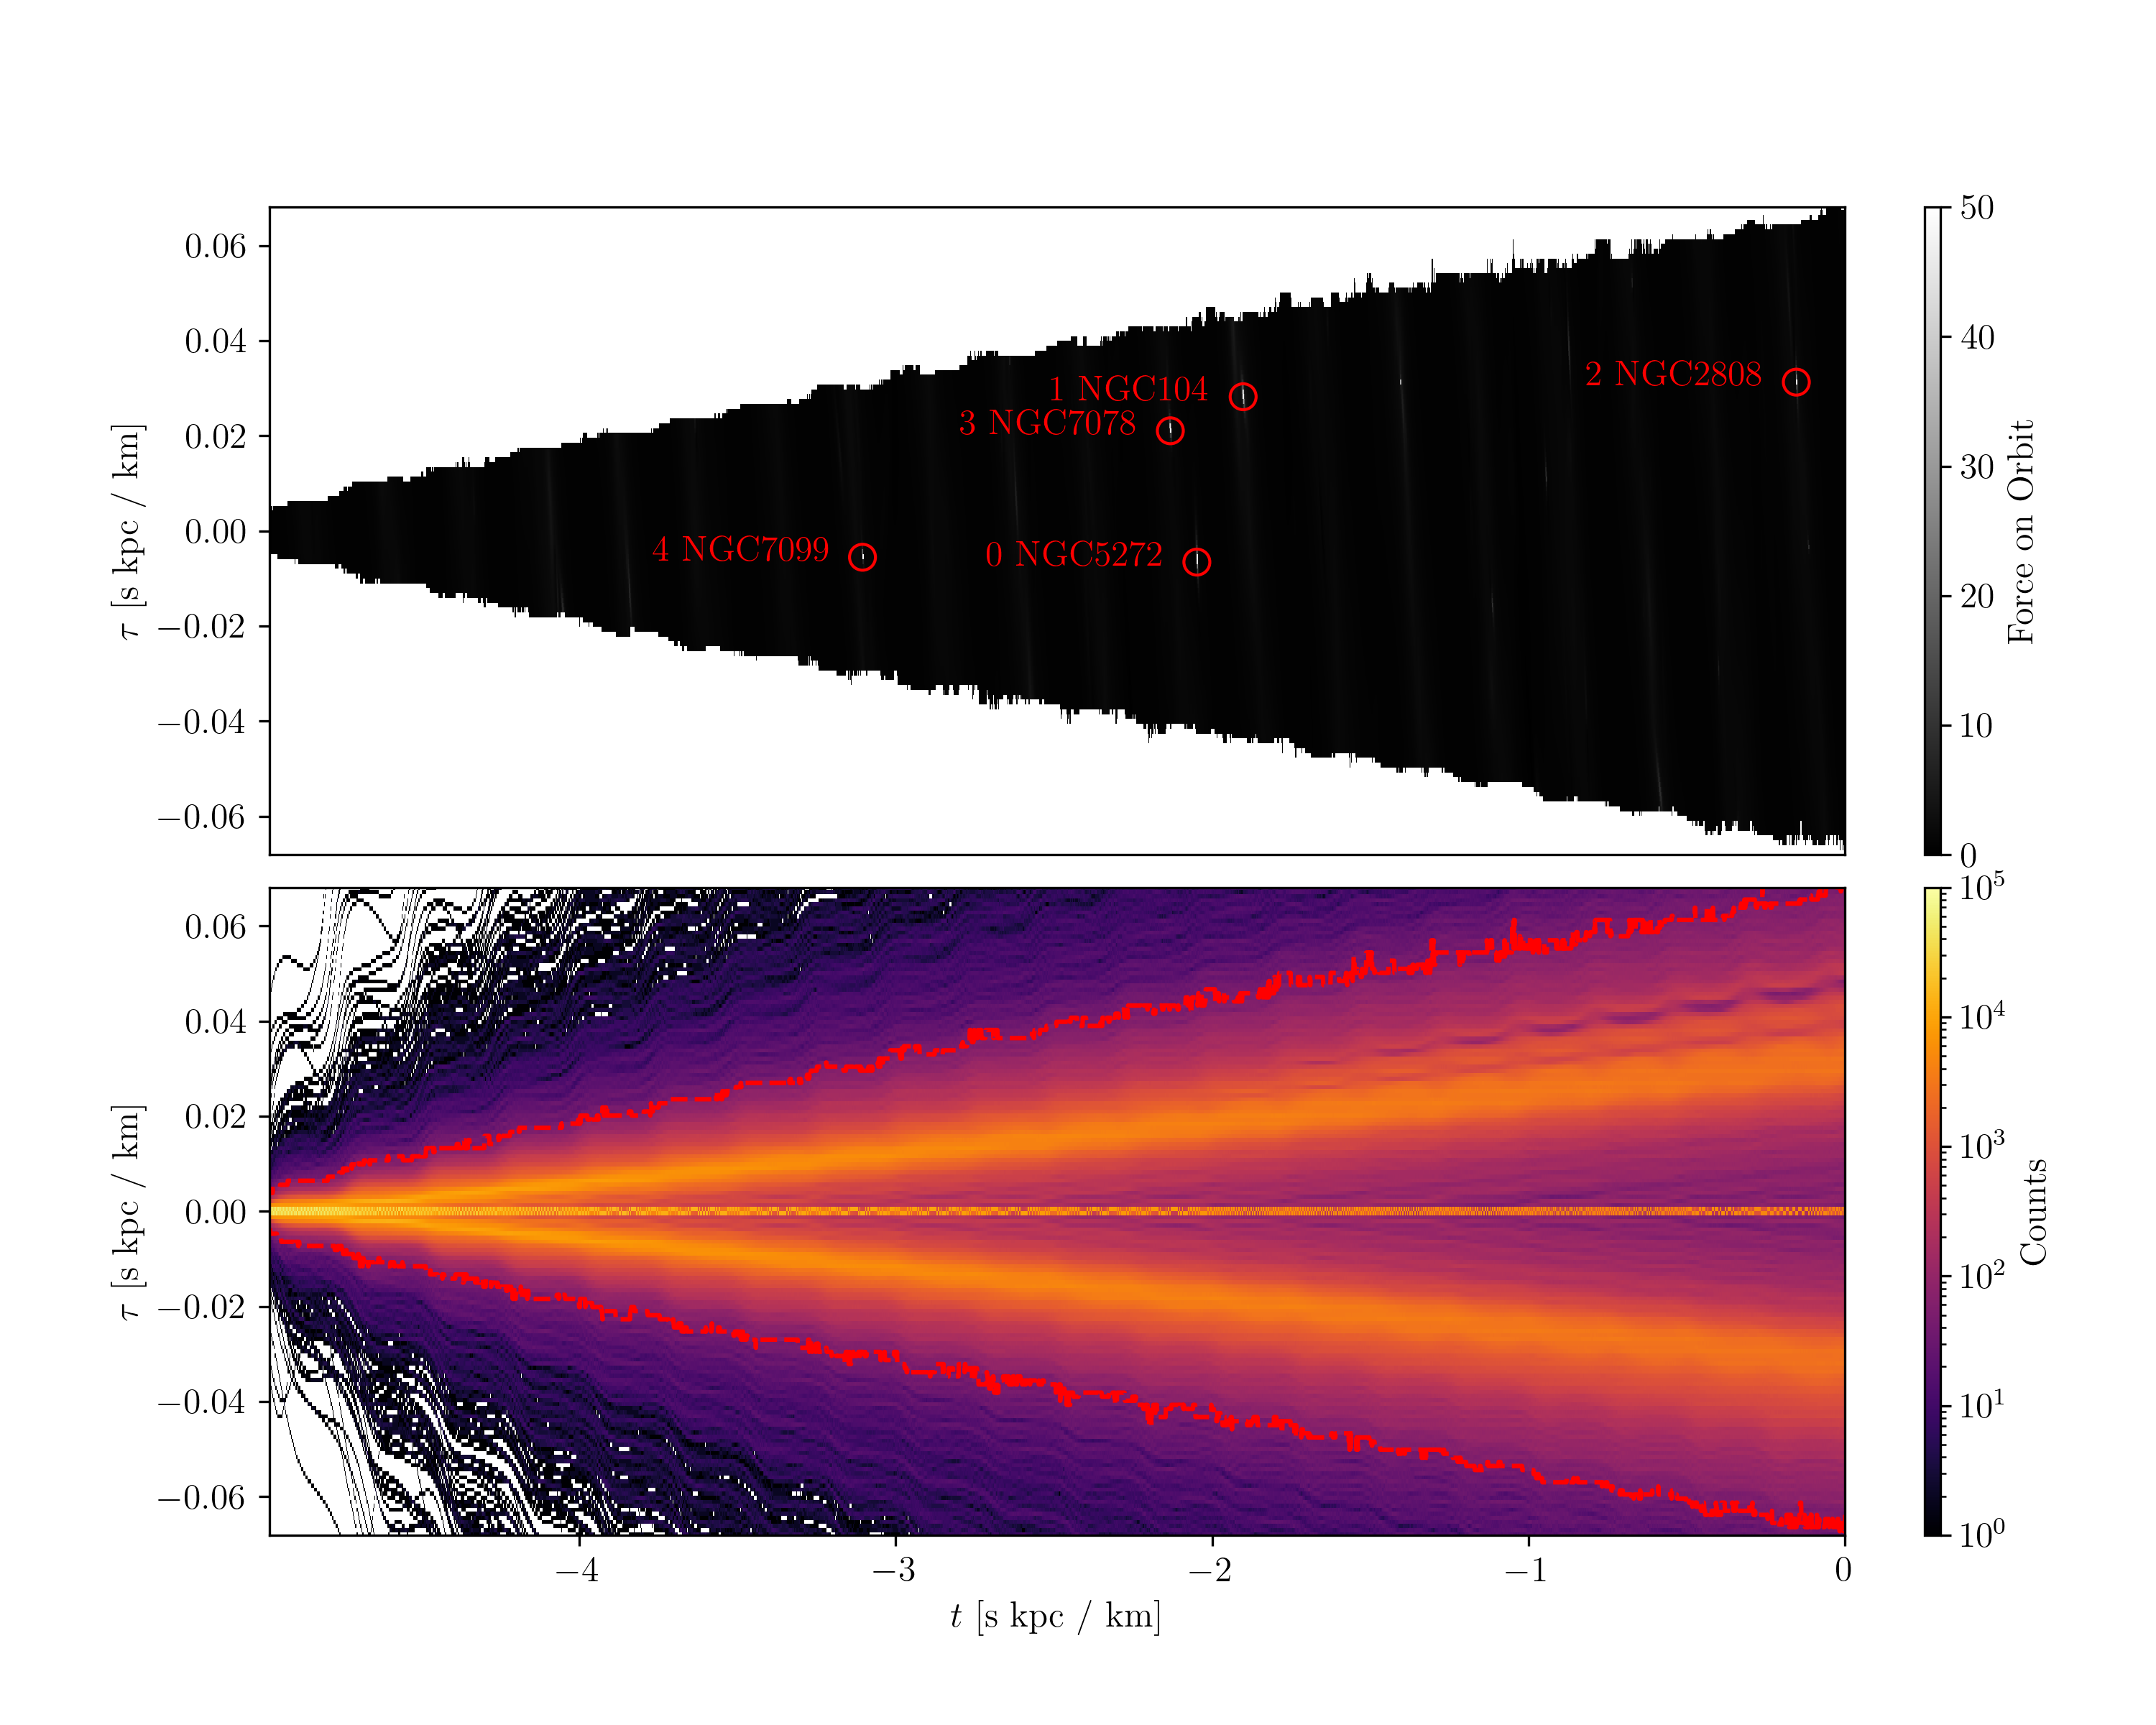
\includegraphics[width=\linewidth]{force_on_orbit-monte-carlo-009.png}
        \caption{This figure demonstrates how we determined which globular clusters were responsible for the gaps. The y-axis is $\tau$, which is a coordinate in units of time that indicates how far ahead or behind it is from a globular cluster. The x-axis is the simulation time, $t$, where 0~s km~kpc$^{-1}$ indicates present time.  The bottom plot showcases the evolution of the stream density in simulation time. The density was used to determine a sutible length of the stream at a given function. This length was then used to extract a piece of Palomar 5's orbit. This orbital segment is used to approximate the stream. Then, the gravitational force from all other clusers was computed on the orbit. This is shown in the top plot, where the gravitational force is in measured in acceleration and is given in integration units: km$^2$~kpc$^{-1}$~s$^{-2}$. Moments of high acceleration indicate the passage of another cluster. The top 5 strongest passages are labeled with red circles as well as the name of the clusters. The example shown in this plot is the same simulation as Fig.~\ref{fig:stream_on_sky}.}
        \label{fig:force-on-orbit}
      \end{figure*}  


      We then used \texttt{scipy}'s \texttt{ndimage} \citep{2020NatMe..17..261V} package to identify the top five local maxima in the data space of gravitational acceleration $\vec{g}$ as a function of time $t$ and the stream coordinate $\tau$. This is done by first smoothing the image by taking a 5 point moving average kernel. Secondly, we use maximum filter to locate coordinates in the $t,\tau$ data plane who are local maxima to at least 10-adjacent data points. These locations are then ordered and the top five strongest interactions are saved. Once these local maxima were identified, we iterated over the contributions of individual globular clusters to determine which cluster contributed the most to each peak in $\vec{g}$. Each significant peak was labeled with the corresponding globular cluster.


      Afterward, we cross-referenced these peaks with the locations of the gaps identified by studying the density maps and profiles from Fig.~\ref{fig:profiles}. For large gaps resulting from strong interactions, we observed that after an impact, a low-density wake is left behind in the ($t,\tau$) plane, which can be seen corresponding to the impacts of NGC~104 and NGC~7808 in the bottom panel of Fig.~\ref{fig:force-on-orbit}.



      Fig.~\ref{fig:force-on-orbit} contains some interesting information. Notice the periodic ribbions of force in the $(t,\tau)$ plane. This is due to pericenter passages where Palomar~5 is getting closer to the center of mass of the globular cluster system. Additionally, for the impacts of NGC~104 and NG~C7078, wakes can be observed in the density map. Another important aspect, is that the strongest peak in gravitational force does not necessarily create a gap. Notice how NGC~5272, which was labeled with 0 to indicate that it has the greatest local maxima does not have a gap. The reason for this is manifold, for instance, the force needs to be modulated with the time since the change in momentum is the determining factor and not the peak magnitude of the force.  Additionally, there is an offset of about 200~pc between the stream at the orbit, as seen when viewing the stream in tail coordinates, so peaks upon the orbit are good proxy's for the stream but are not definitive. We found that the top five greatest impacts accounted for all gaps, except for Sampling~014 as shown in Fig.~\ref{fig:gallery3}, whose gap from NGC~6584 corresponded to the 7th peak. 

      The results of this analysis were compiled into a table. If a gap was attributed to a particular globular cluster, it was labeled as \texttt{TRUE}; otherwise, it was marked as \texttt{FALSE}. For a handful of simulations, to double check that the verdict made correctly when passing from suspect to culprit, we re-compute the simulations yet individually adding one globular cluster at a time. As a result, we are able to confirm that singular gaps arrise from the suspected clusters, an example of which is shown in Fig.~\ref{fig:decomposition}. 



    \section{Reconstruction of the impact geometry} \label{sec:reconstruction}

      With the perturbers identified, we perform statistics in the pursuit of understanding what conditions are necessary for a globular cluster and a stream to have in order for a gap to form. We turn to impact theory, which in its simplest form is presented in works such as \citet{2008gady.book.....B}.Consider two particles: one stationary and the other moving past it. The distance between the two particles at their closest approach is known as the impact parameter. To simplify the analysis, the \textit{impulse approximation} is employed, which assumes that the velocity of the perturber remains unchanged during the interaction. This assumption simplifies the computation.

      To understand how the impacted particle is perturbed, one needs to compute its change in momentum, which is determined by integrating the force acting on the particle over the duration of the interaction. A useful approximation for this change in momentum is the force at the closest approach multiplied by an estimate of the interaction time:
      \begin{equation} 
        \Delta p \approx \text{Force} \times \text{interaction time} = \frac{GMm}{b^2} \times 2\frac{b}{v} = 2\frac{GM}{bv}, 
        \end{equation} 
      where $M$ is the mass of the perturber, $m$ is the mass of the particle, $b$ is the impact parameter, $v$ is the relative velocity of the perturber with respect to the particle, and $G$ is the gravitational constant.

      From this analysis, we can conclude that a more massive perturber, passing closer to the particle, and moving more slowly, will have a greater impact. It's important to note that the momentum change is inversely proportional to the velocity of the perturber, which contrasts with the intuition from elastic collisions, such as those between billiard balls, where higher velocities result in greater impacts.

      \citet{2015MNRAS.450.1136E} extended this impact theory from one point mass impacting another point mass, to studying how an extended body impacts as stream. This quantifies the change in momentum of a given particle as a function of its distance from the point of greatest impact. In their analysis, the perturber was modeled as a Plummer sphere, like in our simulations. Since the stream is not zero-dimensional and has length, both the parallel and perpendicular components of the pertuber's velocity must be considered. Consequently, five parameters determine the change in velocity of a given stream particle: $M$, $r_p$, $b$, $W_\parallel$, and $W_\perp$. We set out is to constrain these parameters during the impact in our simulations and compare them to close approaches that do not generate gaps, in order to establish the criteria necessary for gap formation.

      To achieve this, we begin by identifying the approximate moments of impact from the most significant clusters, as determined in the previous analysis in Sec.~\ref{sec:Perturber_Identification}. Then, we refine these estimates in oredr to to pinpoint both the exact location of the impact along the stream and the precise moment it occurred. To do so, we fit a third-order parametric polynomial to the stream, using the saved snapshots from our simulations:
      \begin{equation}
        \vec{s}(\tau) = 
        \left\{
          \begin{aligned}
            x(\tau) &= a_0 + a_1 \tau + a_2 \tau^2 + a_3 \tau^3 \\ 
            y(\tau) &= b_0 + b_1 \tau + b_2 \tau^2 + b_3 \tau^3 \\
            z(\tau) &= c_0 + c_1 \tau + c_2 \tau^2 + c_3 \tau^3
          \end{aligned}
        \right.
        \end{equation}  
      where $x$, $y$, and $z$ represent the parametric line describing the stream in galactocentric coordinates, $\tau$ is the stream coordinate in time as described in the Appendix~\ref{sec:Perturber_Identification}, and is used as the independent variable to parameterize the position along the stream. The coefficients $a_i$, $b_i$, and $c_i$ are the polynomial coefficients. We found that a second-order polynomial was insufficient to capture the curvature along the full length of the stream, with divergence at the ends of the tails. A third-order polynomial was sufficient and desirable, as it is the lowest order that adequately captures the path of the stream over the entire length under consideration.

      In this analysis, only one side of the stream is considered. For instance, if the impact candidate was in the leading tail, only the star particles with $\tau > 0$ are used to constrain the stream track. The polynomial coefficients were determined using the through a minimization method using Nelder-Mead algorithm from \texttt{scipy}'s optimization package.

      Since the simulation snapshots were saved at a temporal resolution of 1 Myr--—rather than at the integration timestep, which would have generated an excessive amount of data—--we interpolate between snapshots to more precisely estimate the impact geometry. This is achieved by fitting the stream at five timesteps surrounding the approximate impact time, a period of 5 Myr, which sufficiently covers the interaction time. The interaction time can be estimated as $t \approx \frac{100~\text{pc}}{300~\frac{\text{km}}{\text{s}}} \approx 0.3~\text{Myr}$.

      As a result, each polynomial coefficient can now be expressed as a function of time. Consequently, we can parameterize the stream as a function of both simulation time and position along the stream:
      \begin{equation}
        \vec{s}(t,\tau) = 
        \left\{
        \begin{aligned}
          x(t,\tau) &= a_0(t) + a_1(t)\tau + a_2(t) \tau^2 + a_3(t)\tau^3 \\ 
          y(t,\tau) &= b_0(t) + b_1(t)\tau + b_2(t) \tau^2 + b_3(t)\tau^3 \\
          z(t,\tau) &= c_0(t) + c_1(t)\tau + c_2(t) \tau^2 + c_3(t)\tau^3.
          \end{aligned}
        \right.
      \end{equation}
      The values of the coefficients as a function of time are obtained through linear interpolation, ensuring that the coefficients at the snapshot times match the values constrained by the simulation data.

      Next, we fit the trajectory of the perturber with a second-order polynomial. With equations for both the stream and the perturber as functions of time, we identify the time and location of impact by minimizing a cost function, defined as the distance between the stream and the perturber:
      \begin{equation} 
        b(t, \tau) = \left\lVert \vec{s}(t, \tau) - \vec{p}(t) \right\rVert, 
        \end{equation}
      where $\vec{s}(t, \tau)$ is the galactocentric position of a point on the stream, $\vec{p}(t)$ is the position of the perturber, and $b$ is the distance between the two. The minimum value of $b$, denoted as $\text{min}(b)$, represents the impact parameter. The minimization is carried out using \texttt{scipy}'s optimization package with the \textit{L-BFGS-B} method, which allows us to place bounds on $t$ and $\tau$, ensuring no extrapolation occurs.

      Once this minimization is performed, determining the relative velocity becomes straightforward. Since the minimization provides the impact parameter, time of impact, and corresponding value of $\tau$, we can compute the derivatives of the parametric equations at $t_{\text{min}}$ and $\tau_{\text{min}}$. The parallel and perpendicular components of the perturber's velocity relative to the stream are given by:
      \begin{equation}
        \begin{aligned}
          \delta \vec{v} &=\vec{v_p} - \vec{v_s} \\
          w_\parallel &= \left(\delta \vec{v}\right)\cdot \hat{v_s}\\  
          w_\perp &=  \sqrt{\Delta v ^2 - w_\parallel ^ 2}
          \end{aligned}
        \end{equation}
      where $\vec{v}_p$ and $\vec{v}_s$ are the velocities of the perturber and the stream, respectively. For each of the 50 simulations, this information was compute for the strongs 5 flybys of a perturber with the stream. Thus, we compute a sample of 250 impacts, and flag those that give way to gaps. 


      Visual inspection of the five key impact parameters ($M$, $r_p$, $b$, $W_\parallel$, and $W_\perp$) did not reveal a clear distinction between flybys that create gaps and those that do not. Due to the clutter, we omit this graph and instead present Fig.\ref{fig:impact_geometry_statistics}, which uses the total relative velocity rather than separating parallel and perpendicular components. We also exclude the characteristic radius, as it showed little correlation with the results, likely due to the narrow range of globular cluster radii (see Fig.\ref{fig:mass_size_plane}). This factor might be more significant for dark matter subhalos, where size variation is greater.
      
      
      \begin{figure*}
        \centering
        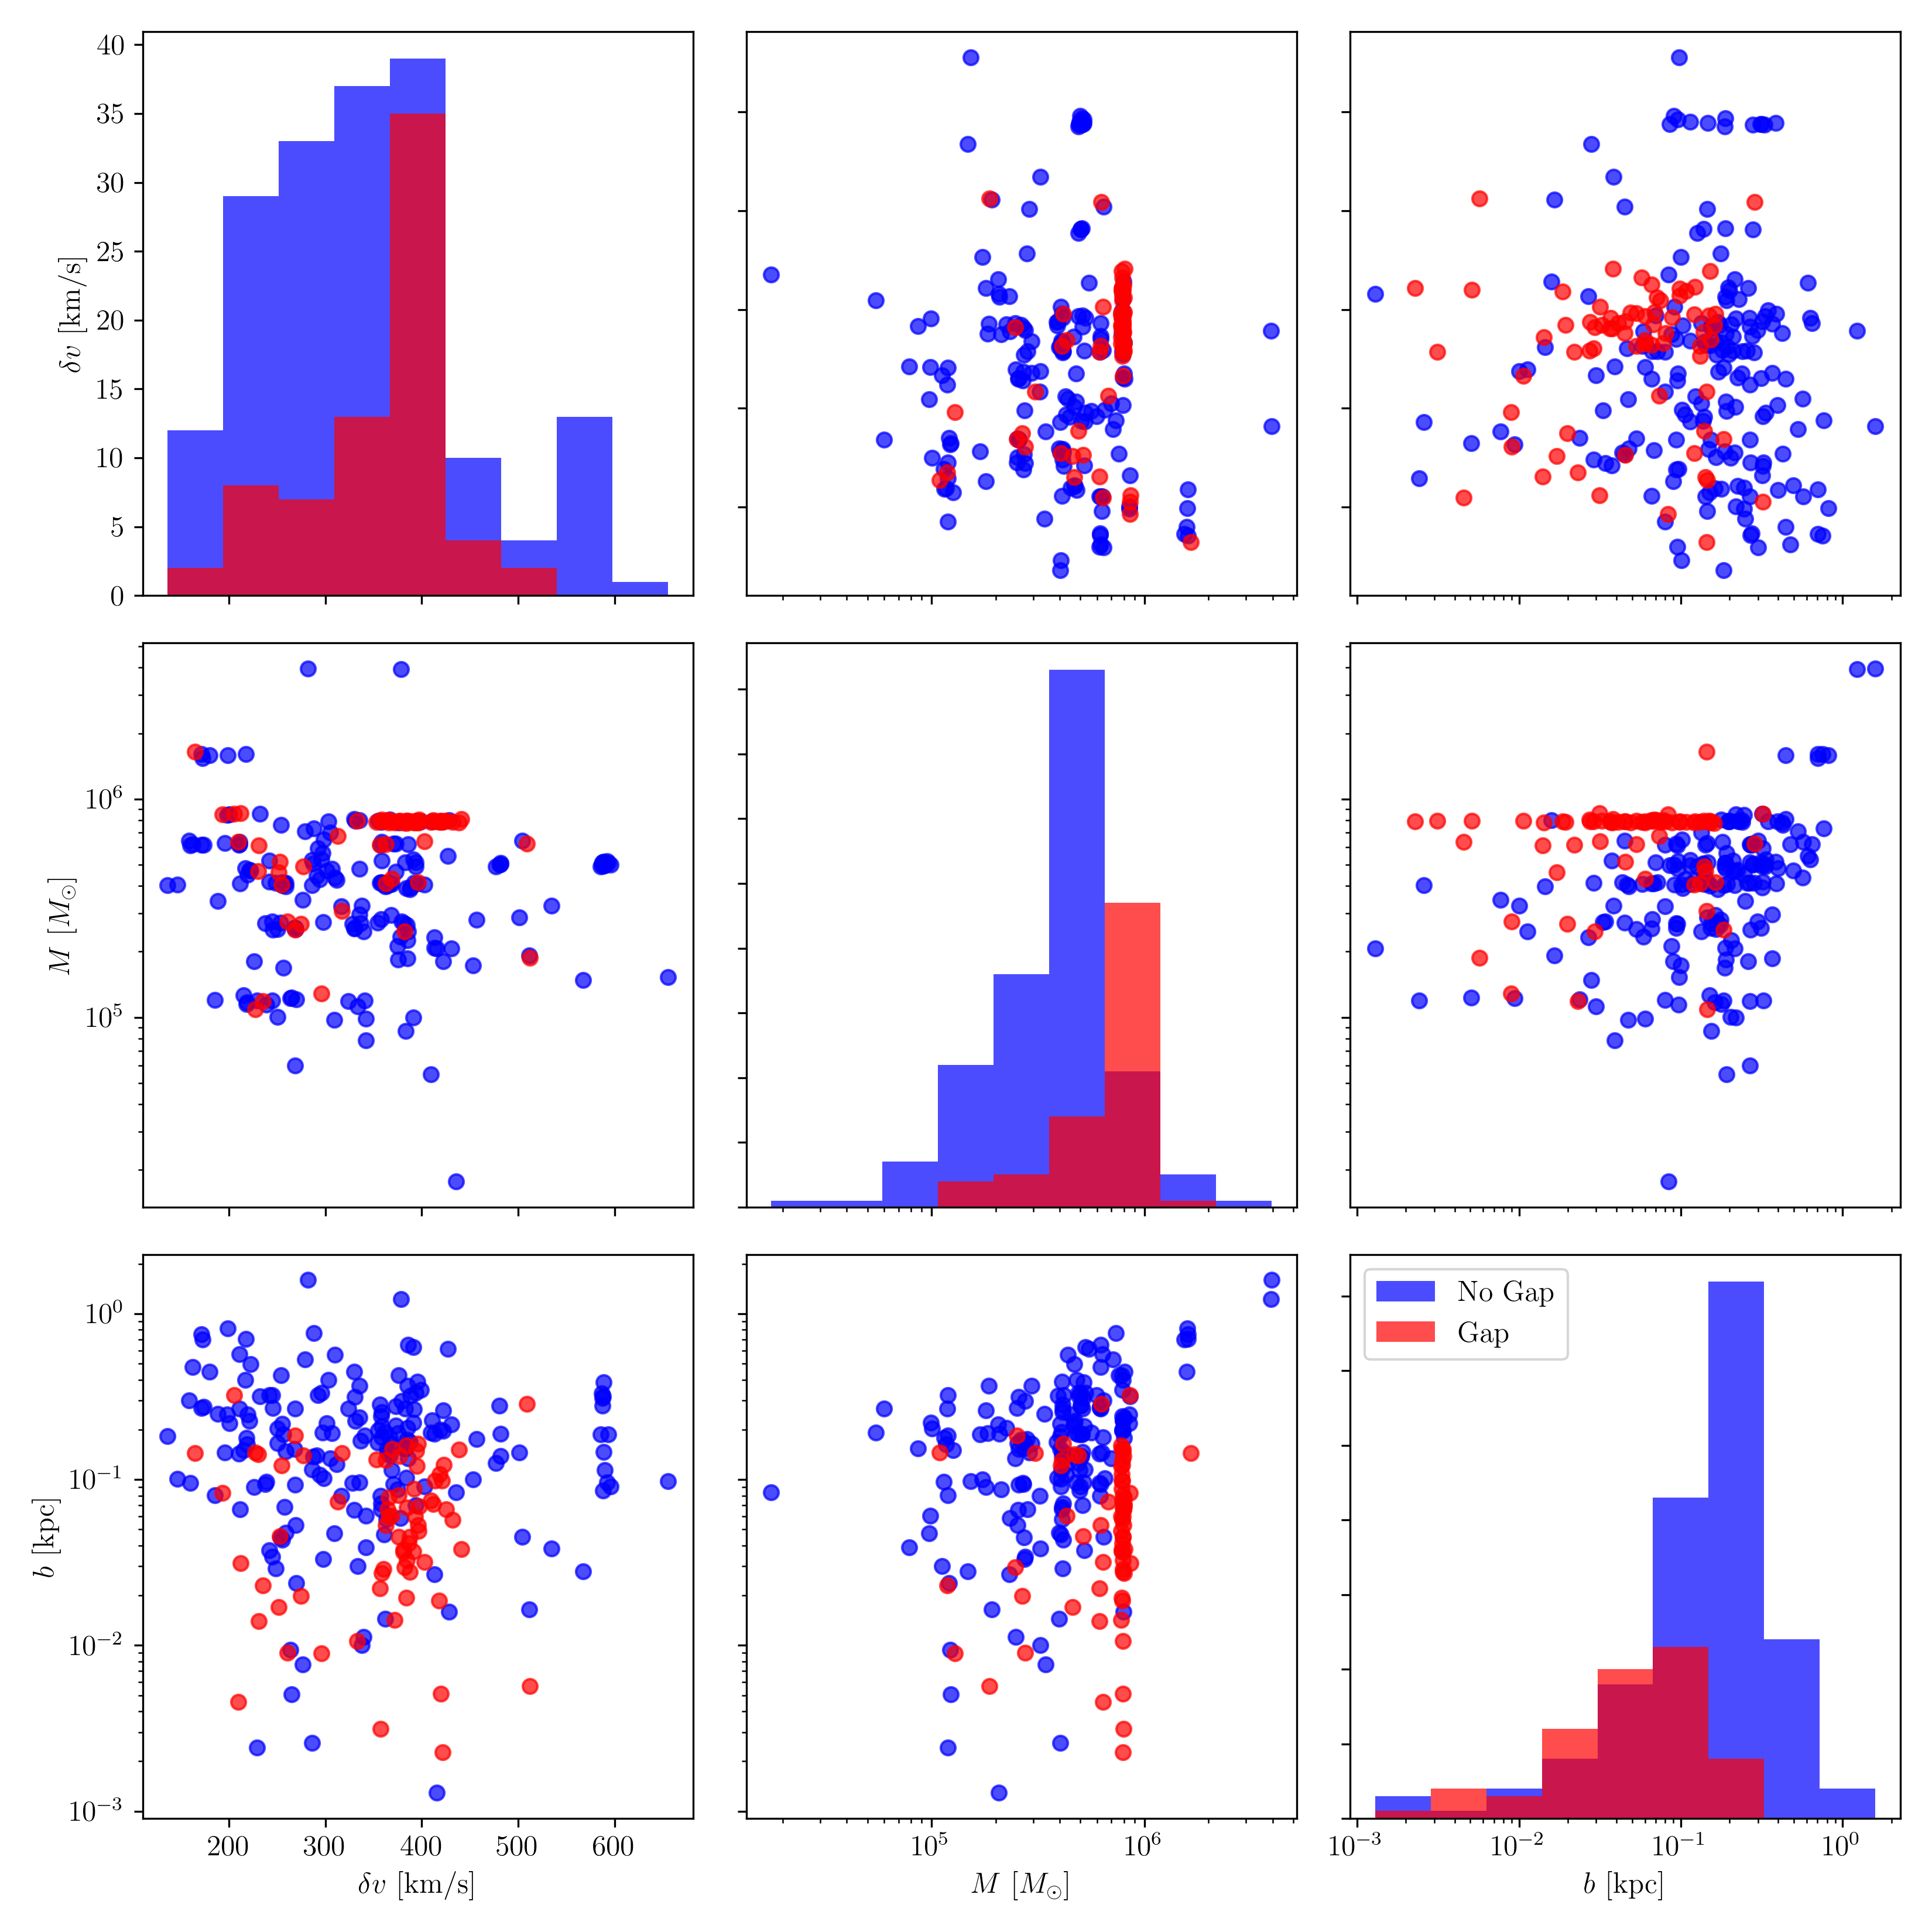
\includegraphics[width=\linewidth]{impact_geometry_statistics.png}
        \caption{The distribution and relationship between the basic impact variables from Eq.\ref{eq:change_in_momentum} and the close encounter that cause impacts, shown in red against those that do not, shown in blue. }
        \label{fig:impact_geometry_statistics}    
        \end{figure*}

      While Fig.\ref{fig:impact_geometry_statistics} demonstrates that mass, relative velocity, or impact parameter alone (from Eq.\ref{eqeq:change_in_momentum}) cannot predict gap formation, one interesting result emerges: no gaps are created from interactions with impact parameters greater than 200~pc. The stream widths are roughly 200~pc, with a radial thickness of about 100~pc. This finding is even more evident when examining the $b$-$M$ plane. A series of perturbers at roughly $\sim7 \times 10^5 M_\odot$ highlights NGC~2808's flybys, where all encounters with impact parameters under 200~pc result in gaps, while those beyond this distance do not.
        
        


  \section{Gallery of Gaps} \label{sec:gallery_of_gaps}

    \begin{figure*}
      \centering
      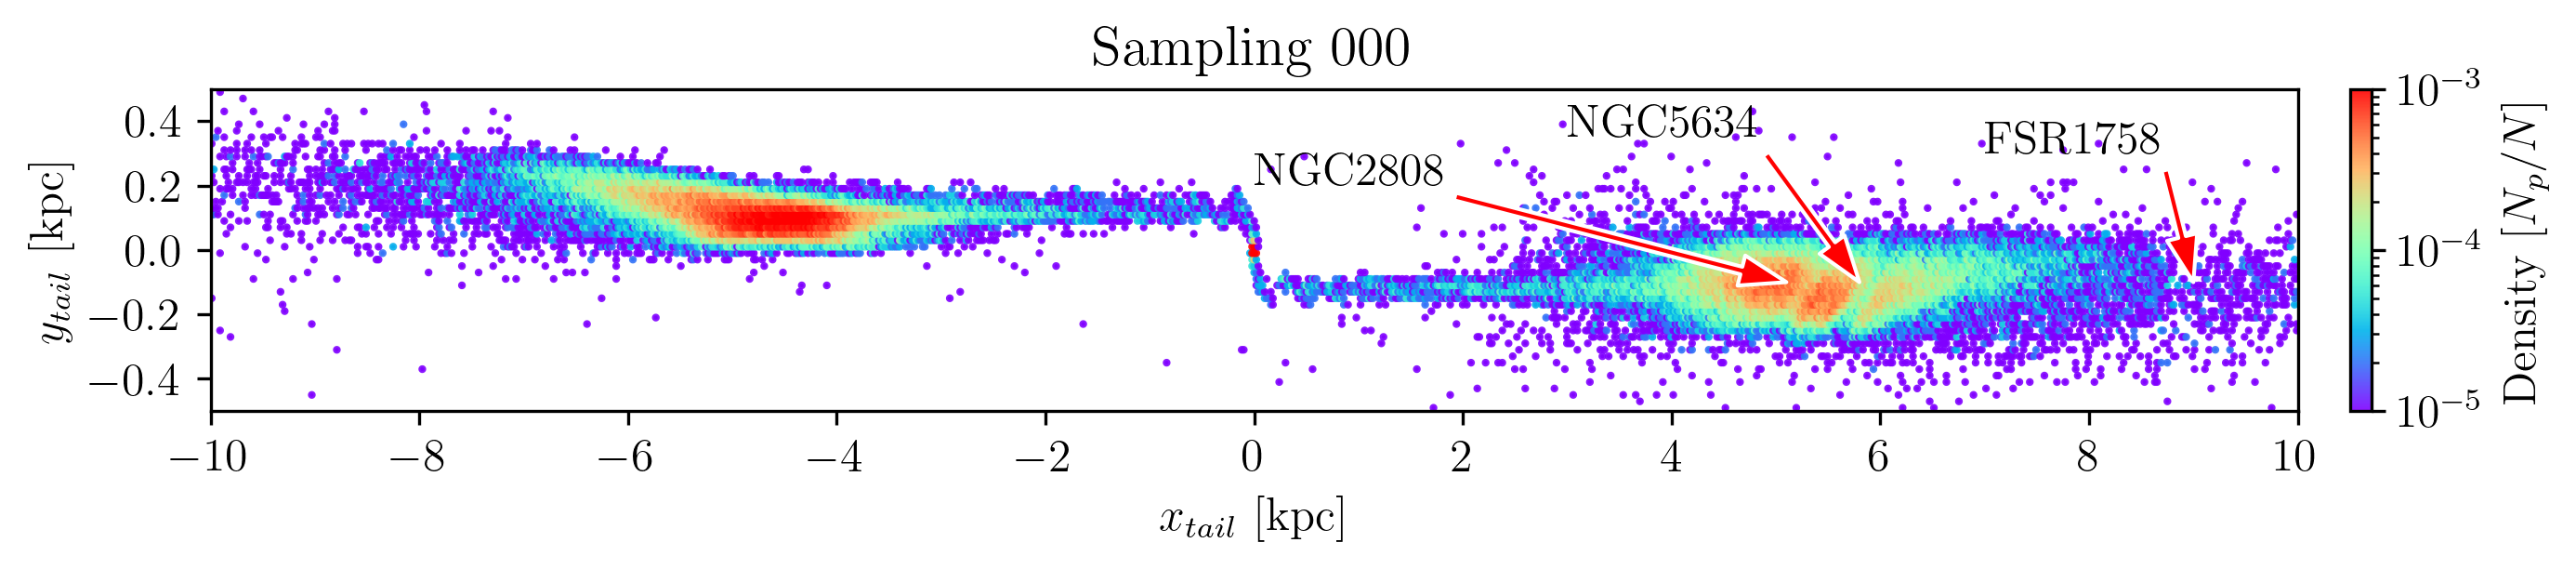
\includegraphics[width=\linewidth]{gallery_of_gaps_monte-carlo-000.png}
      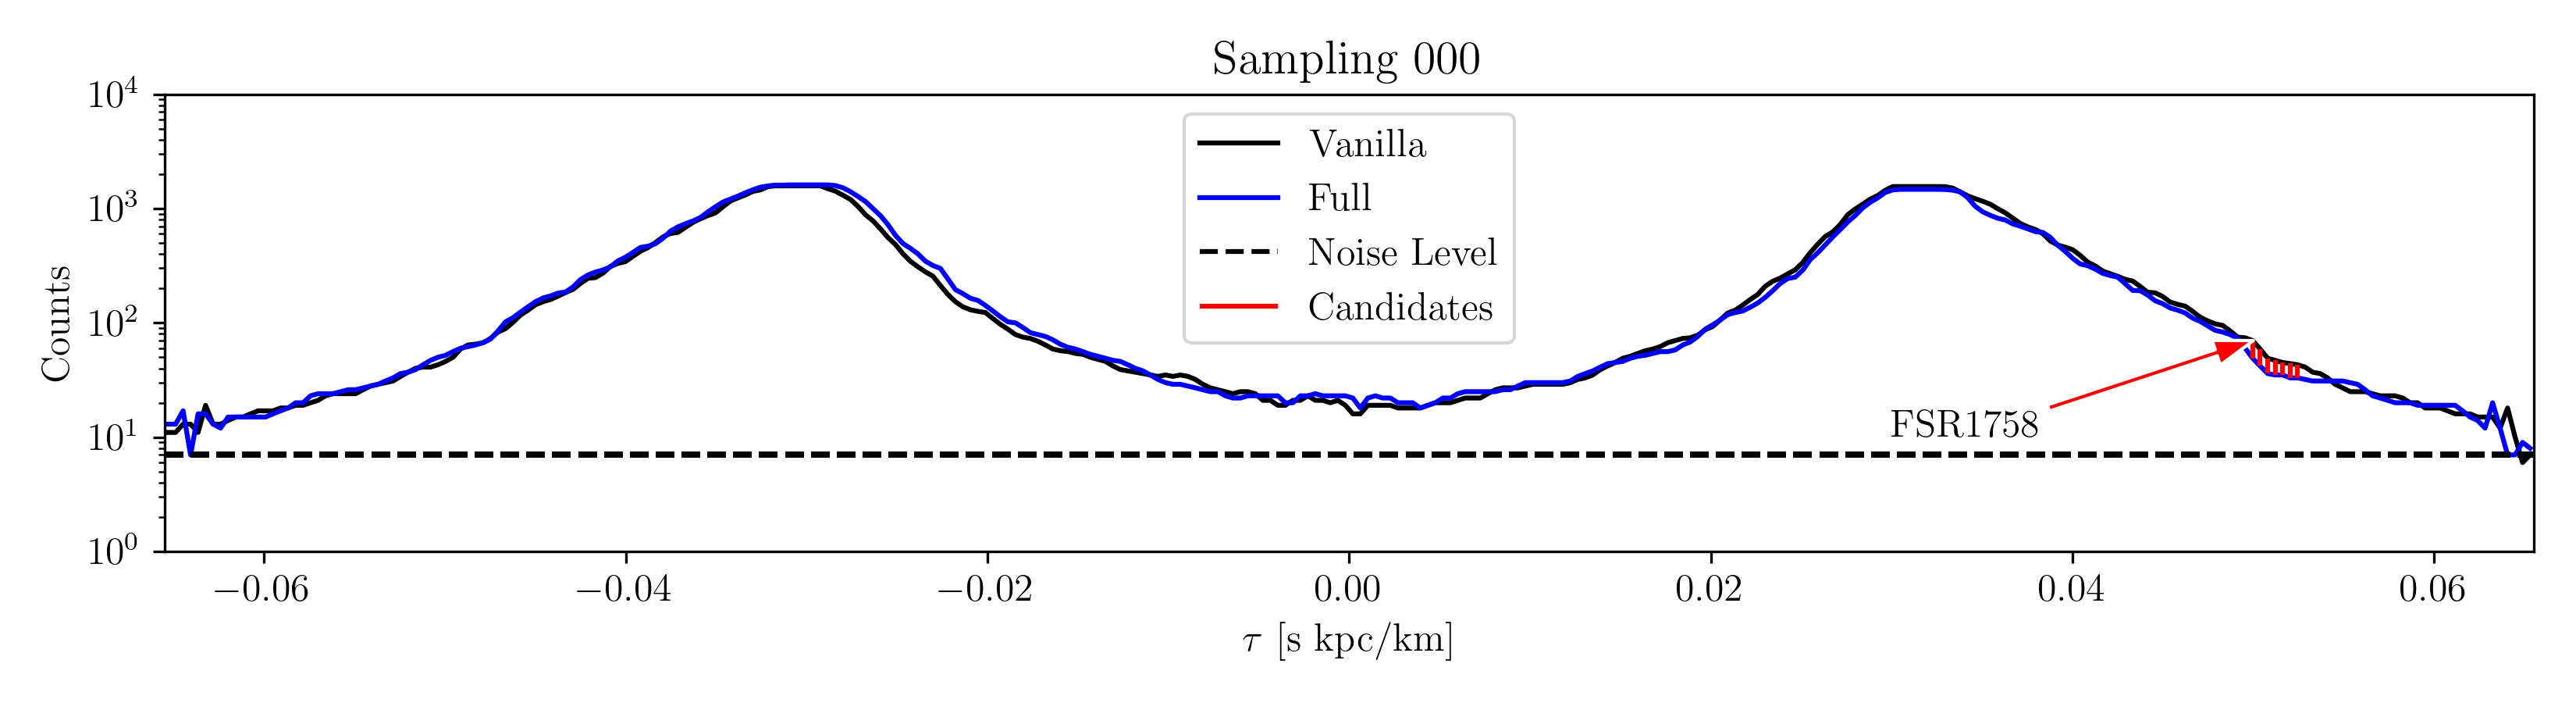
\includegraphics[width=\linewidth]{tau-profile-monte-carlo-000.png}
      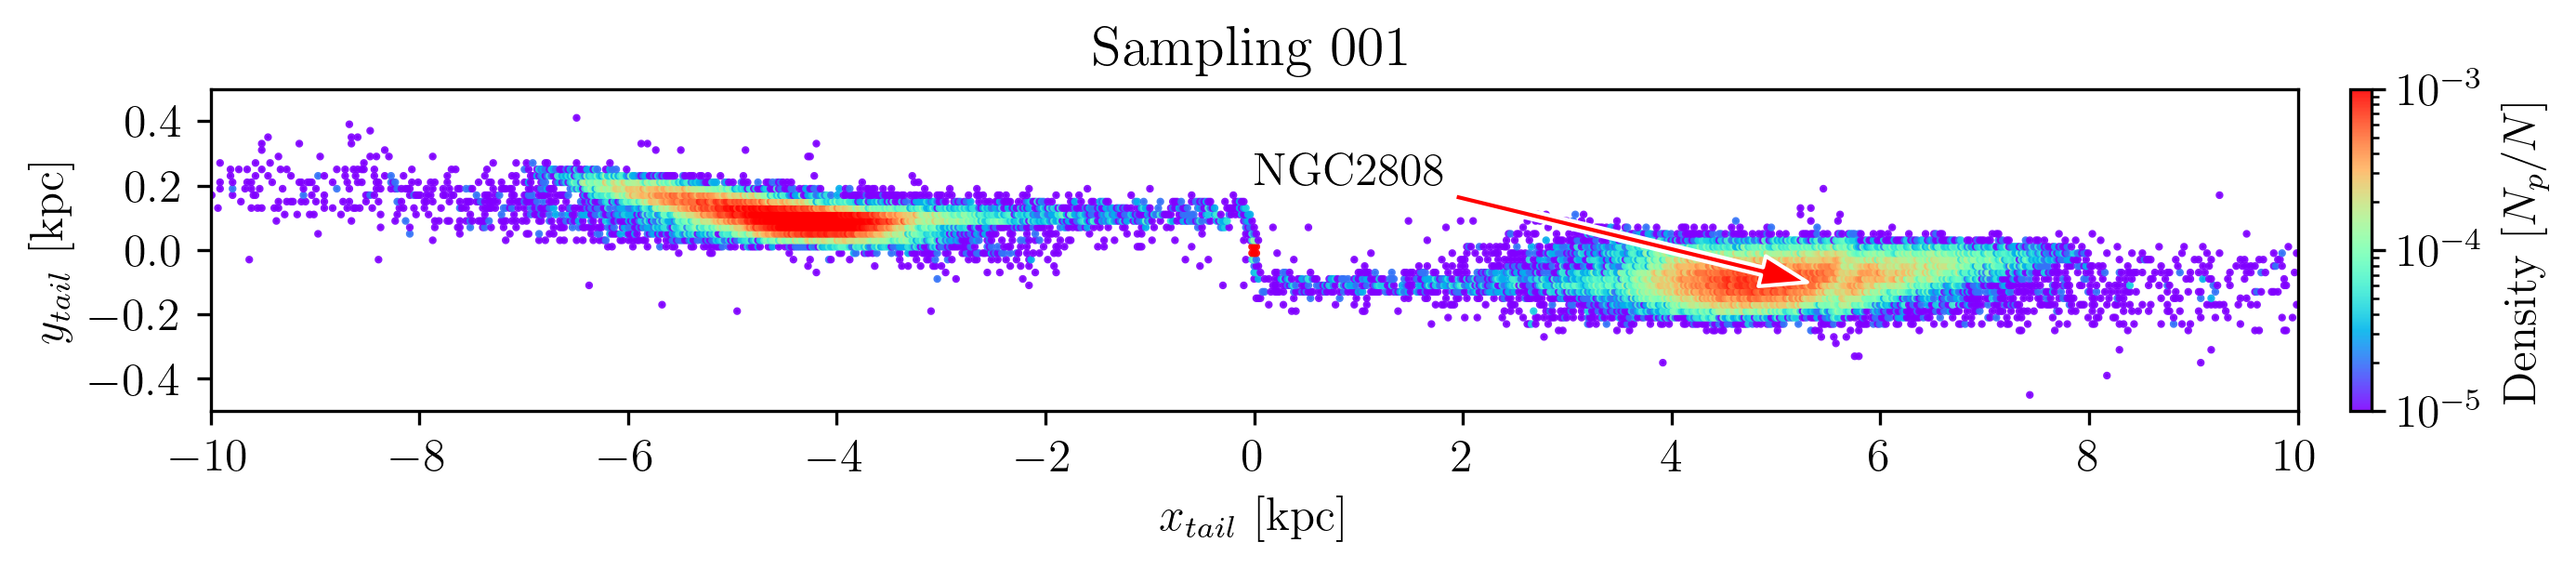
\includegraphics[width=\linewidth]{gallery_of_gaps_monte-carlo-001.png}
      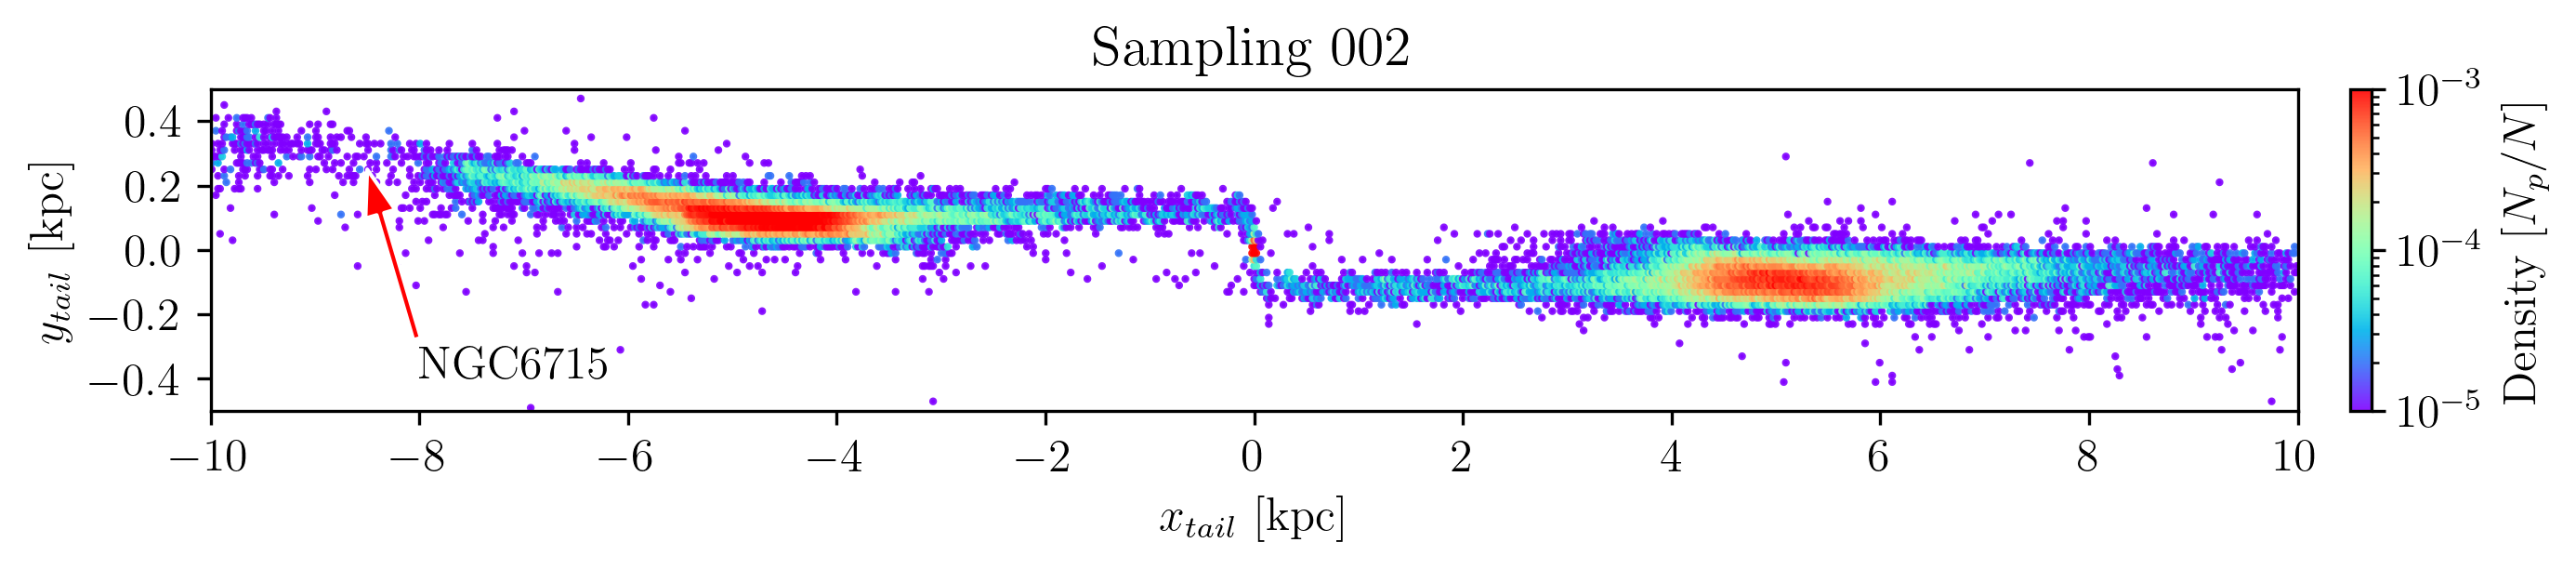
\includegraphics[width=\linewidth]{gallery_of_gaps_monte-carlo-002.png}
      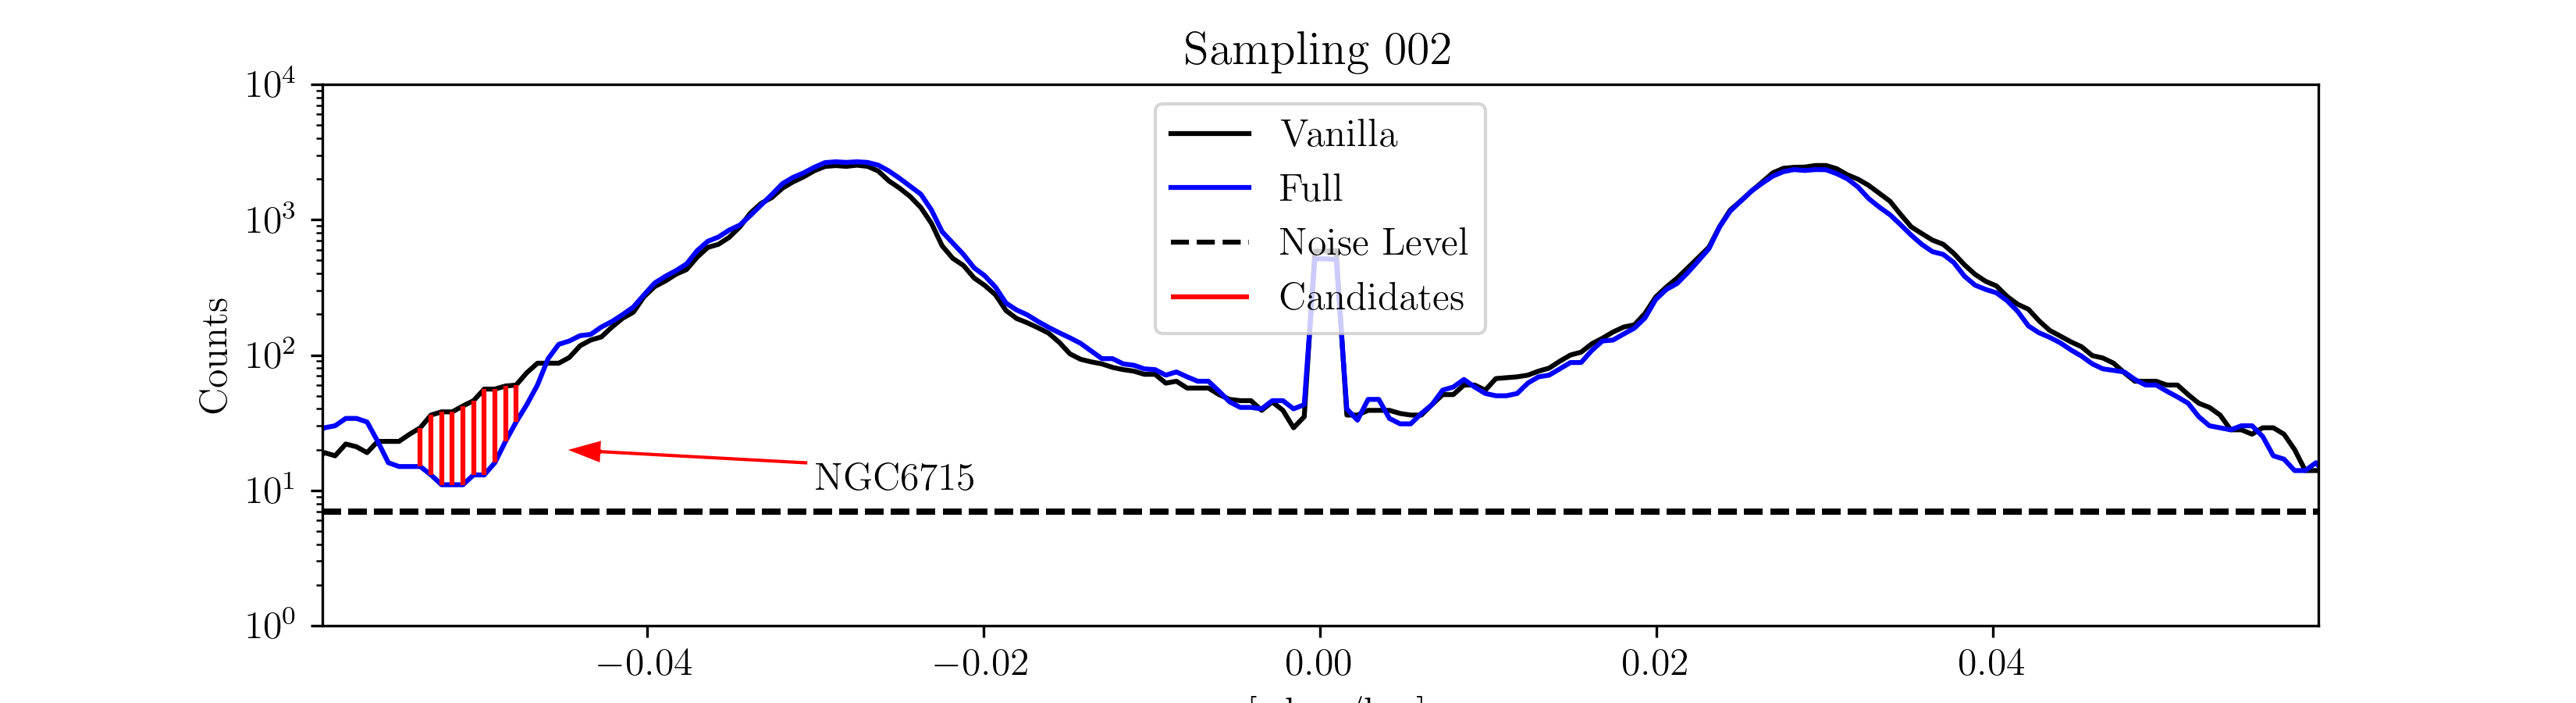
\includegraphics[width=\linewidth]{tau-profile-monte-carlo-002.png}
      \caption{Gap Gallery}
      \label{fig:gallery0}
      \end{figure*}    


    \begin{figure*}
      \centering
      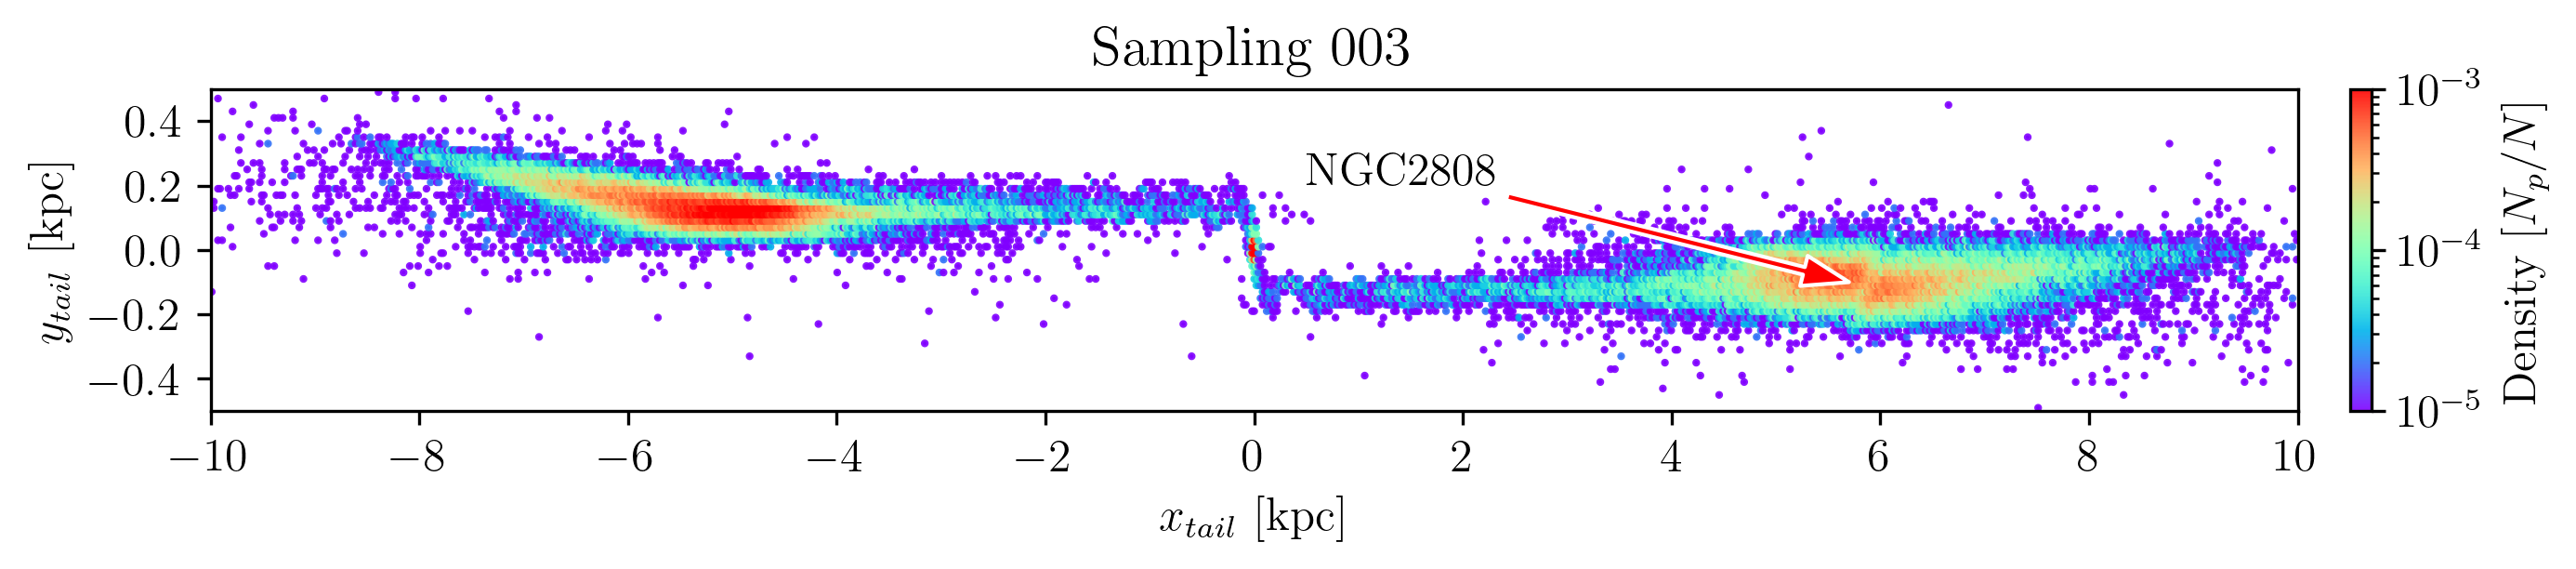
\includegraphics[width=\linewidth]{gallery_of_gaps_monte-carlo-003.png}      
      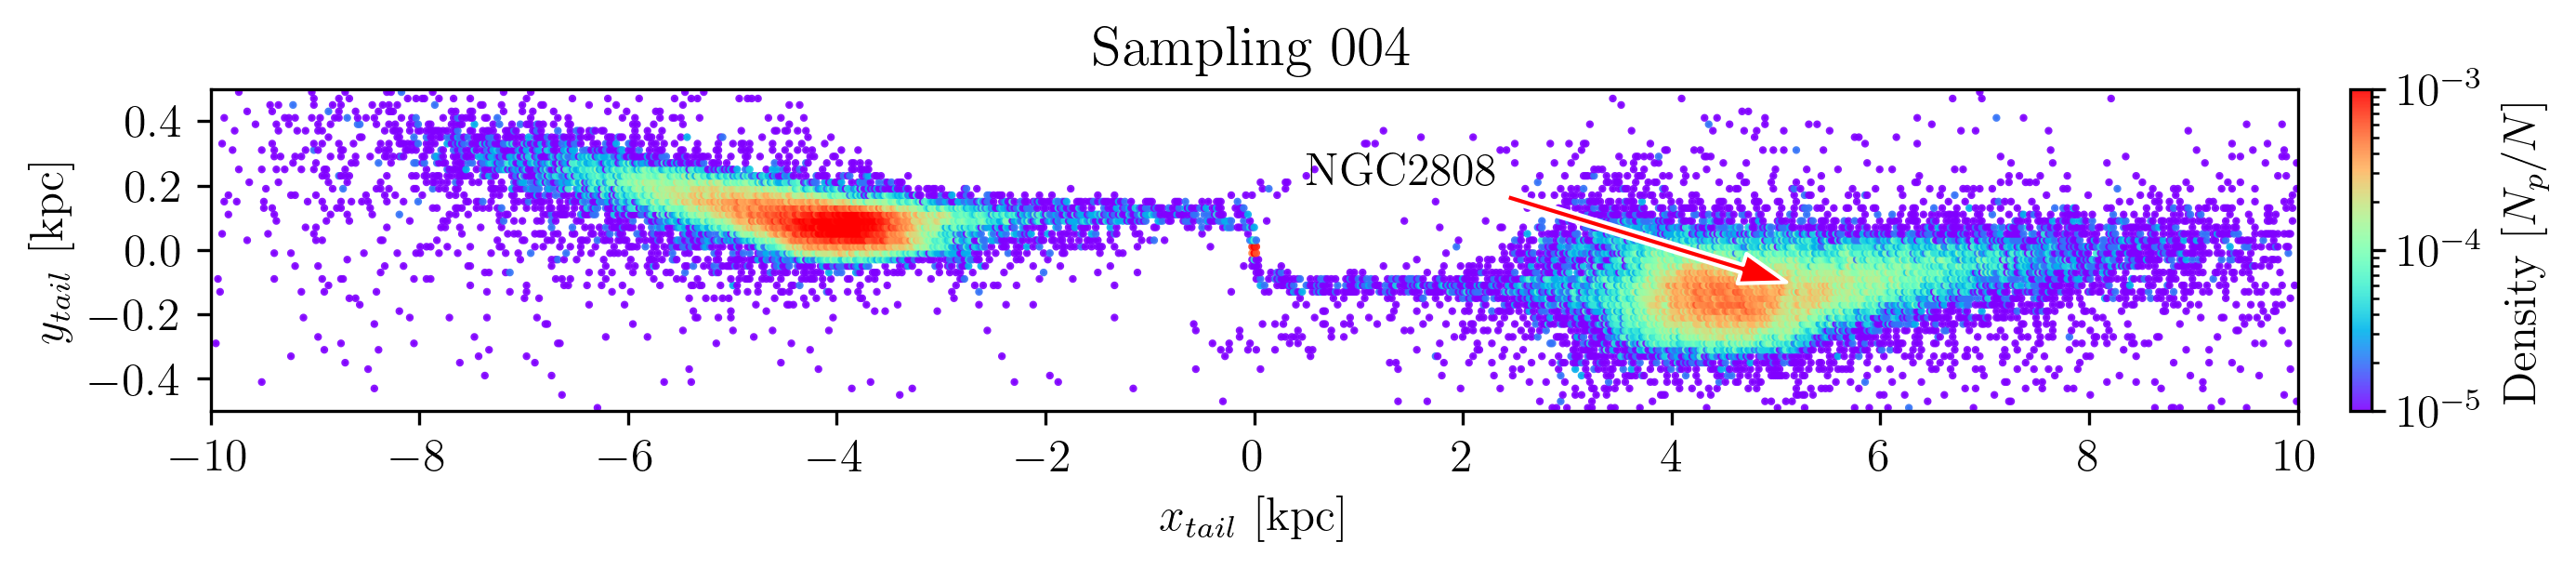
\includegraphics[width=\linewidth]{gallery_of_gaps_monte-carlo-004.png}
      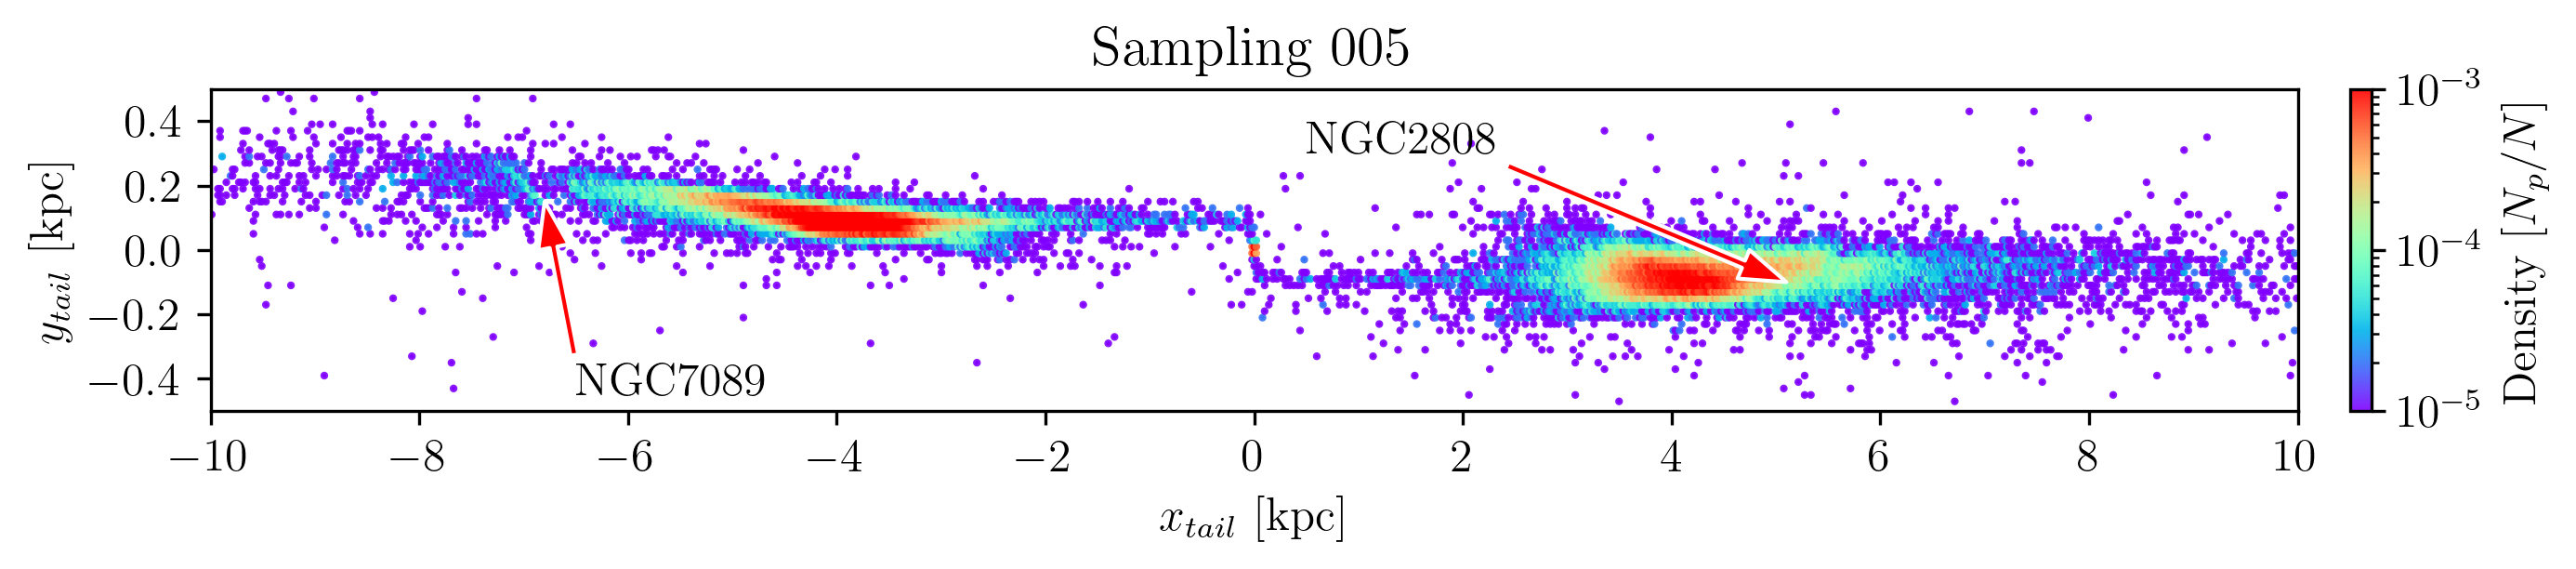
\includegraphics[width=\linewidth]{gallery_of_gaps_monte-carlo-005.png}
      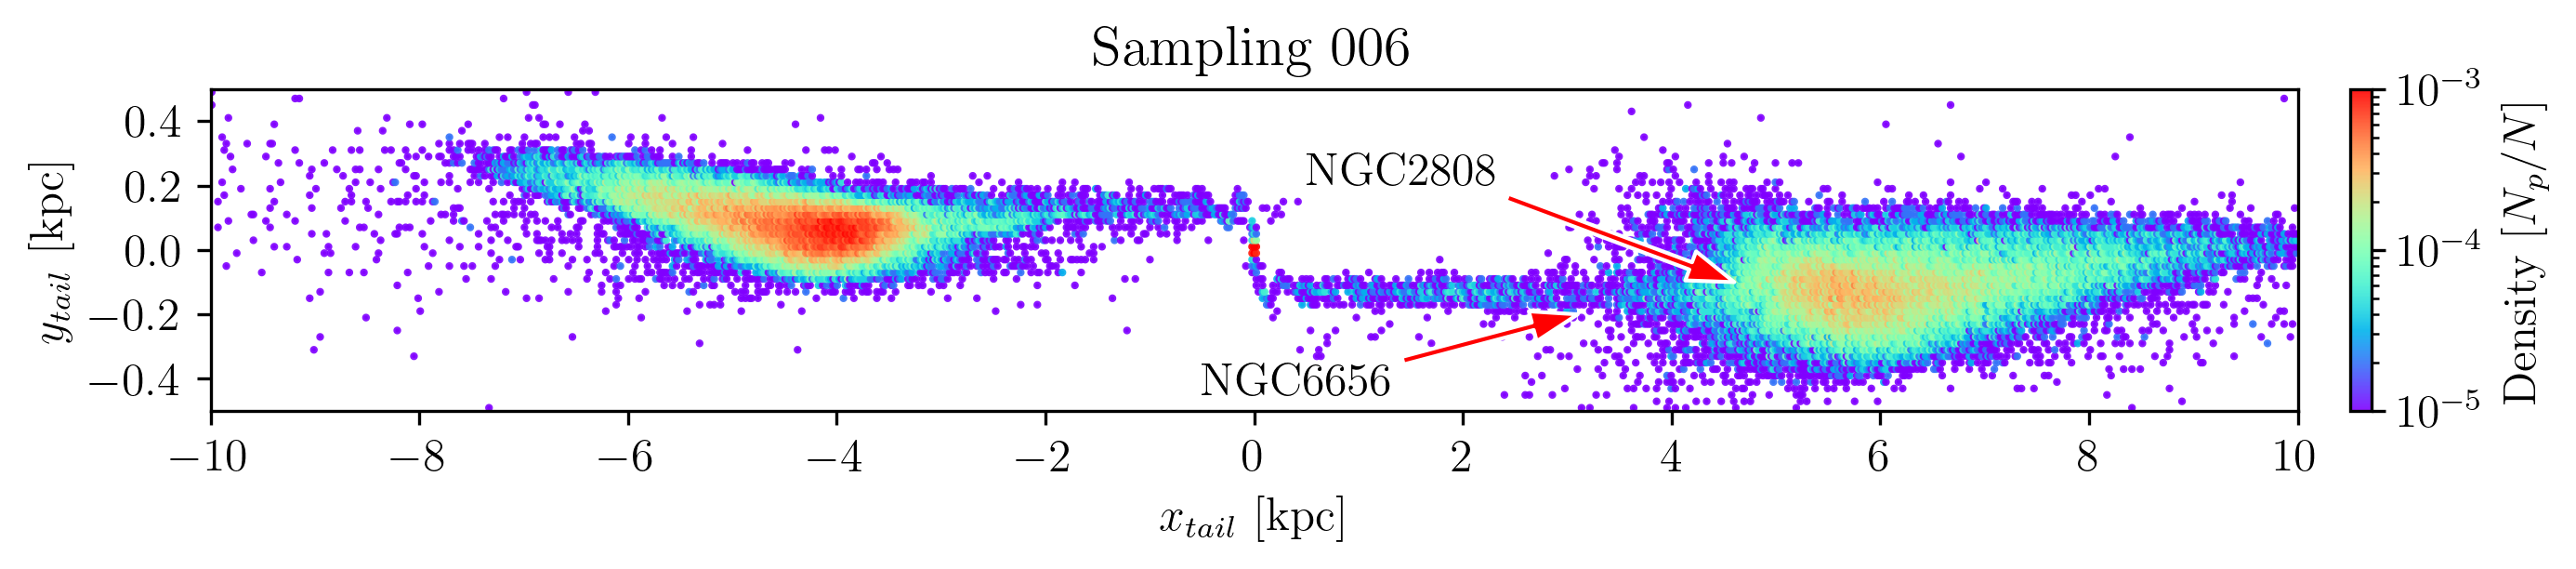
\includegraphics[width=\linewidth]{gallery_of_gaps_monte-carlo-006.png}
      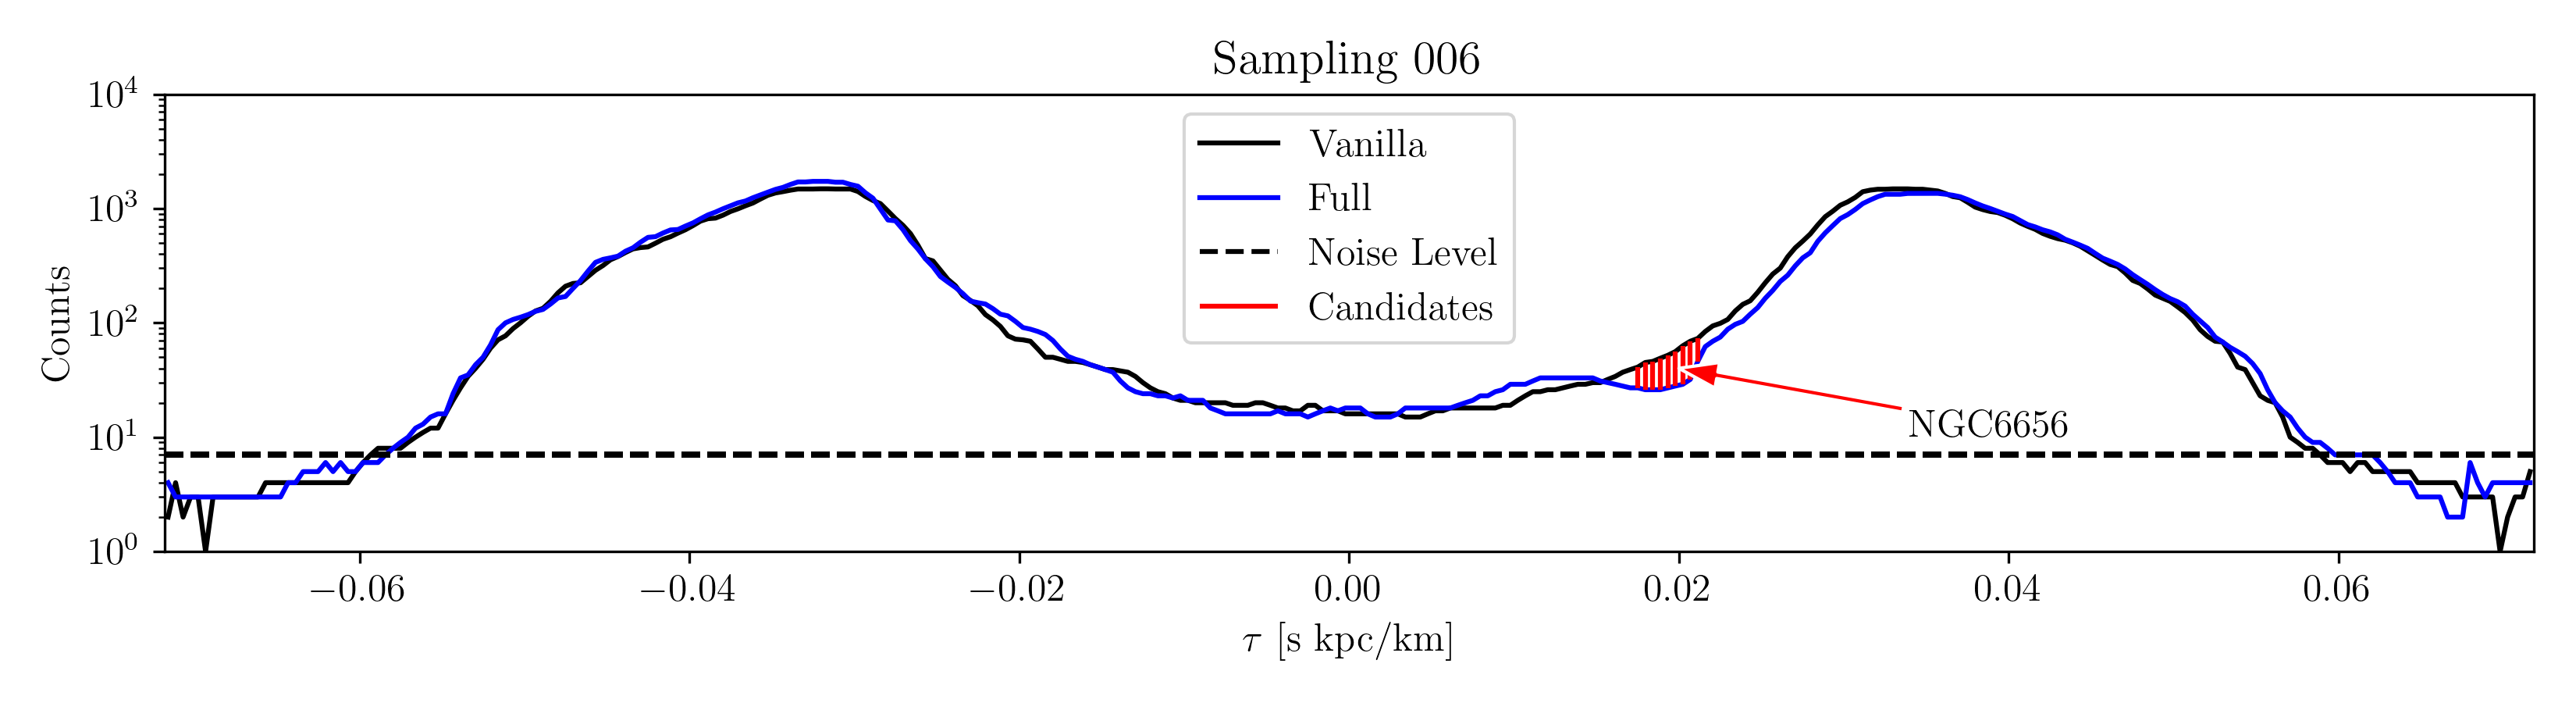
\includegraphics[width=\linewidth]{tau-profile-monte-carlo-006.png}
      \caption{Gap Gallery}
      \label{fig:gallery1}
      \end{figure*}        


    \begin{figure*}
      \centering
      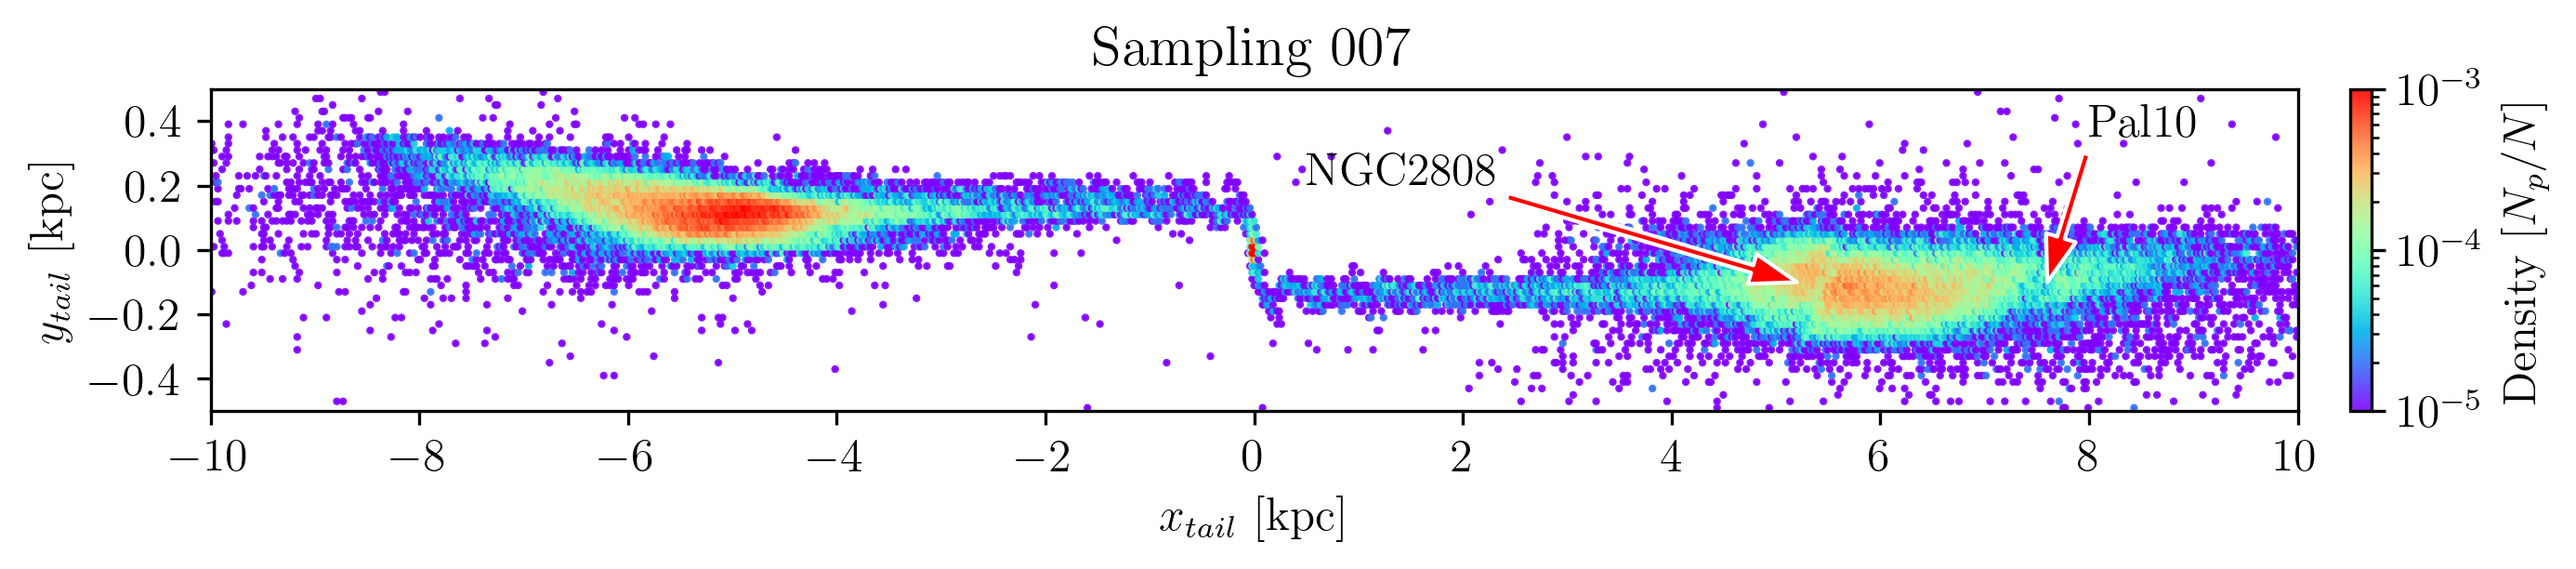
\includegraphics[width=\linewidth]{gallery_of_gaps_monte-carlo-007.png}
      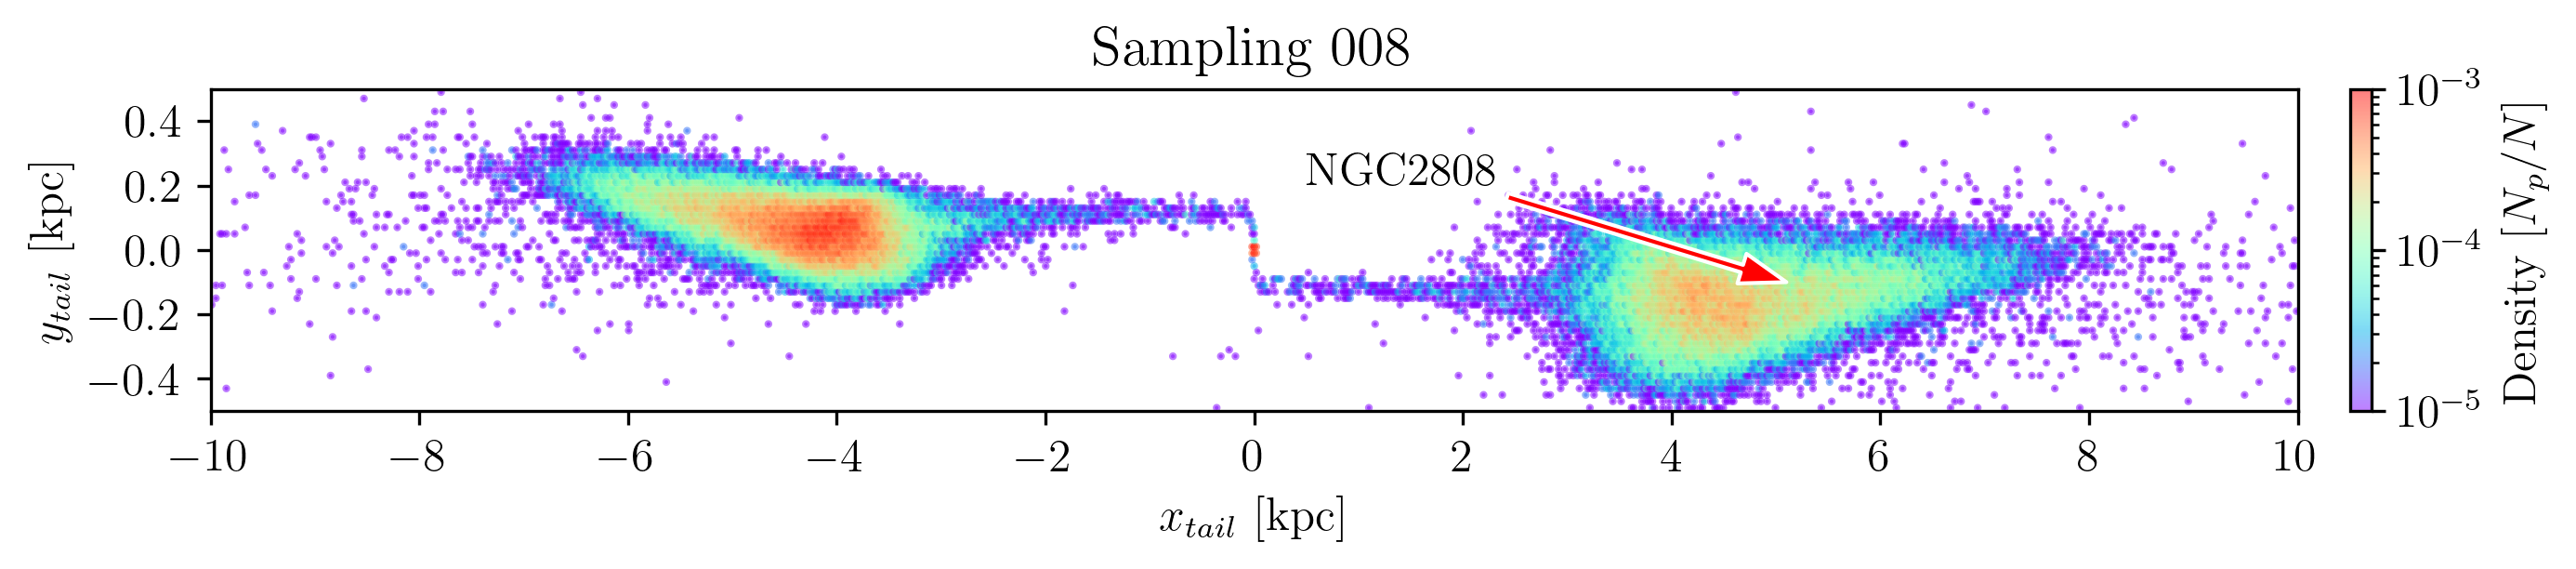
\includegraphics[width=\linewidth]{gallery_of_gaps_monte-carlo-008.png}
      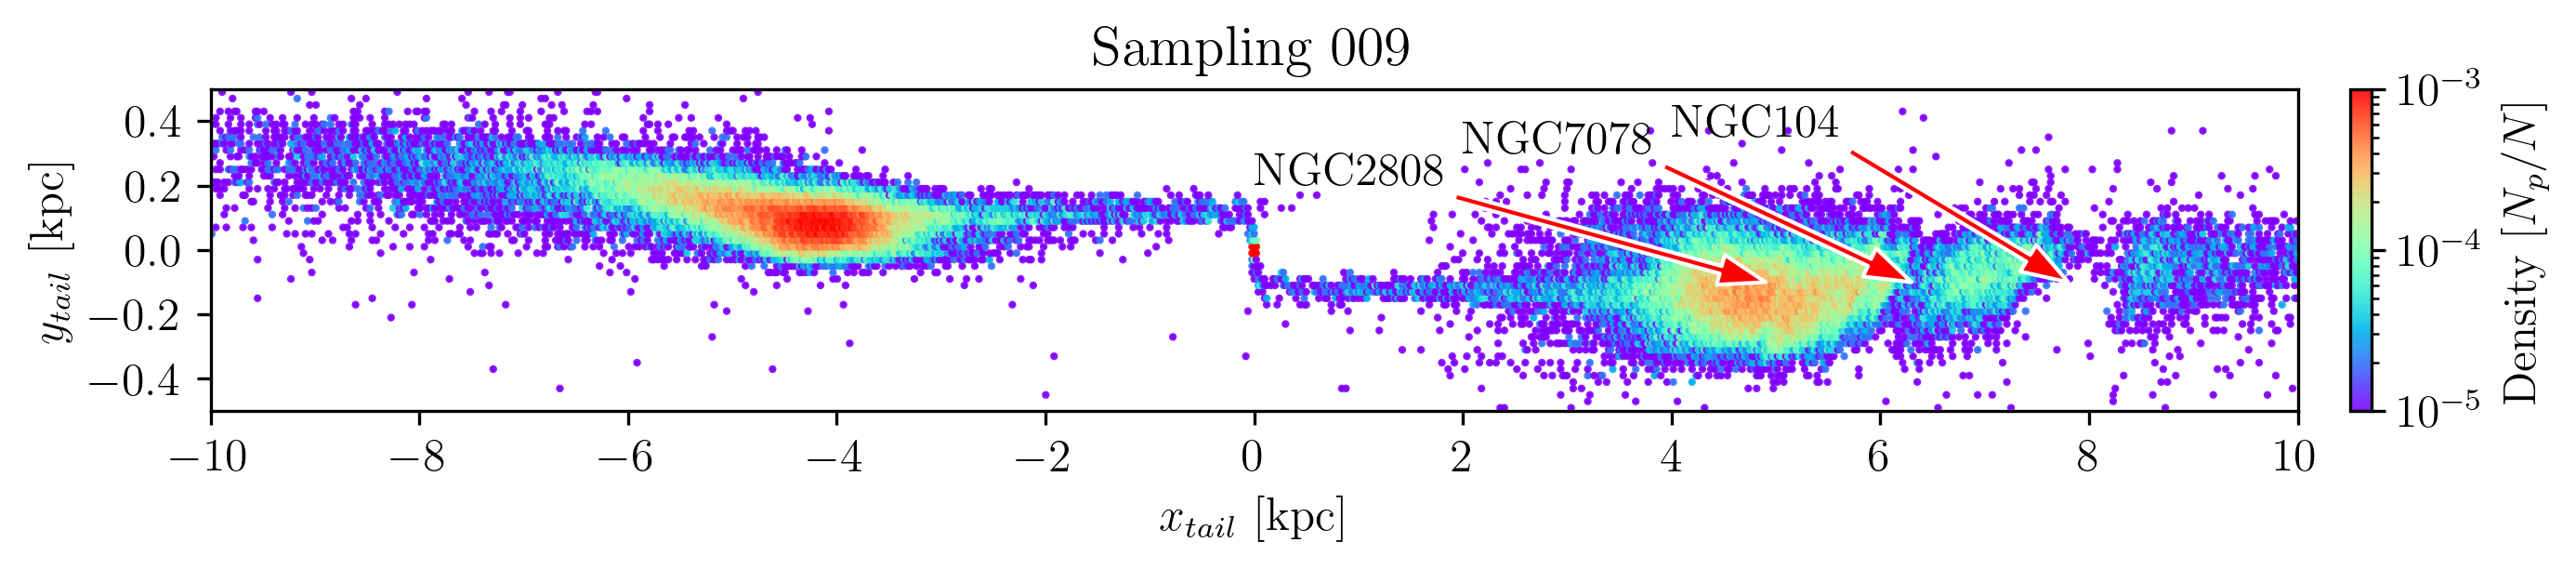
\includegraphics[width=\linewidth]{gallery_of_gaps_monte-carlo-009.png}      
      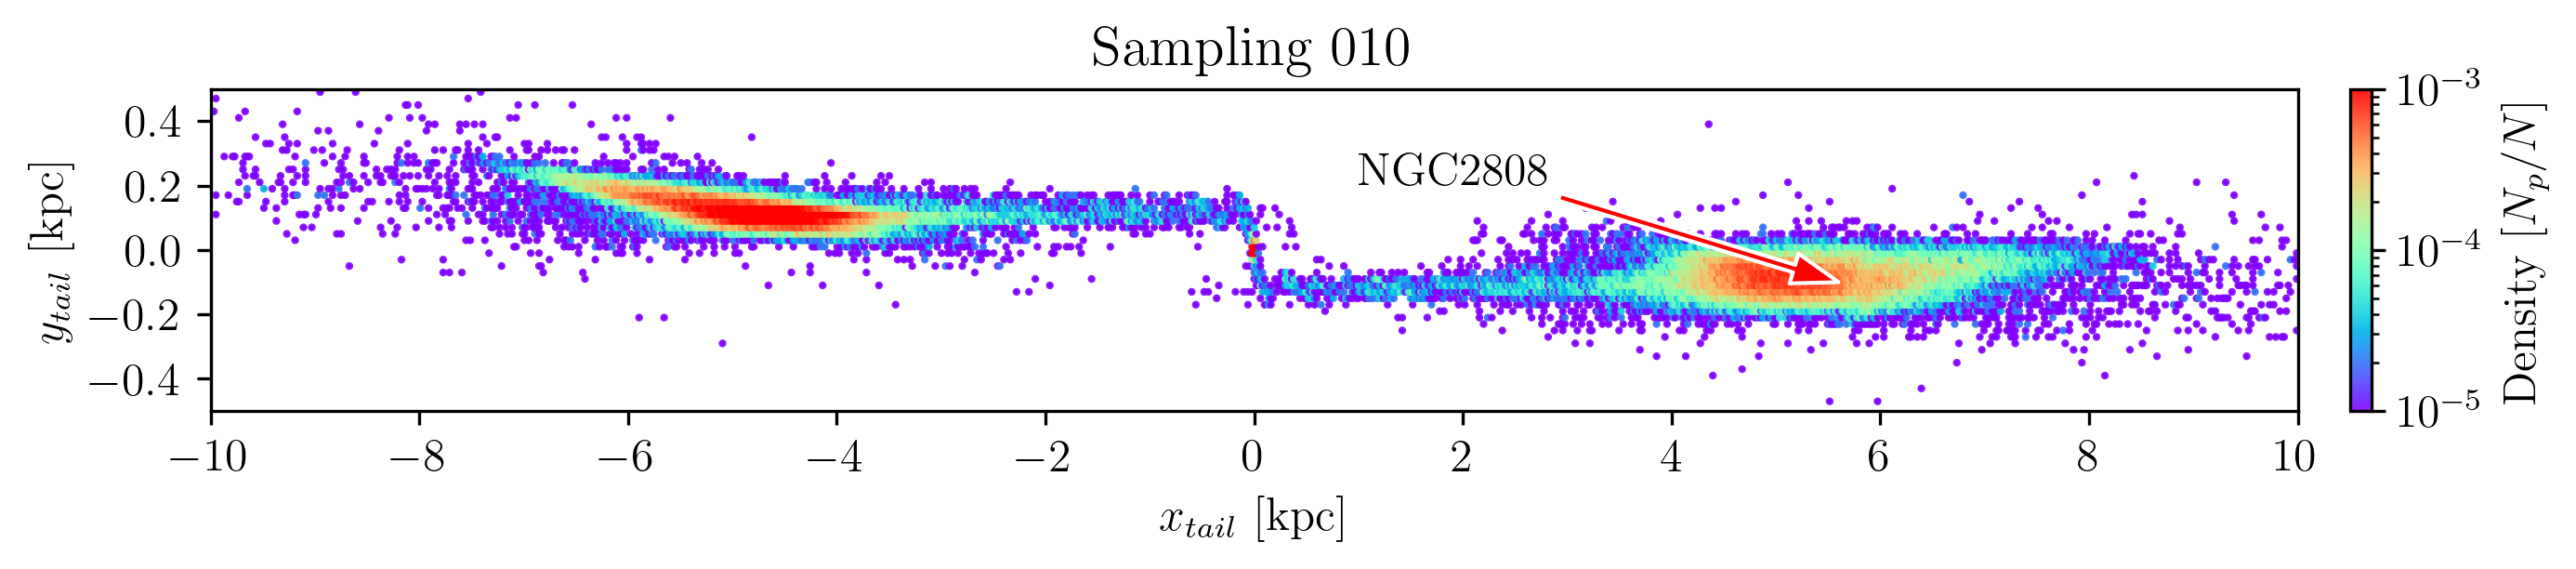
\includegraphics[width=\linewidth]{gallery_of_gaps_monte-carlo-010.png}
      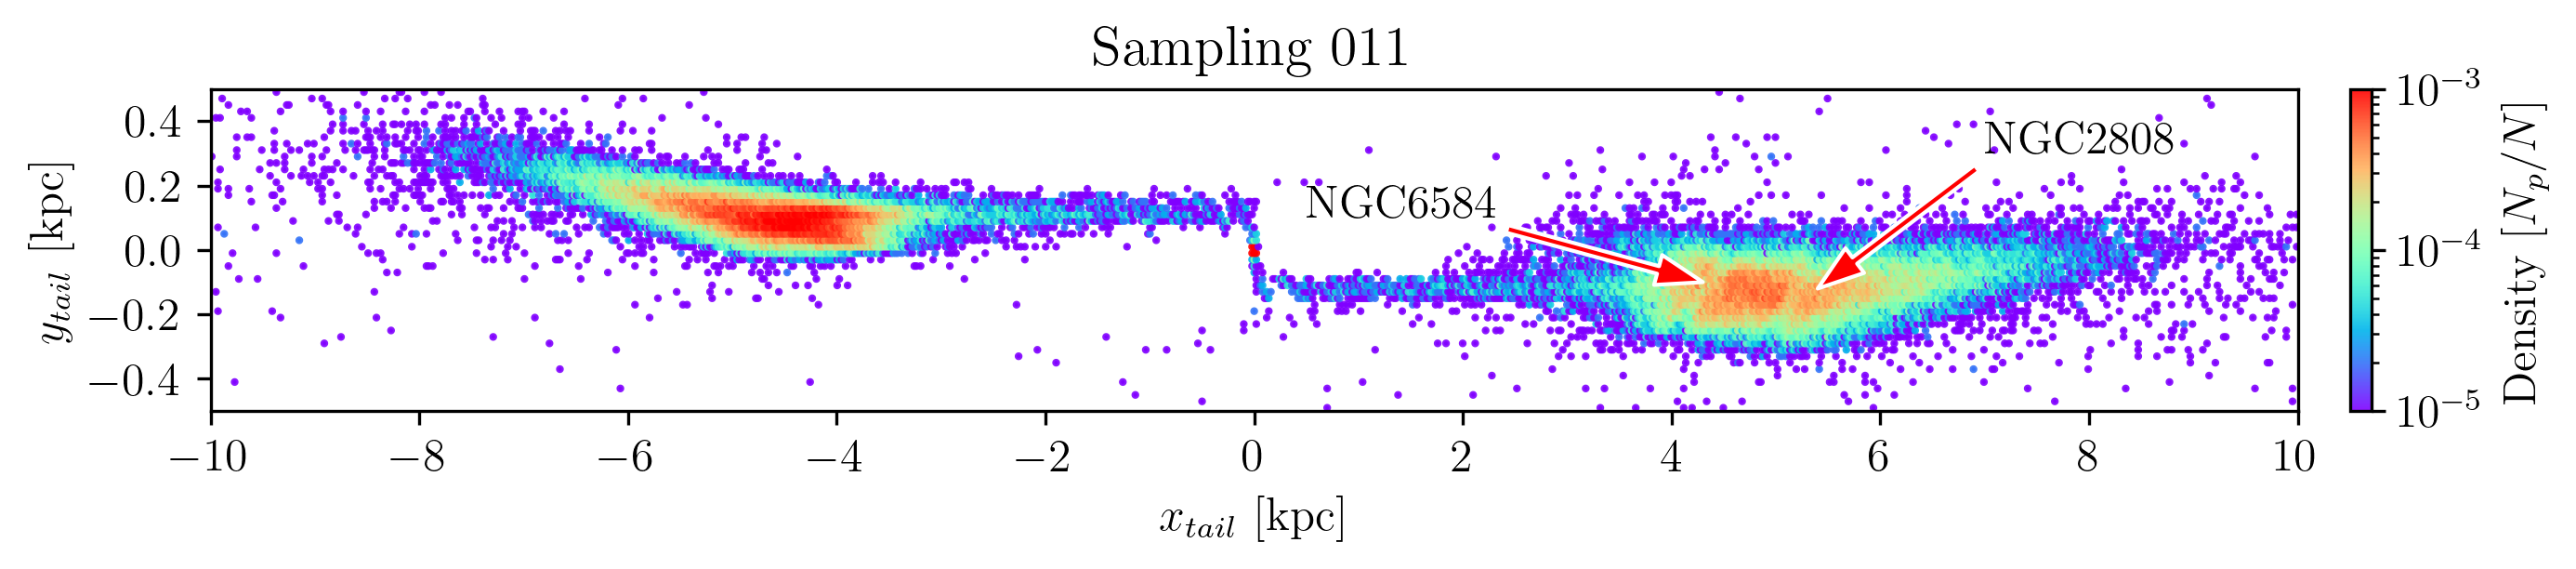
\includegraphics[width=\linewidth]{gallery_of_gaps_monte-carlo-011.png}
      \caption{Gap Gallery}
      \label{fig:gallery2}
      \end{figure*}        


    \begin{figure*}
      \centering
      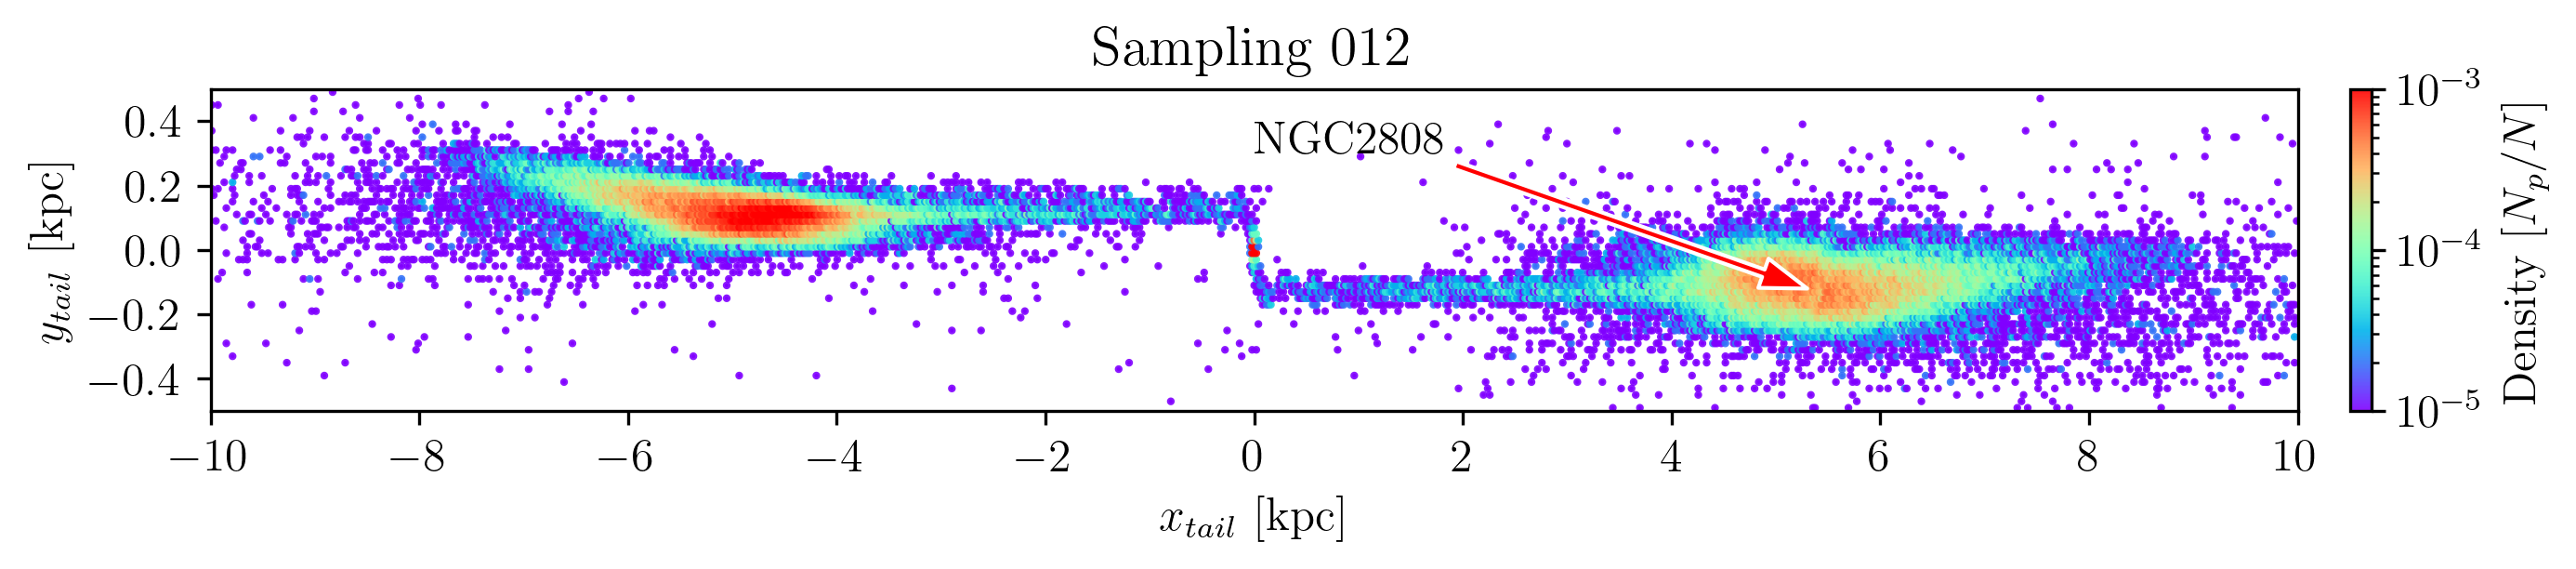
\includegraphics[width=\linewidth]{gallery_of_gaps_monte-carlo-012.png}
      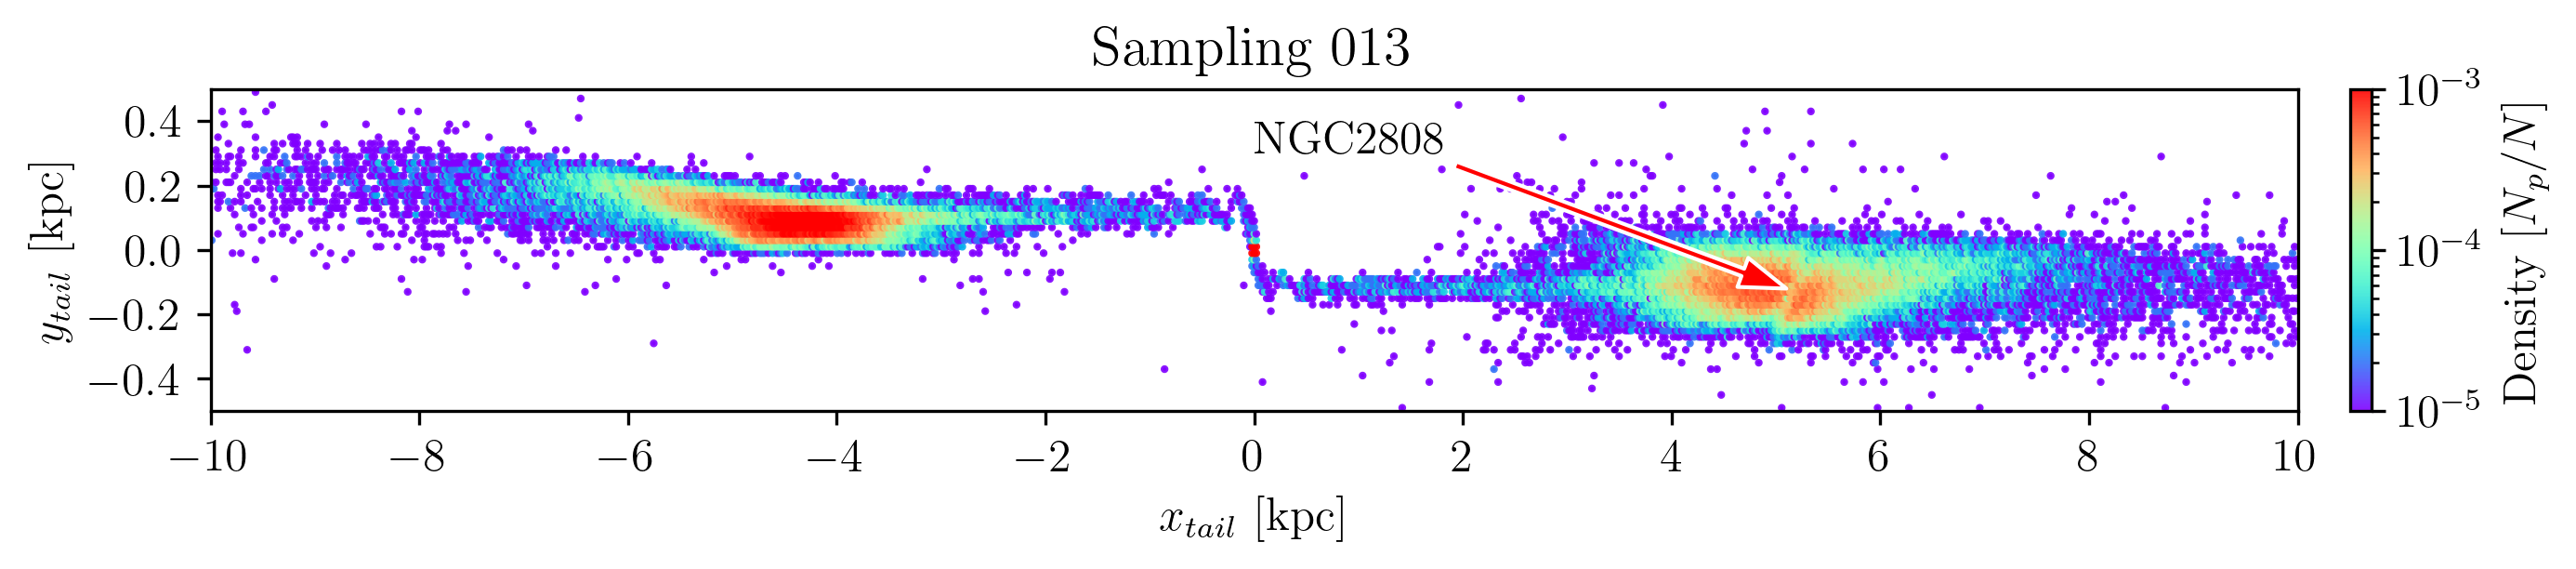
\includegraphics[width=\linewidth]{gallery_of_gaps_monte-carlo-013.png}
      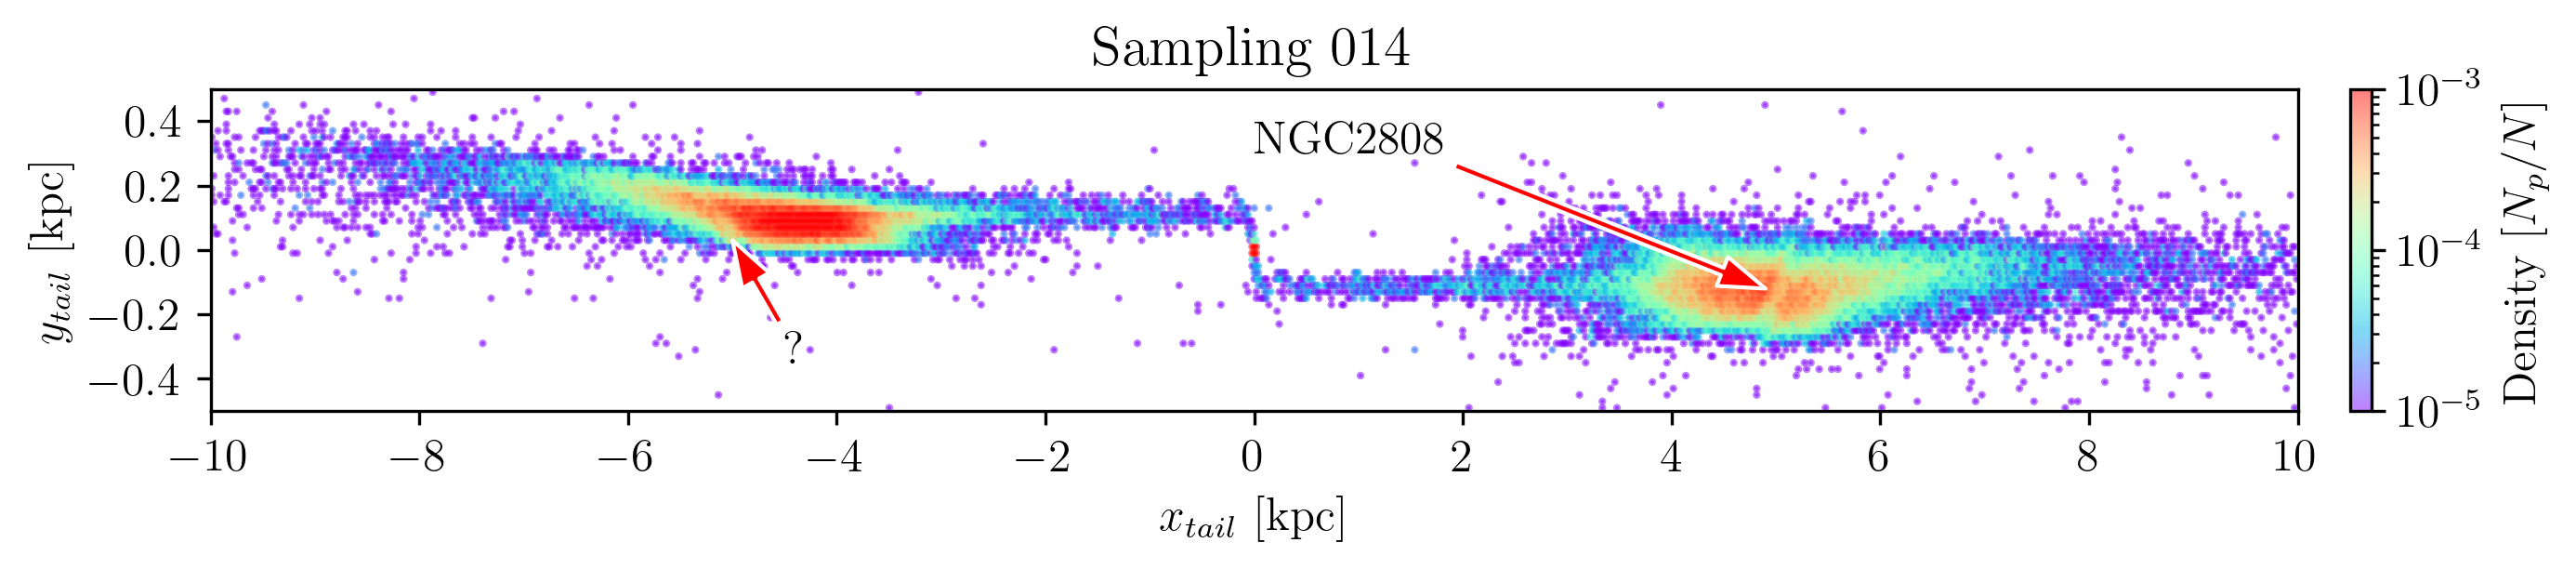
\includegraphics[width=\linewidth]{gallery_of_gaps_monte-carlo-014.png}      
      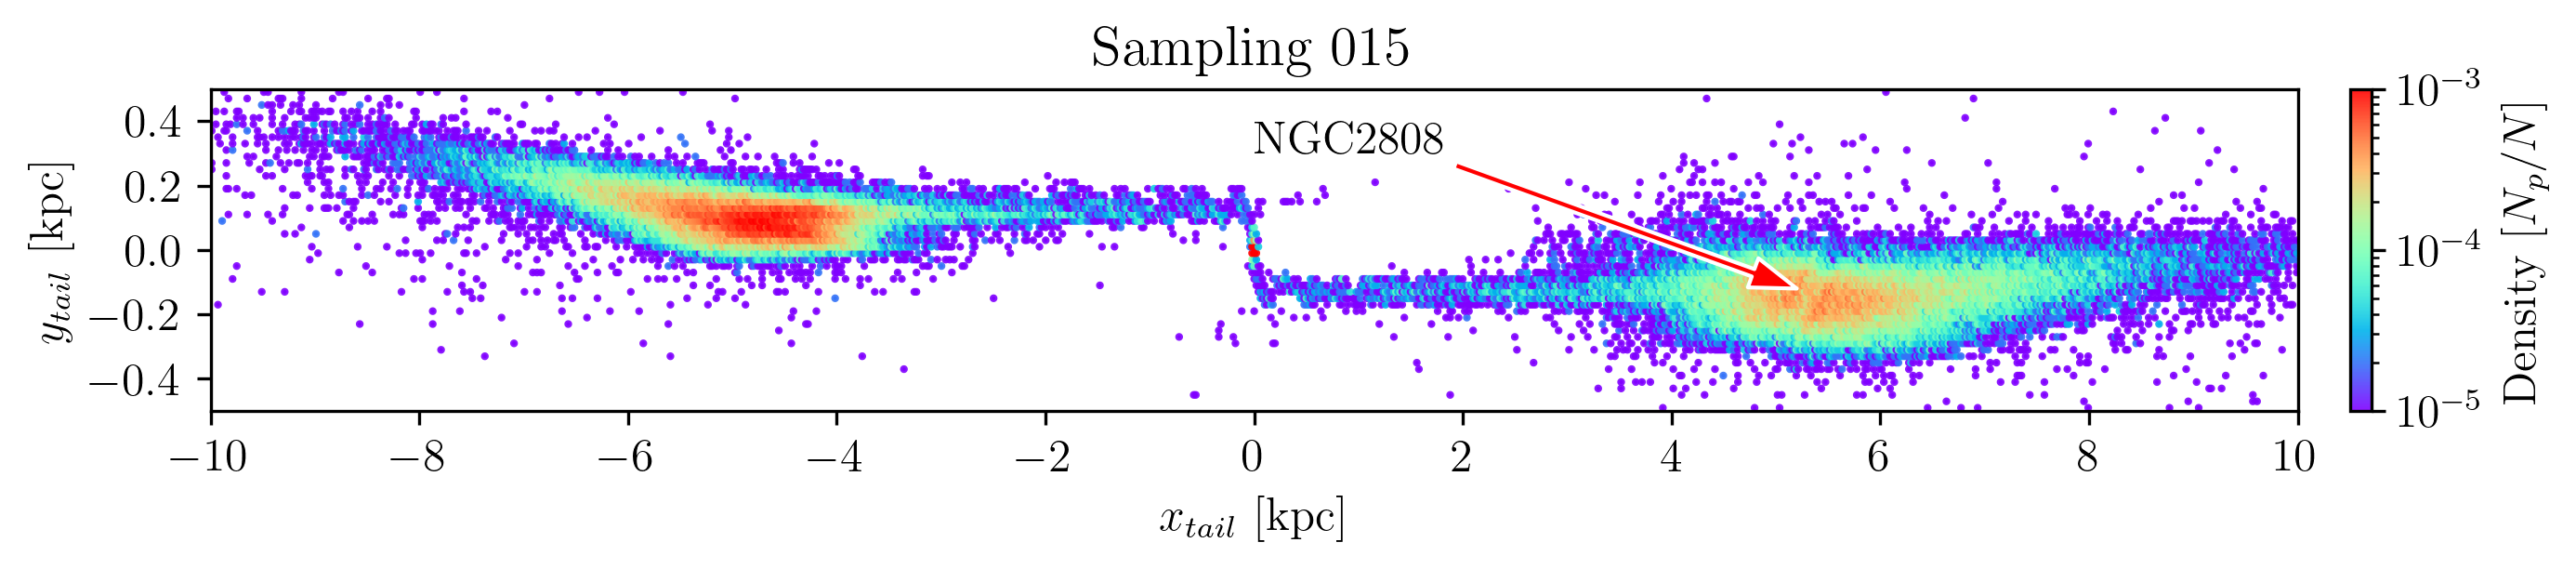
\includegraphics[width=\linewidth]{gallery_of_gaps_monte-carlo-015.png}
      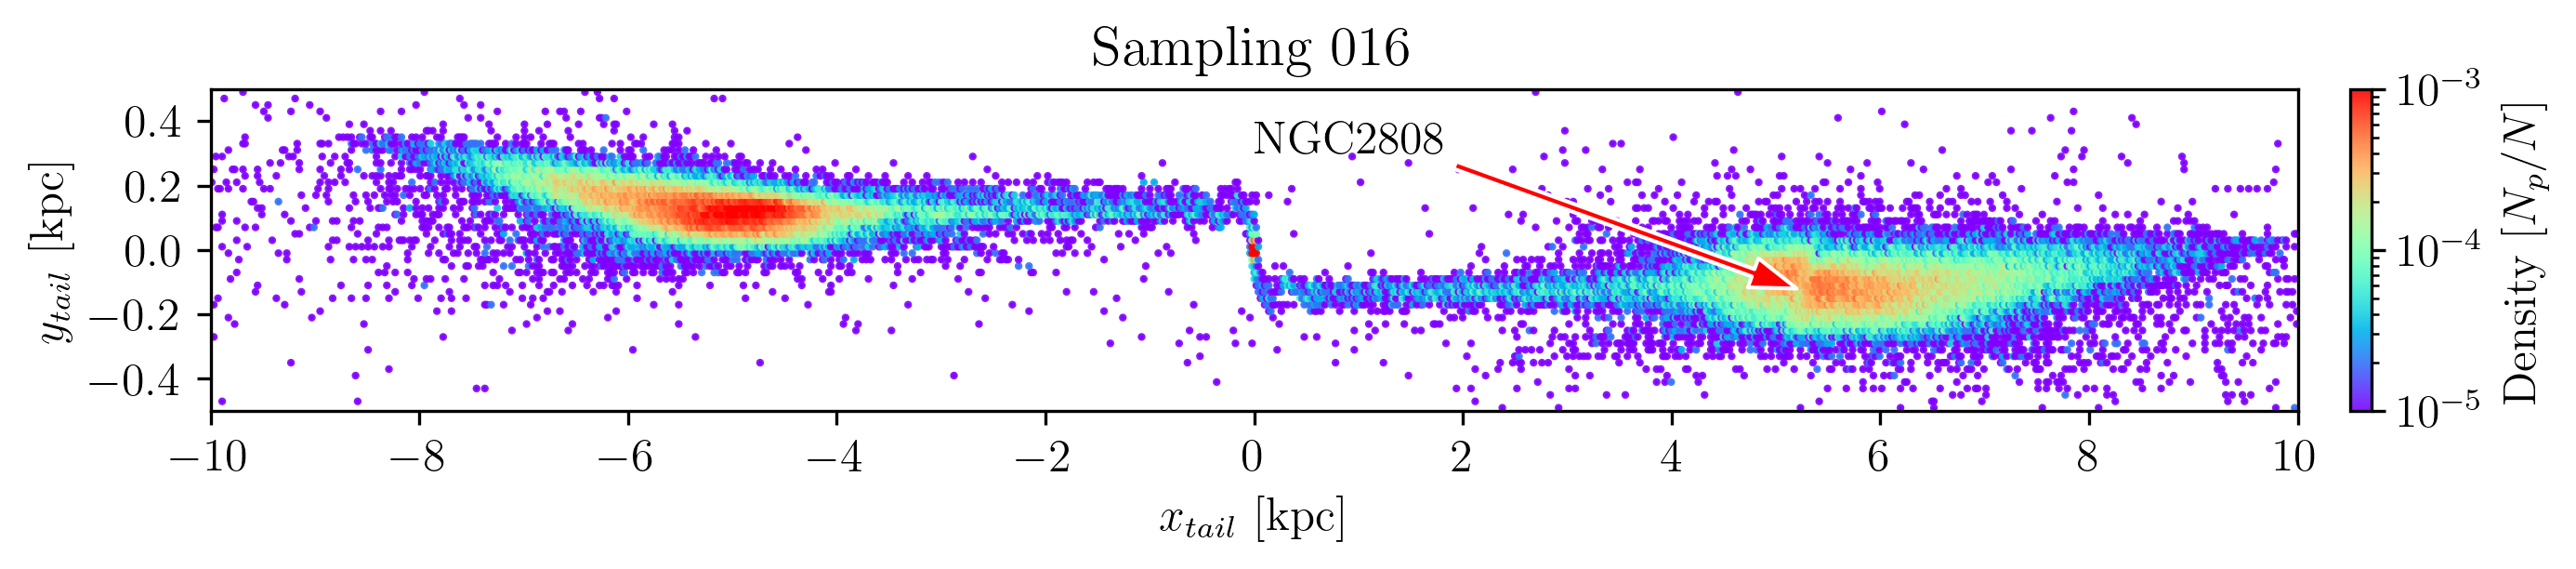
\includegraphics[width=\linewidth]{gallery_of_gaps_monte-carlo-016.png}
      \caption{Gap Gallery}
      \label{fig:gallery3}
      \end{figure*}        

    \begin{figure*}
      \centering
      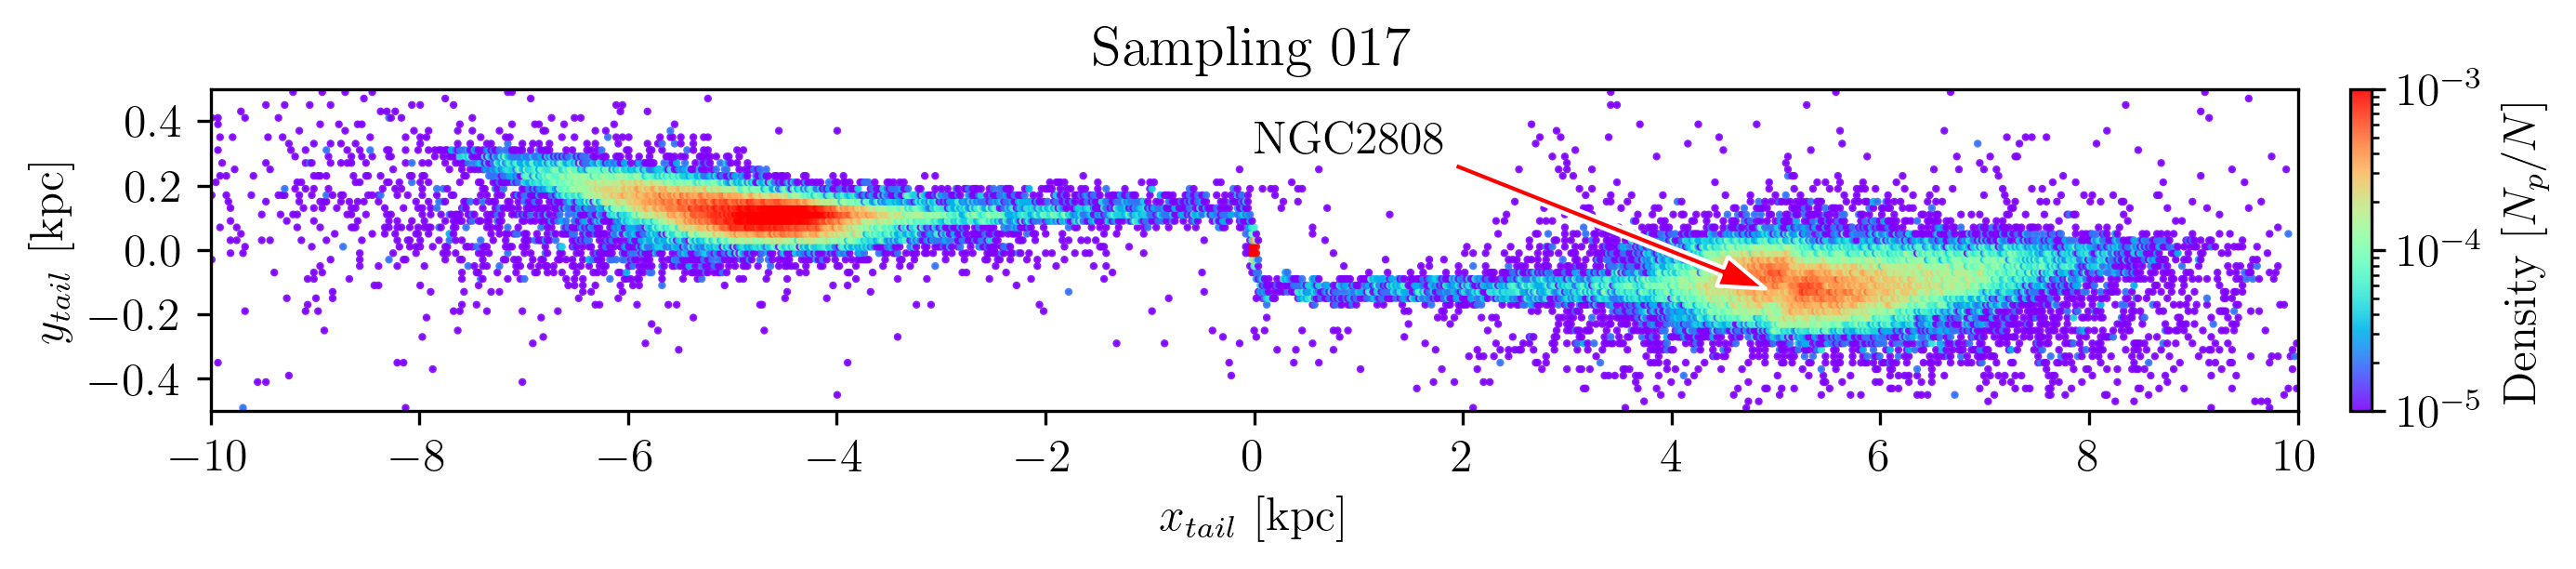
\includegraphics[width=\linewidth]{gallery_of_gaps_monte-carlo-017.png}
      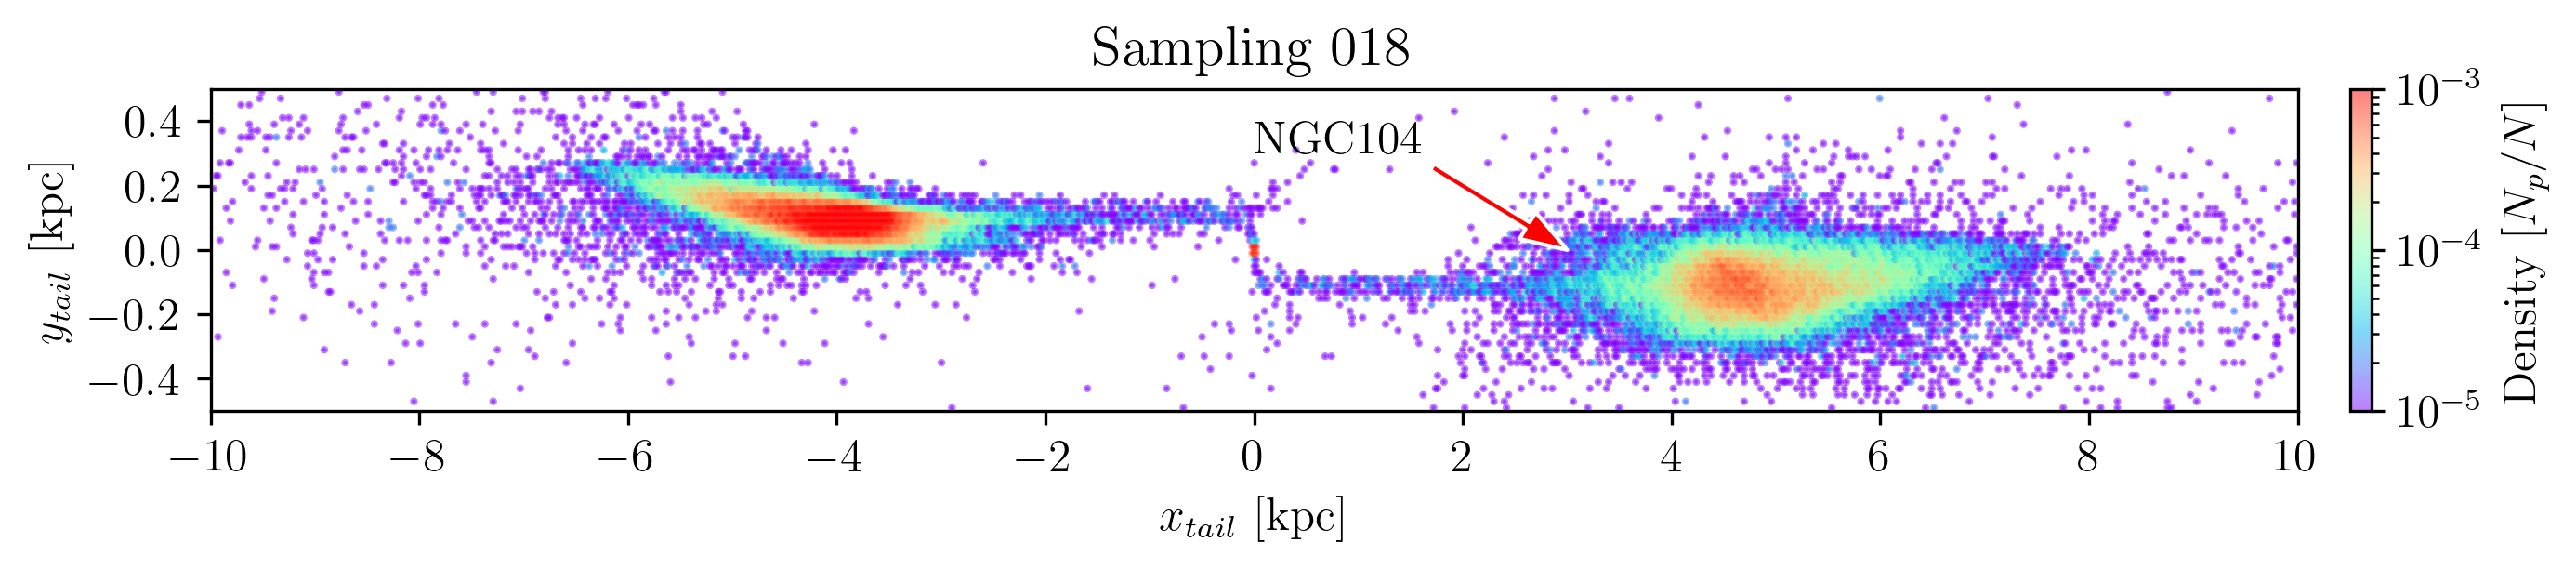
\includegraphics[width=\linewidth]{gallery_of_gaps_monte-carlo-018.png}
      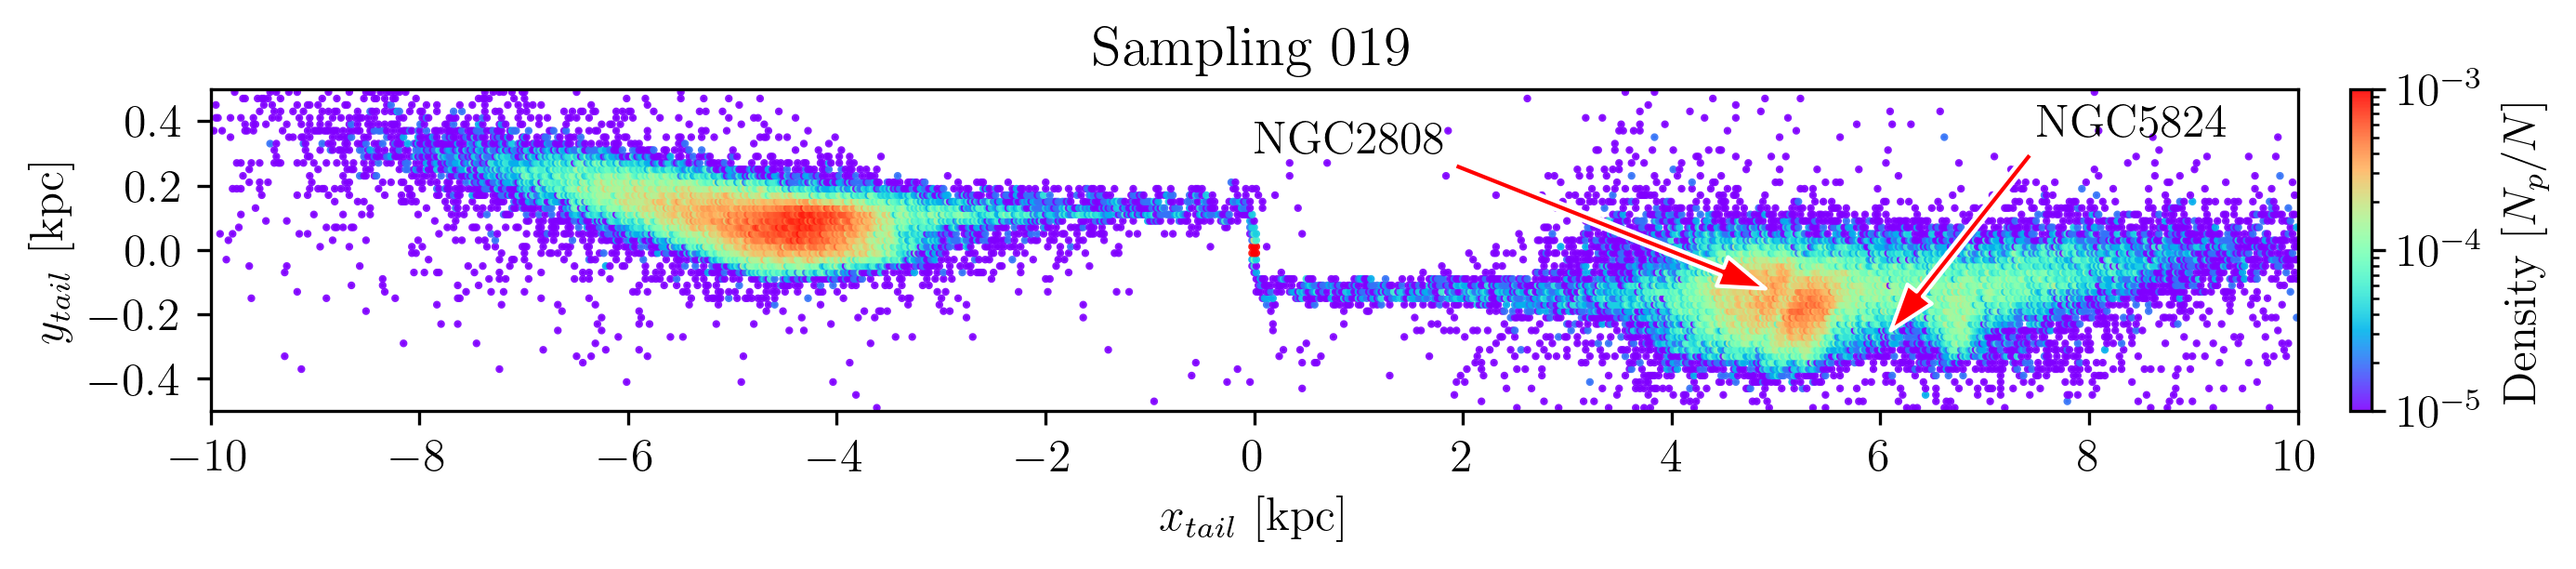
\includegraphics[width=\linewidth]{gallery_of_gaps_monte-carlo-019.png}      
      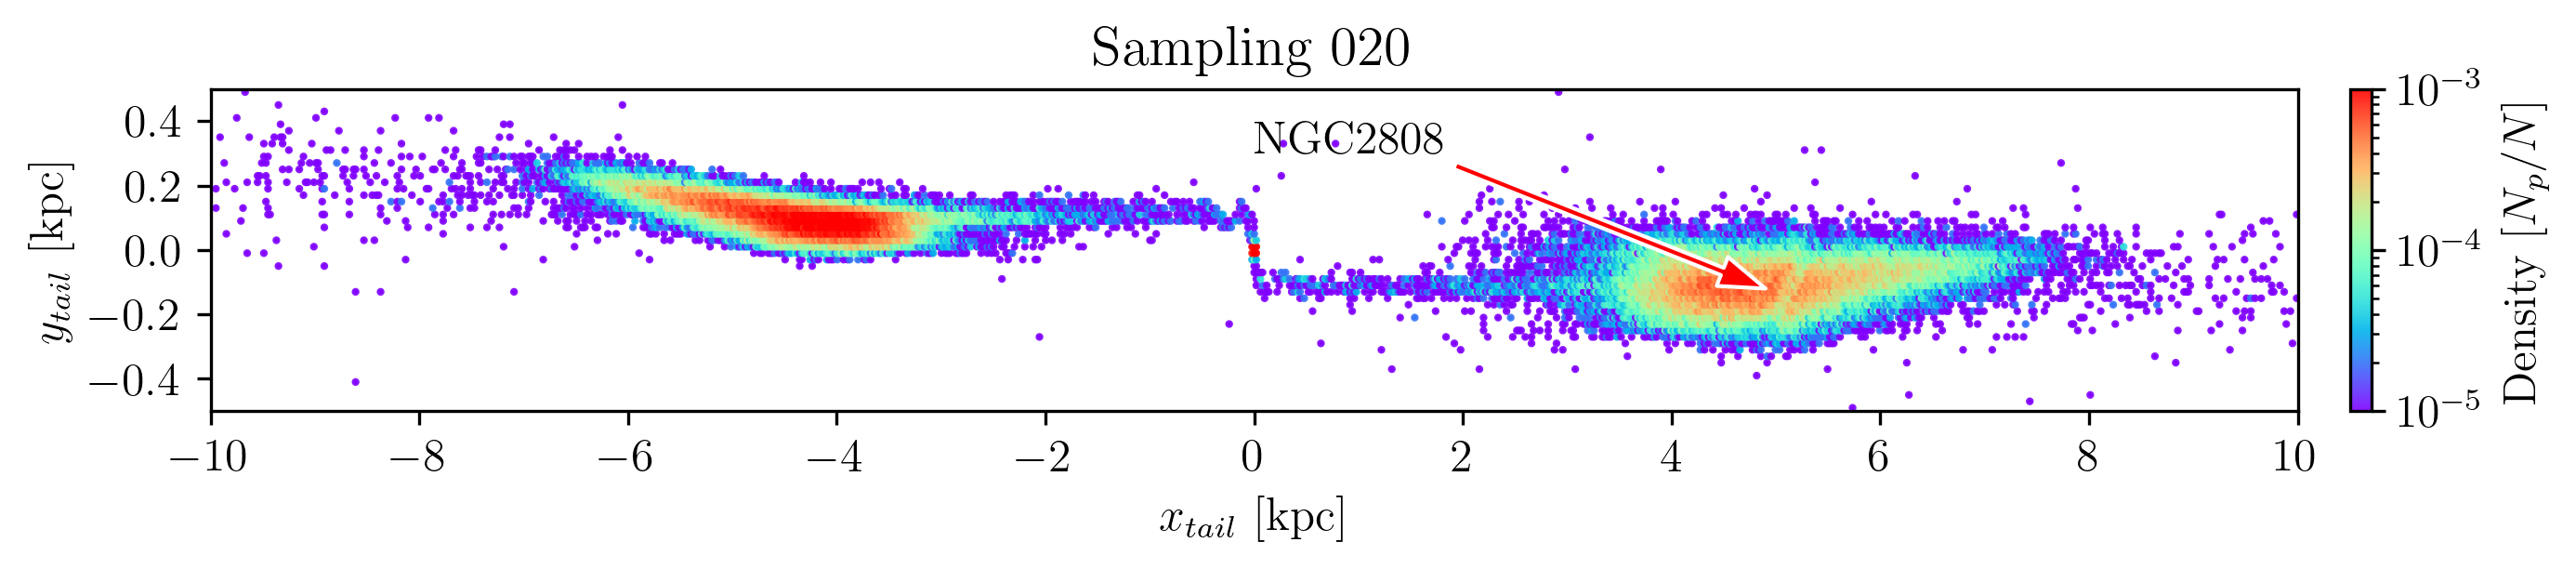
\includegraphics[width=\linewidth]{gallery_of_gaps_monte-carlo-020.png}
      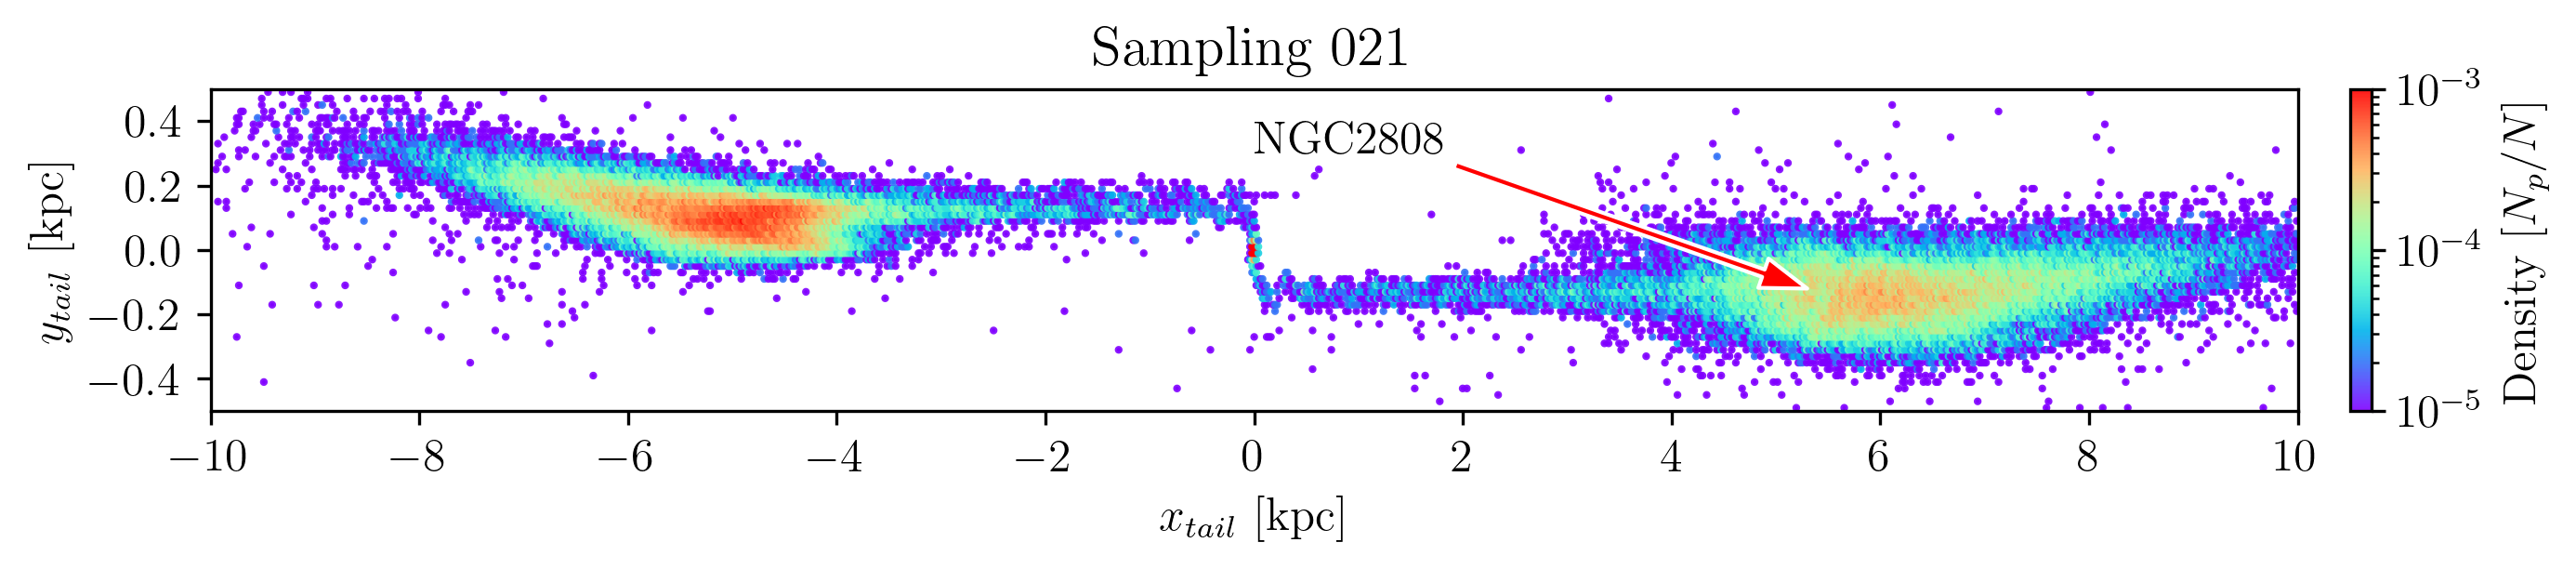
\includegraphics[width=\linewidth]{gallery_of_gaps_monte-carlo-021.png}
      \caption{Gap Gallery}
      \label{fig:gallery4}
      \end{figure*}        

    \begin{figure*}
      \centering
      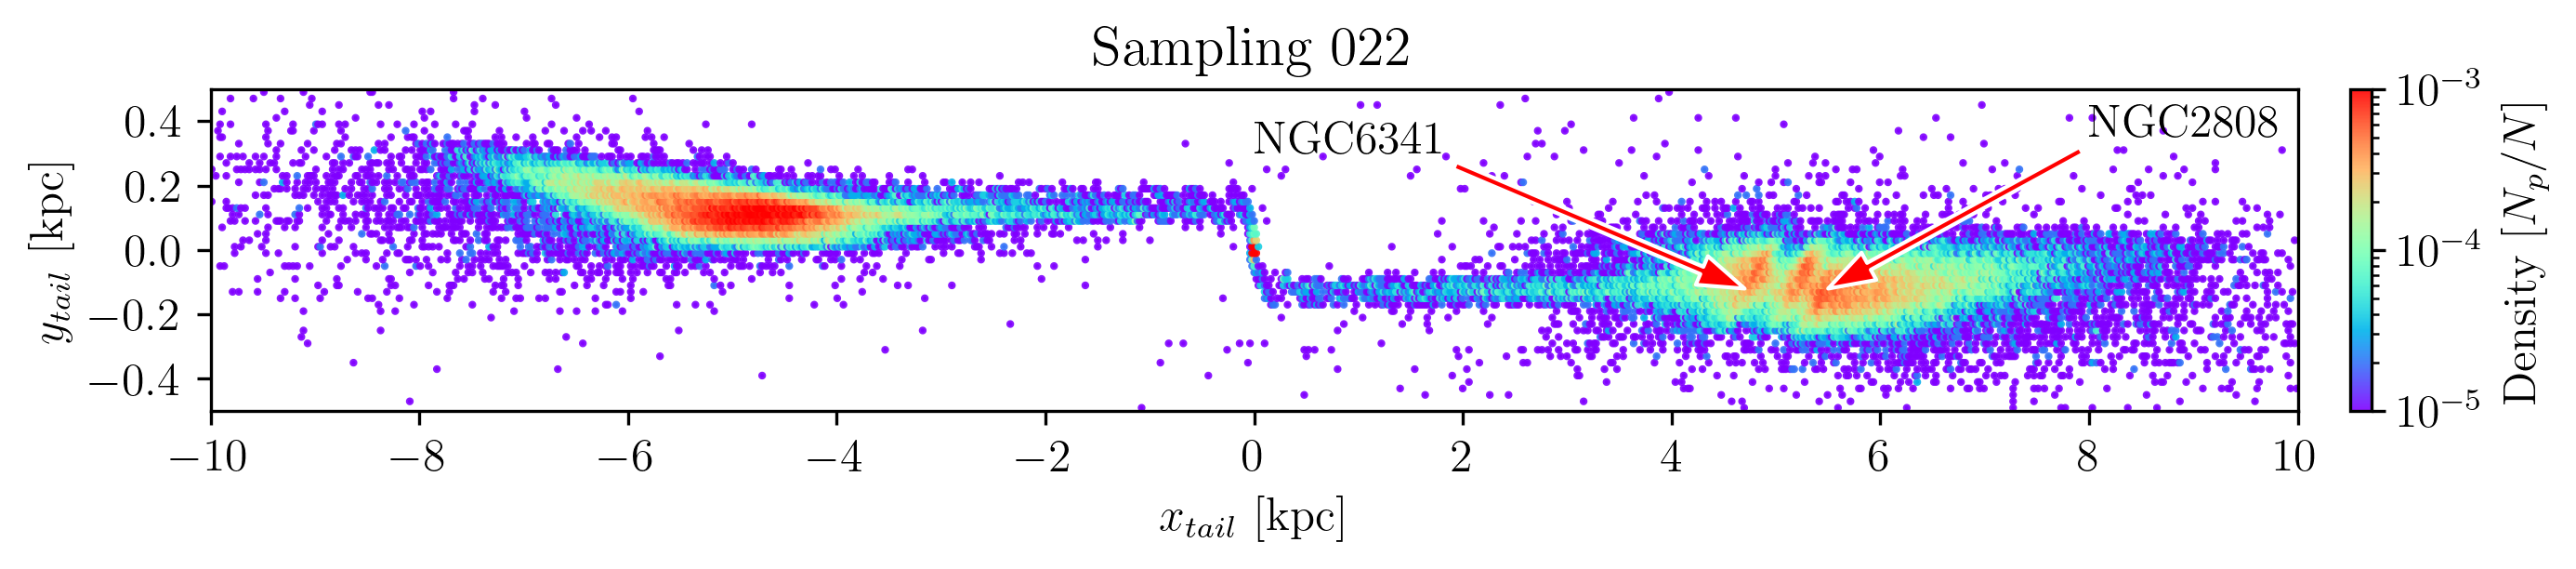
\includegraphics[width=\linewidth]{gallery_of_gaps_monte-carlo-022.png}
      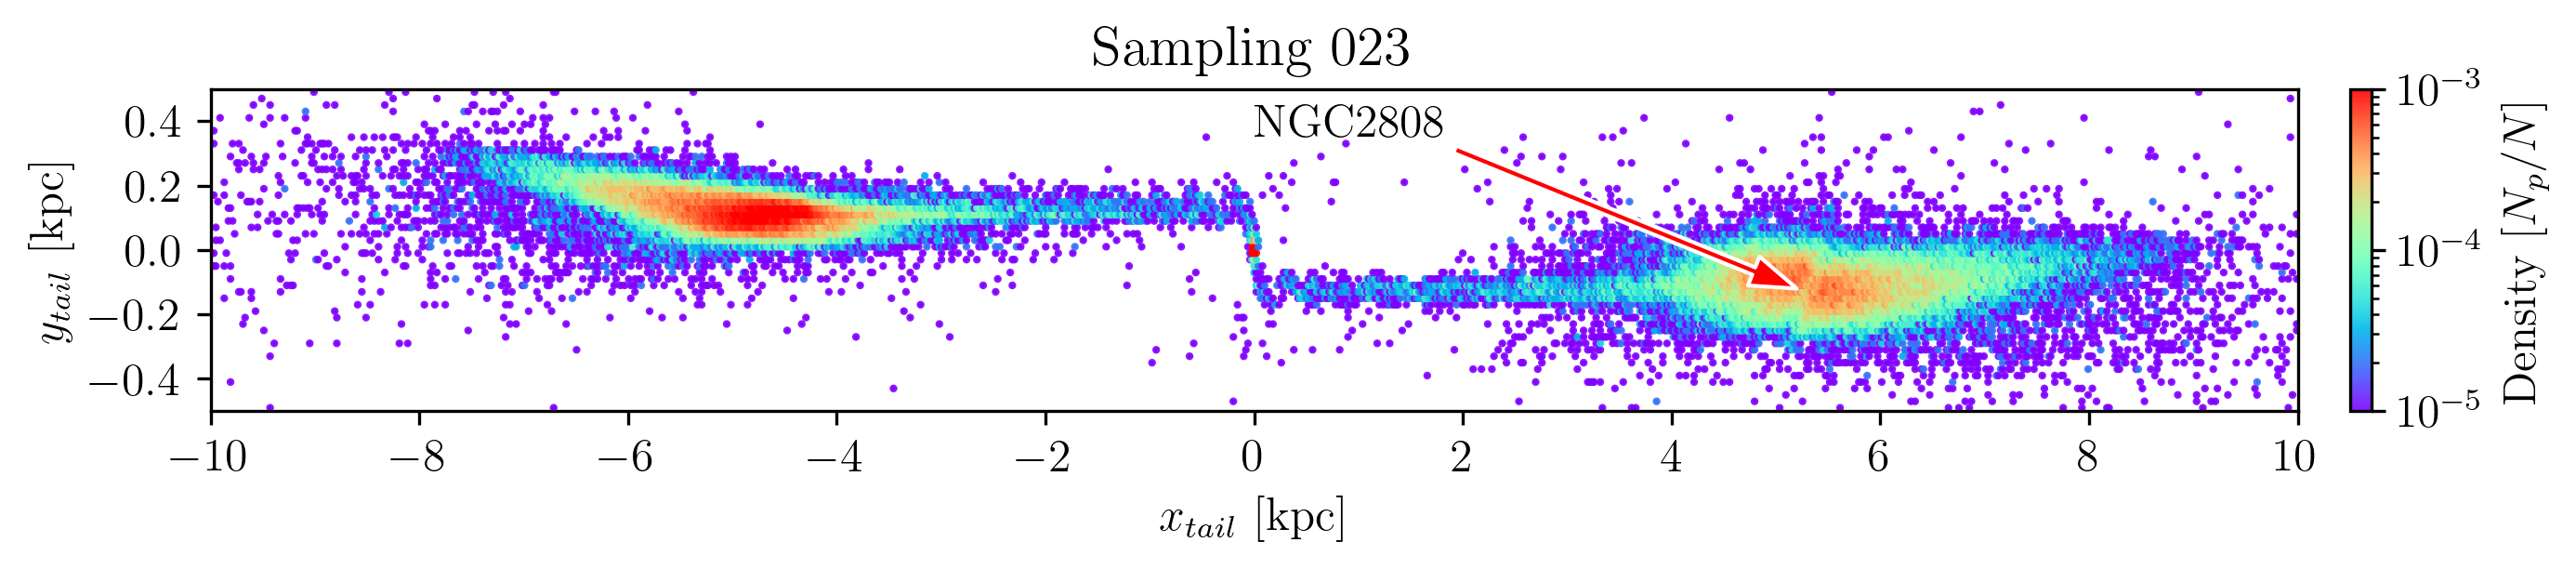
\includegraphics[width=\linewidth]{gallery_of_gaps_monte-carlo-023.png}
      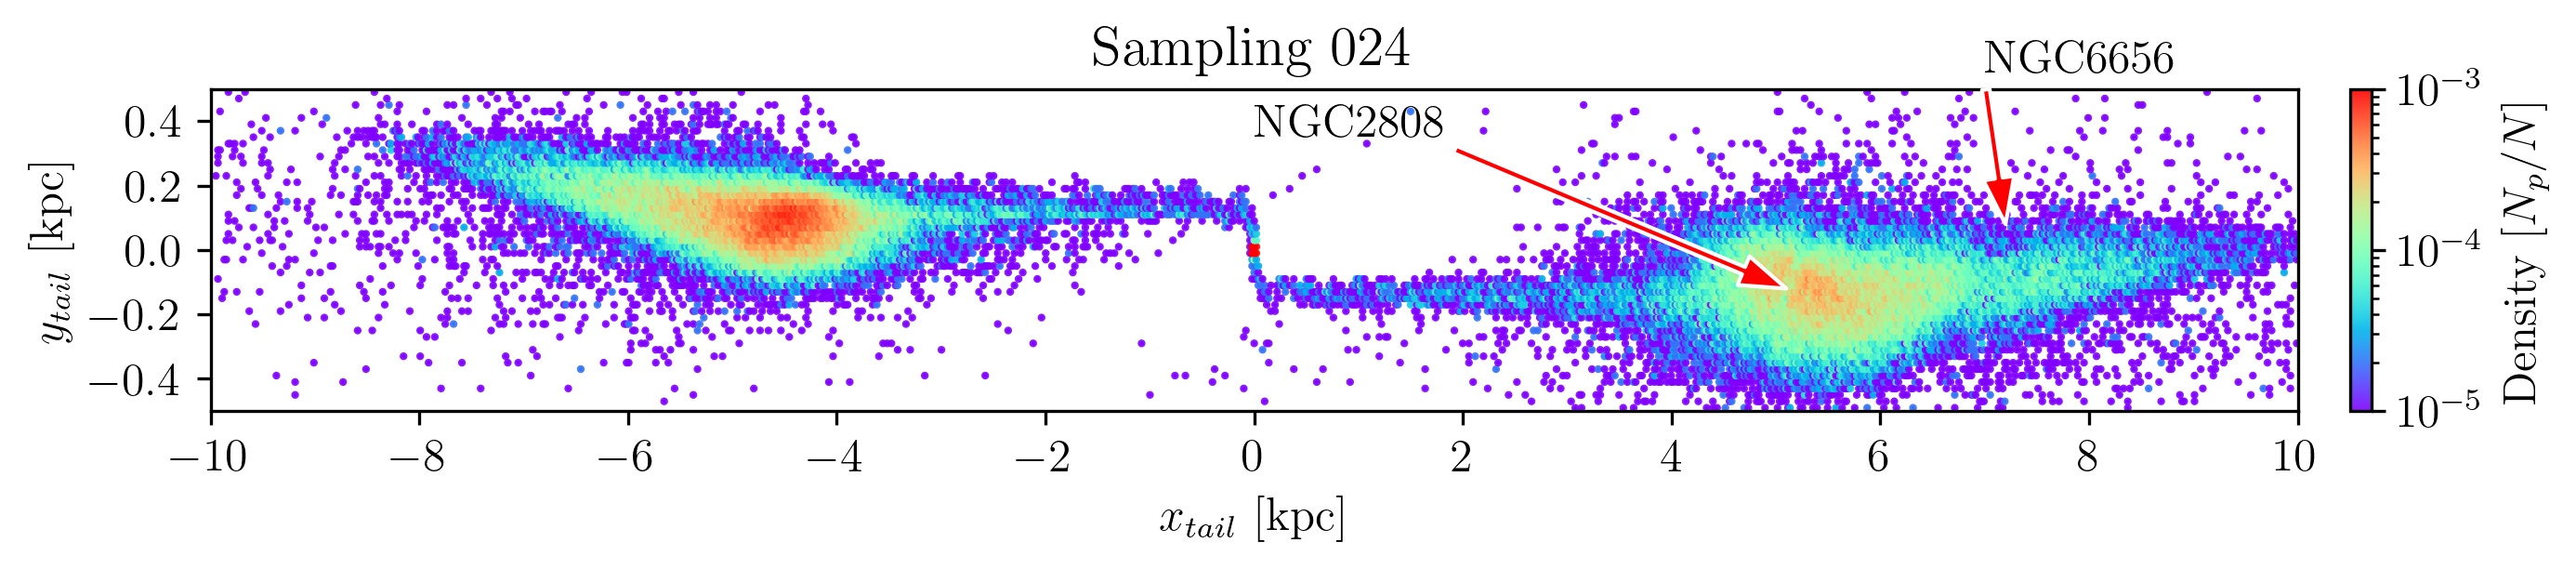
\includegraphics[width=\linewidth]{gallery_of_gaps_monte-carlo-024.png}   
      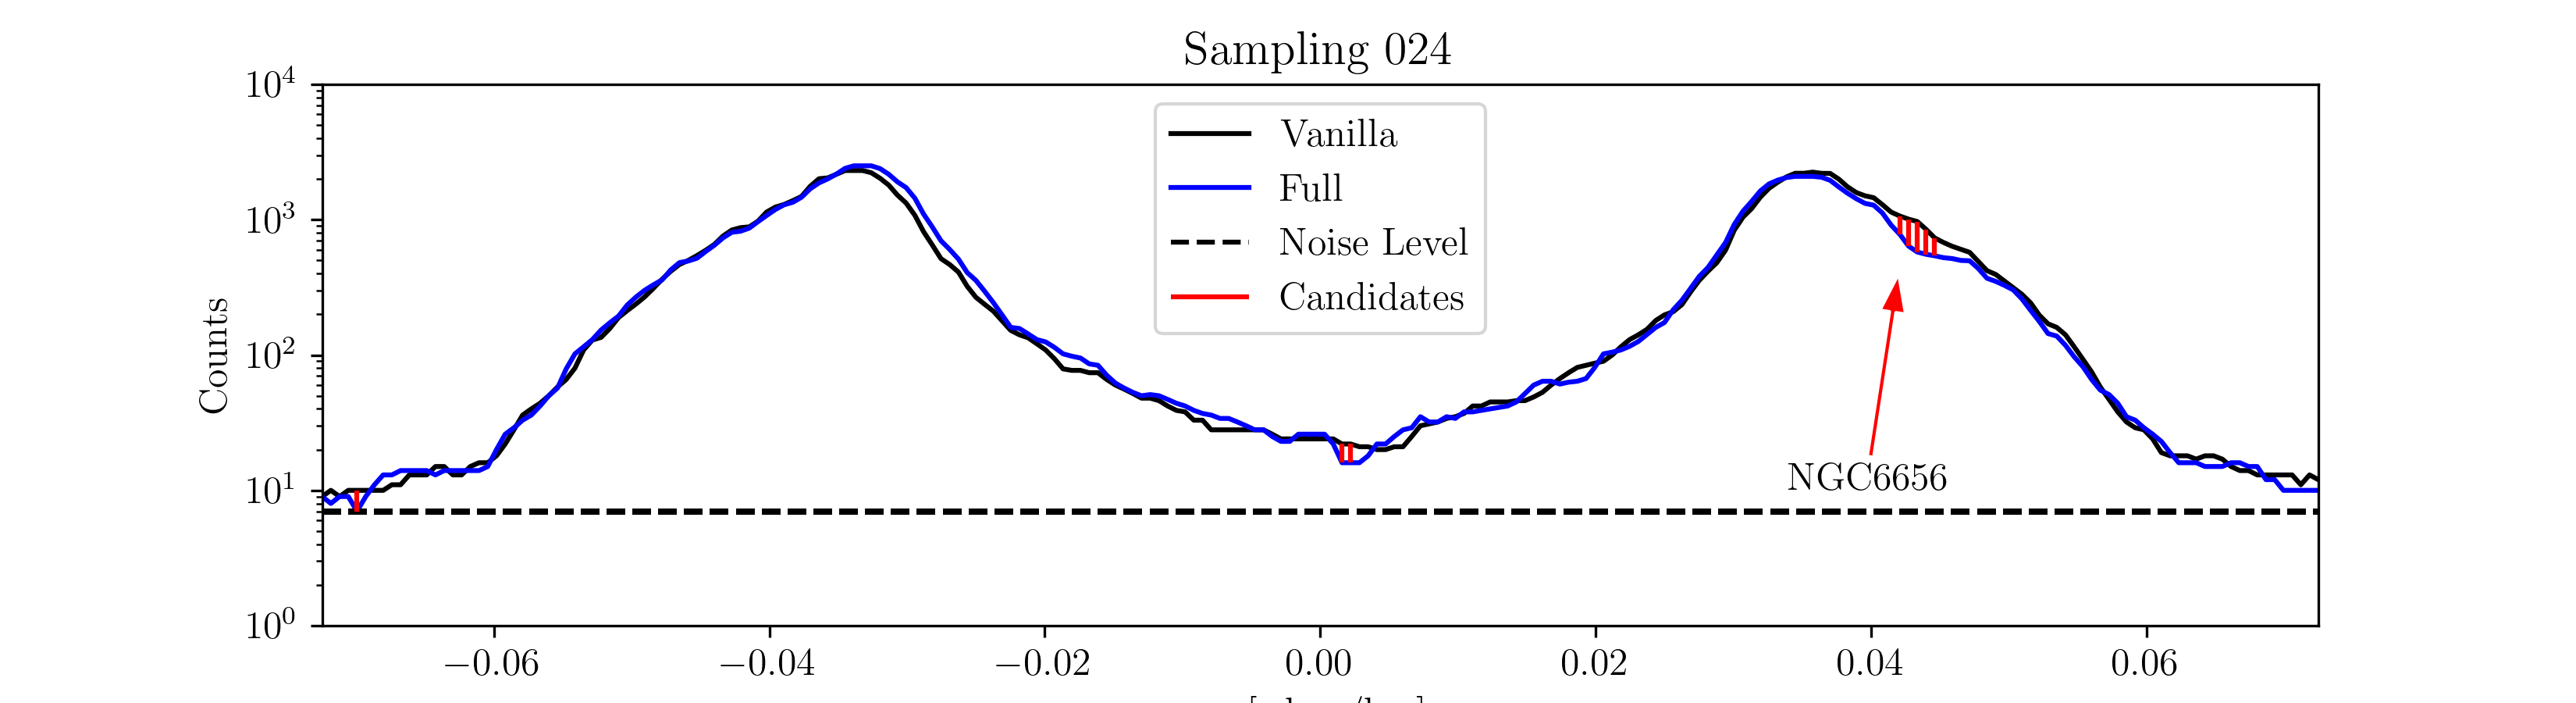
\includegraphics[width=\linewidth]{tau-profile-monte-carlo-024.png}
      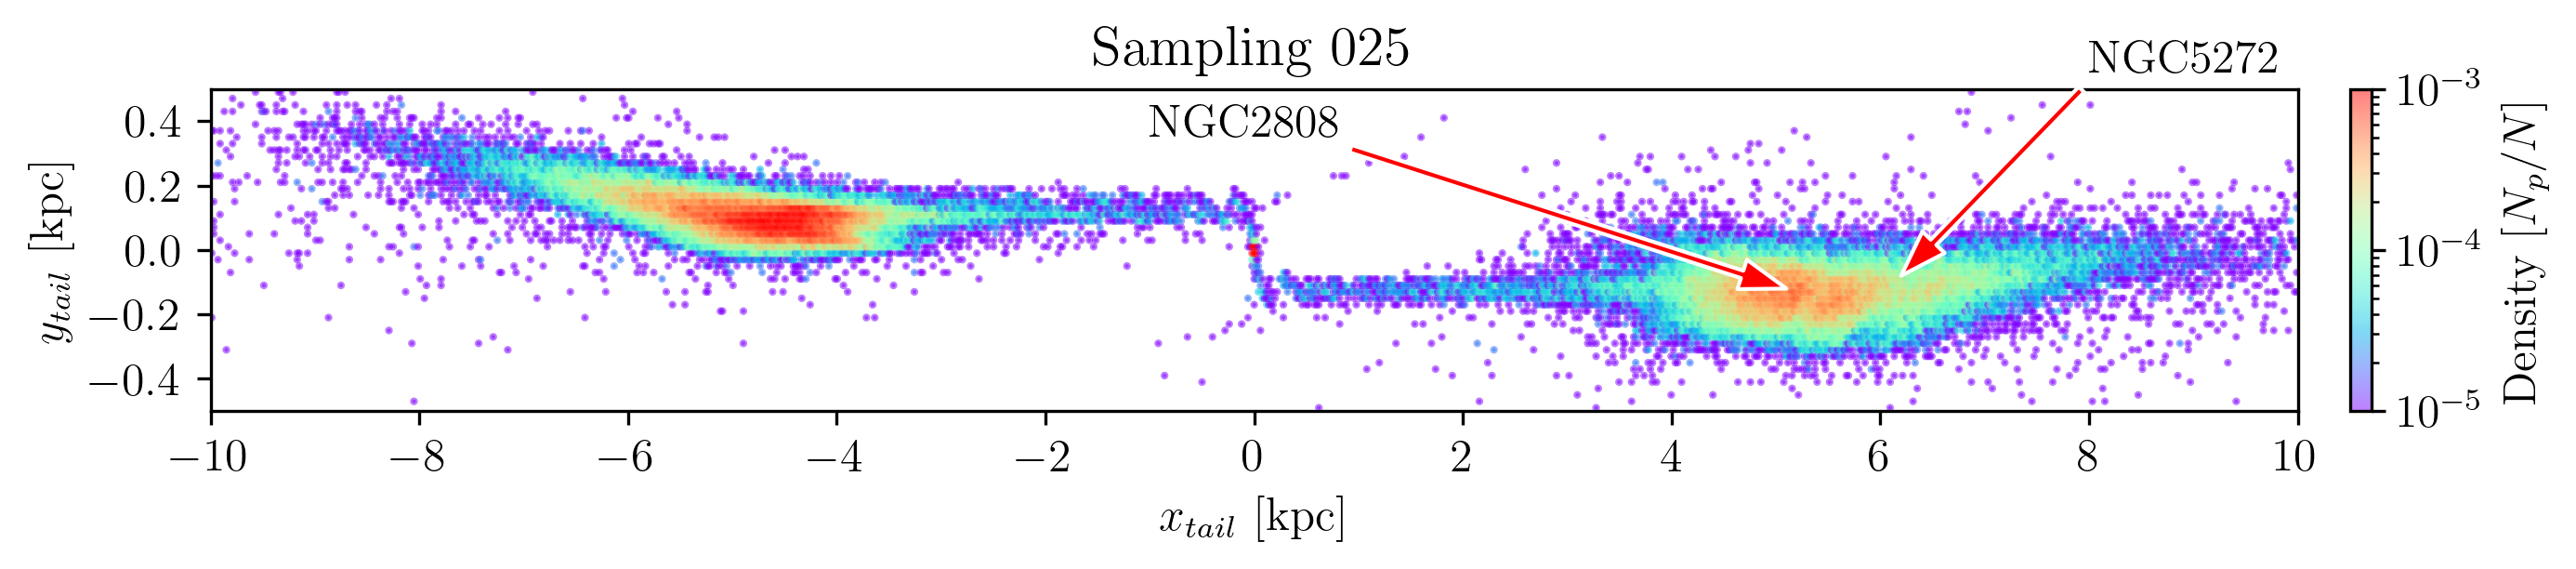
\includegraphics[width=\linewidth]{gallery_of_gaps_monte-carlo-025.png}
      \caption{Gap Gallery}
      \label{fig:gallery5}
      \end{figure*}        

    \begin{figure*}
      \centering
      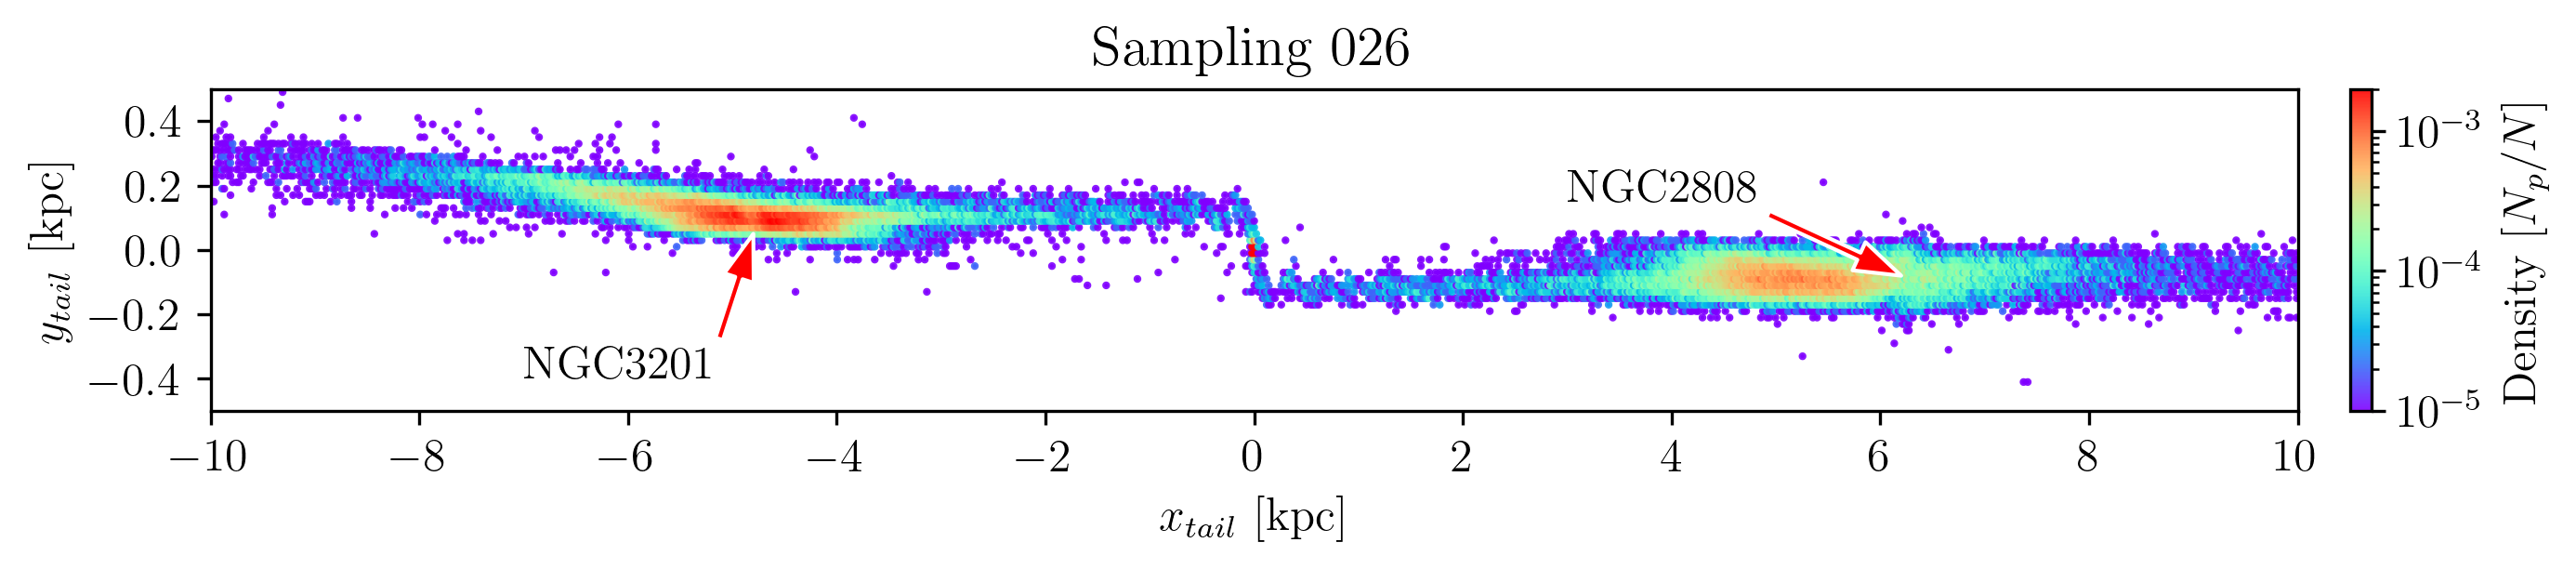
\includegraphics[width=\linewidth]{gallery_of_gaps_monte-carlo-026.png}
      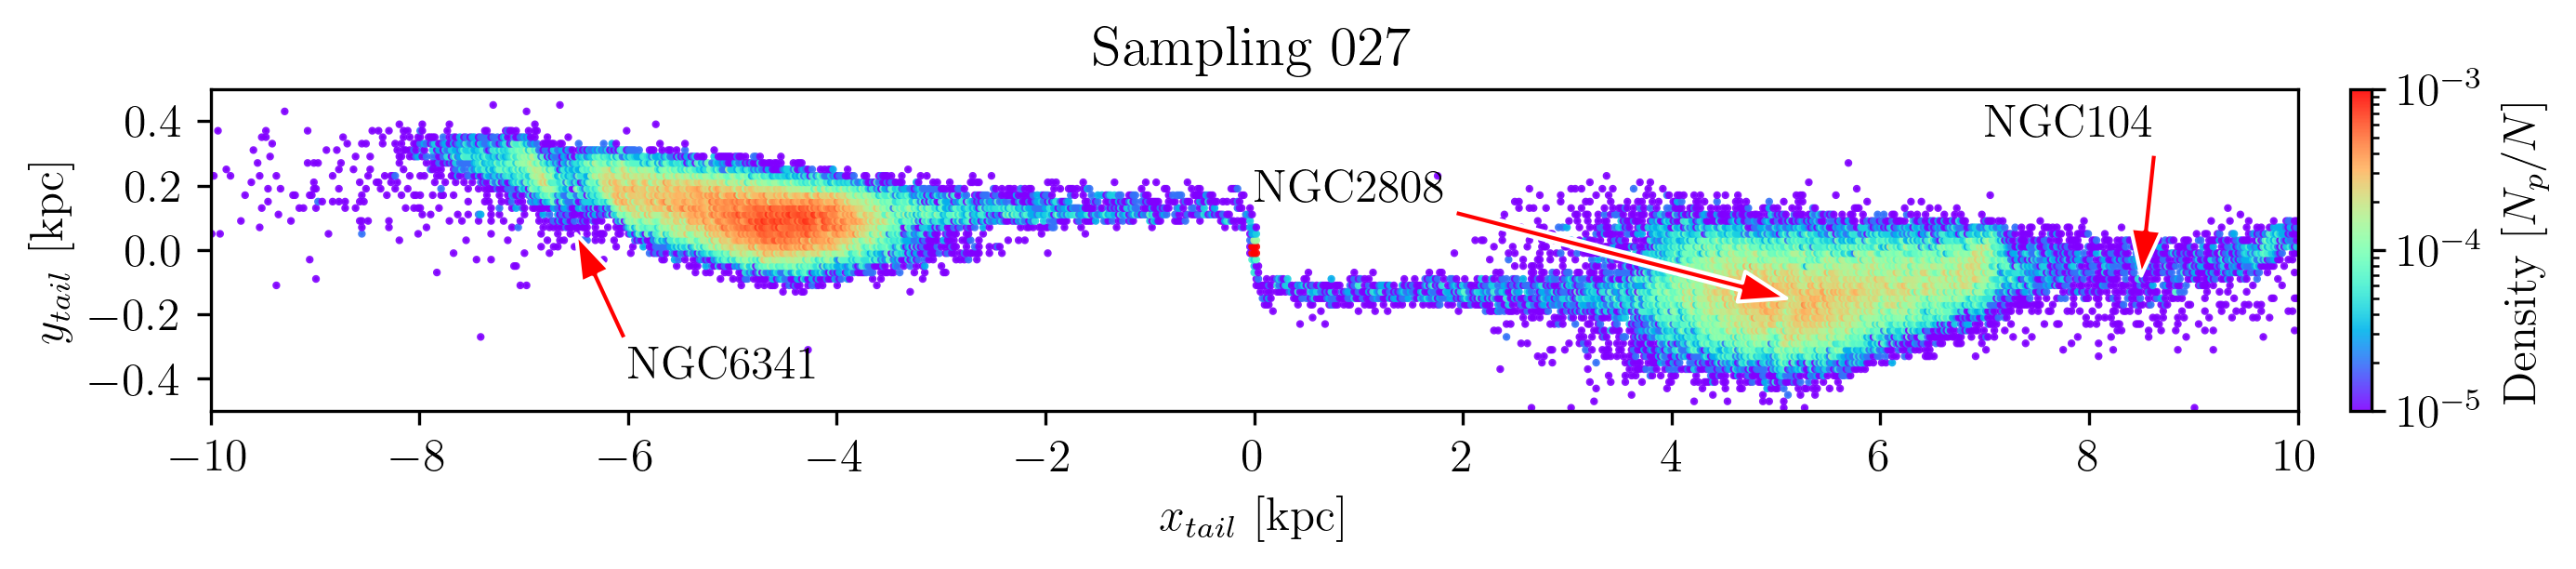
\includegraphics[width=\linewidth]{gallery_of_gaps_monte-carlo-027.png}
      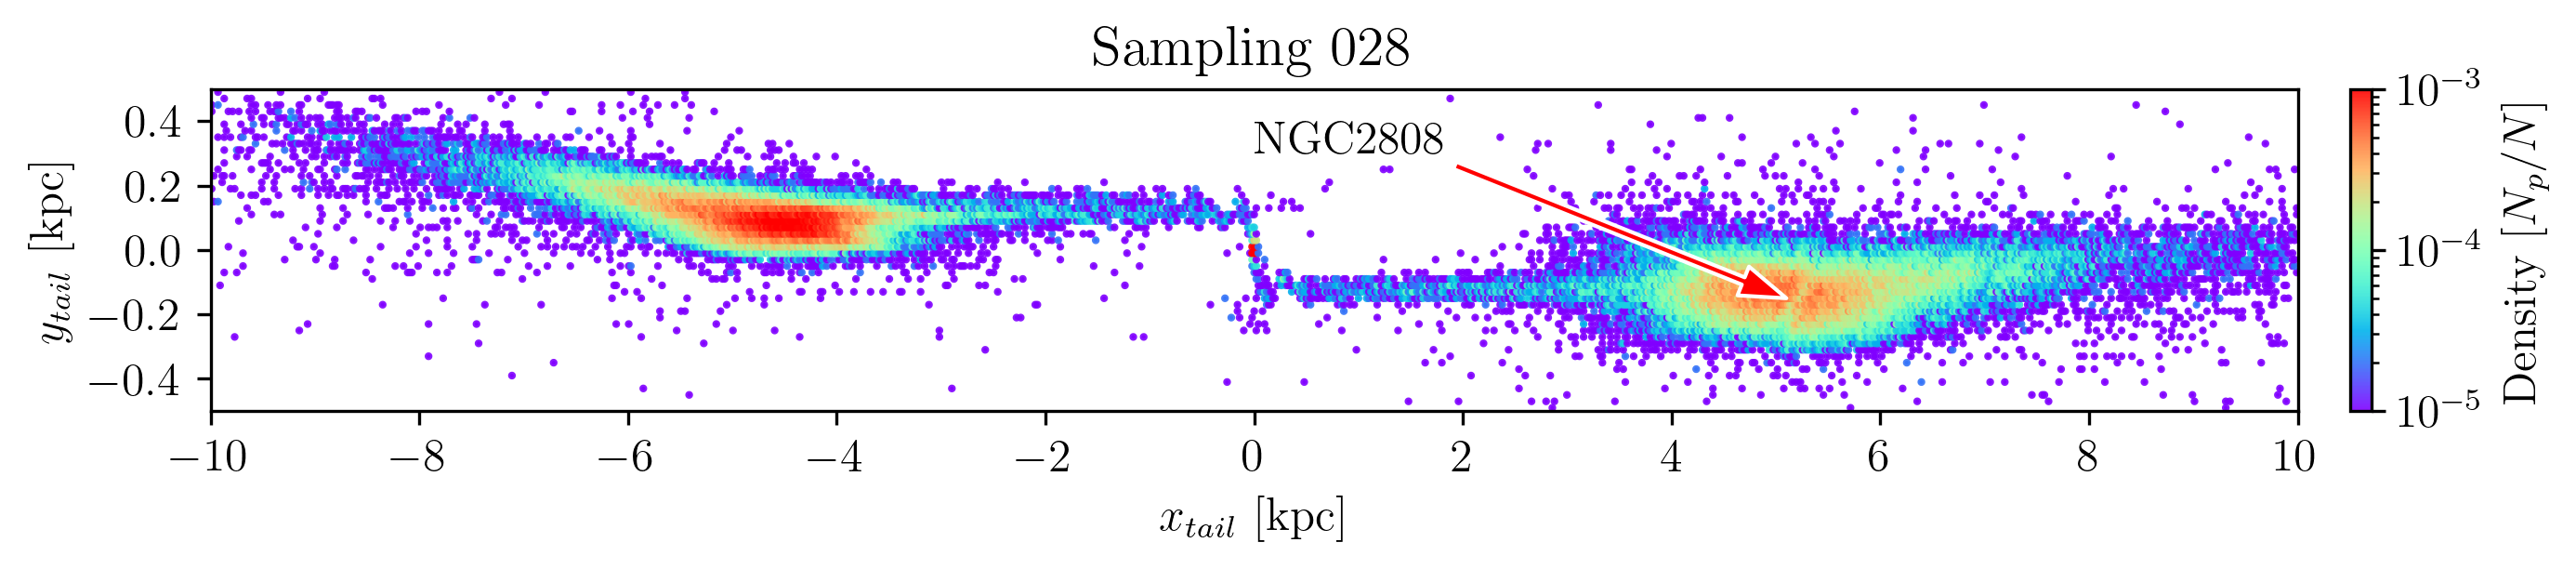
\includegraphics[width=\linewidth]{gallery_of_gaps_monte-carlo-028.png}
      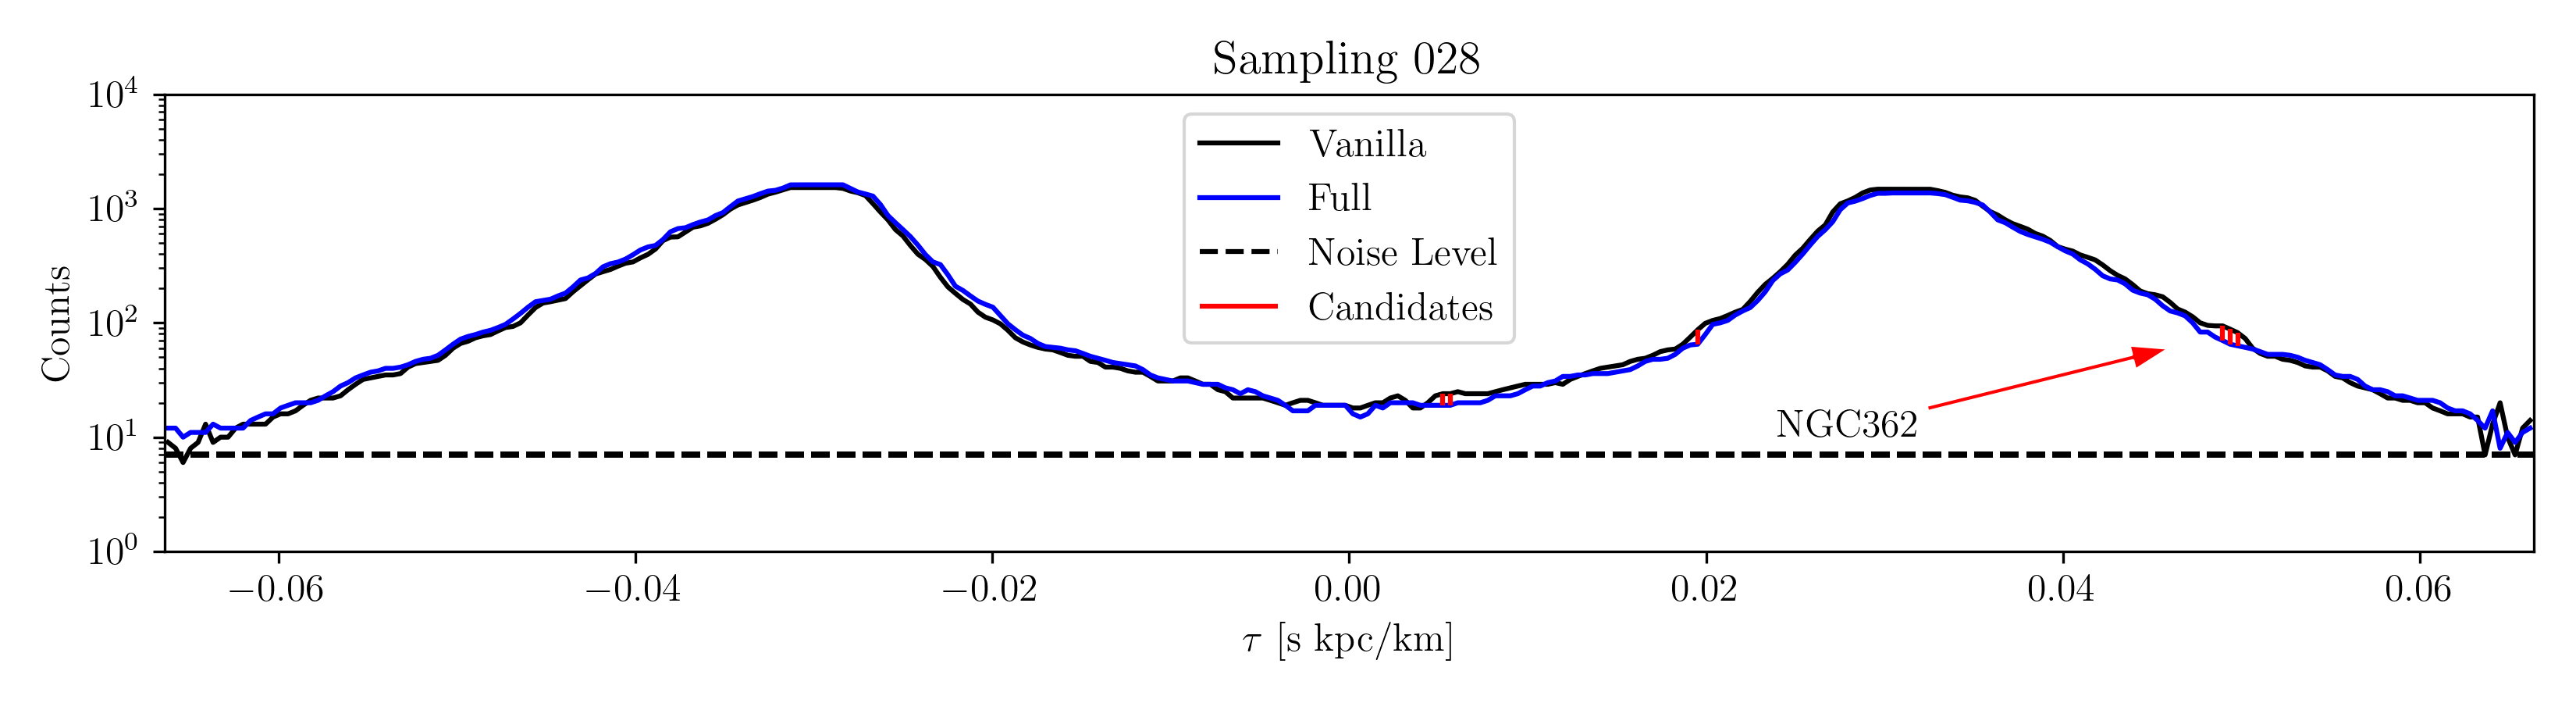
\includegraphics[width=\linewidth]{tau-profile-monte-carlo-028.png}
      \caption{Gap Gallery}
      \label{fig:gallery6}
      \end{figure*}        

    \begin{figure*}
      \centering      
      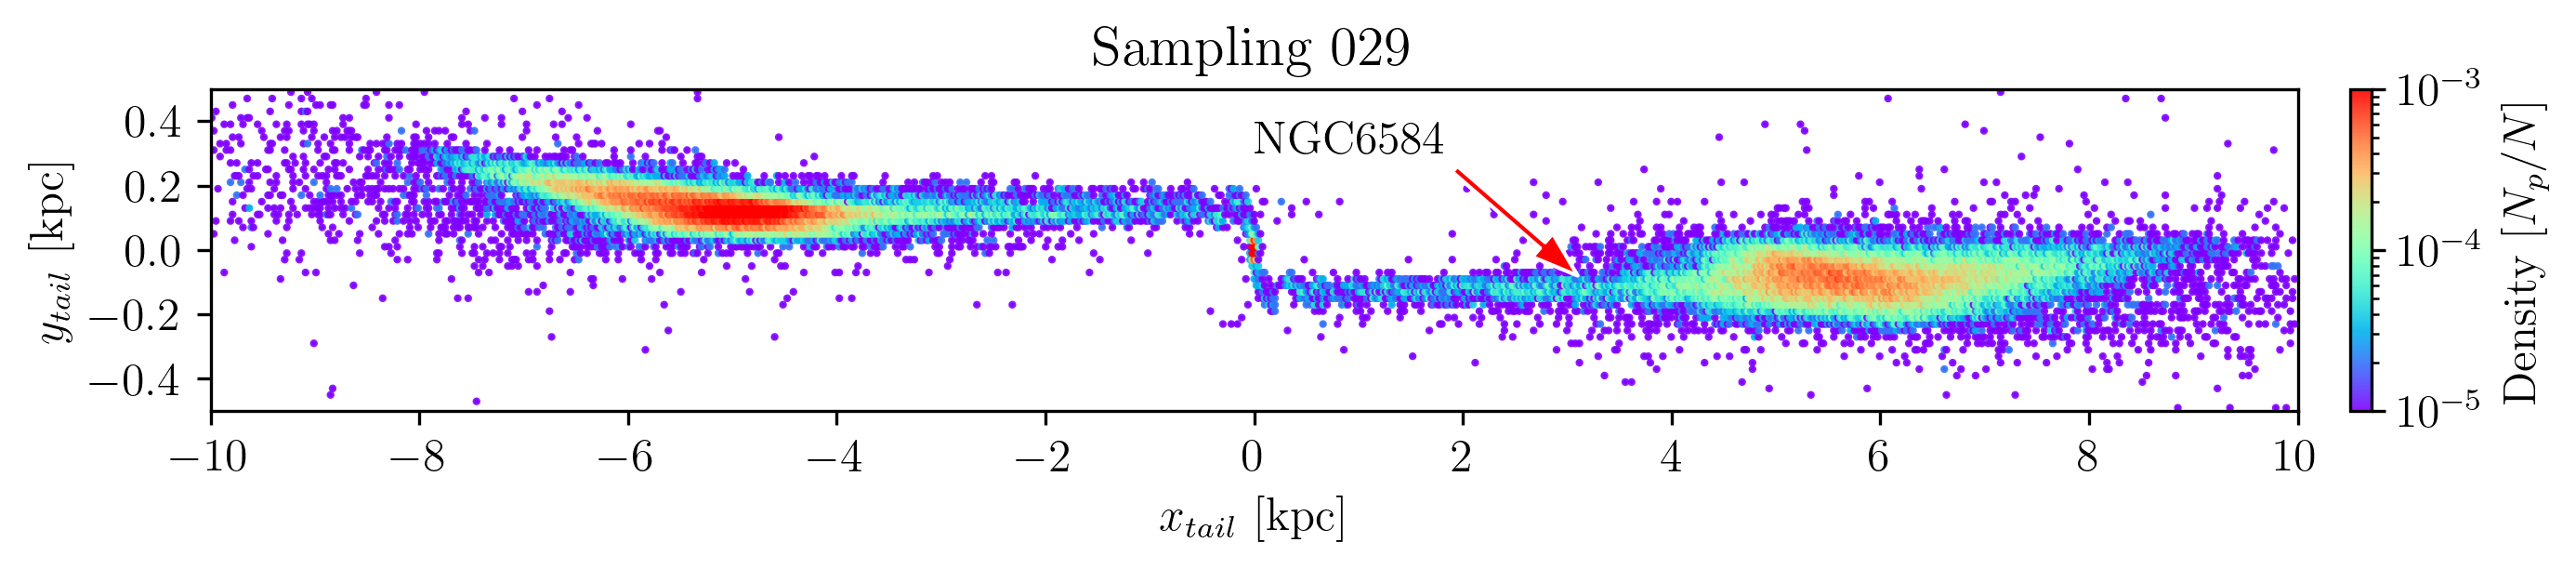
\includegraphics[width=\linewidth]{gallery_of_gaps_monte-carlo-029.png}    
      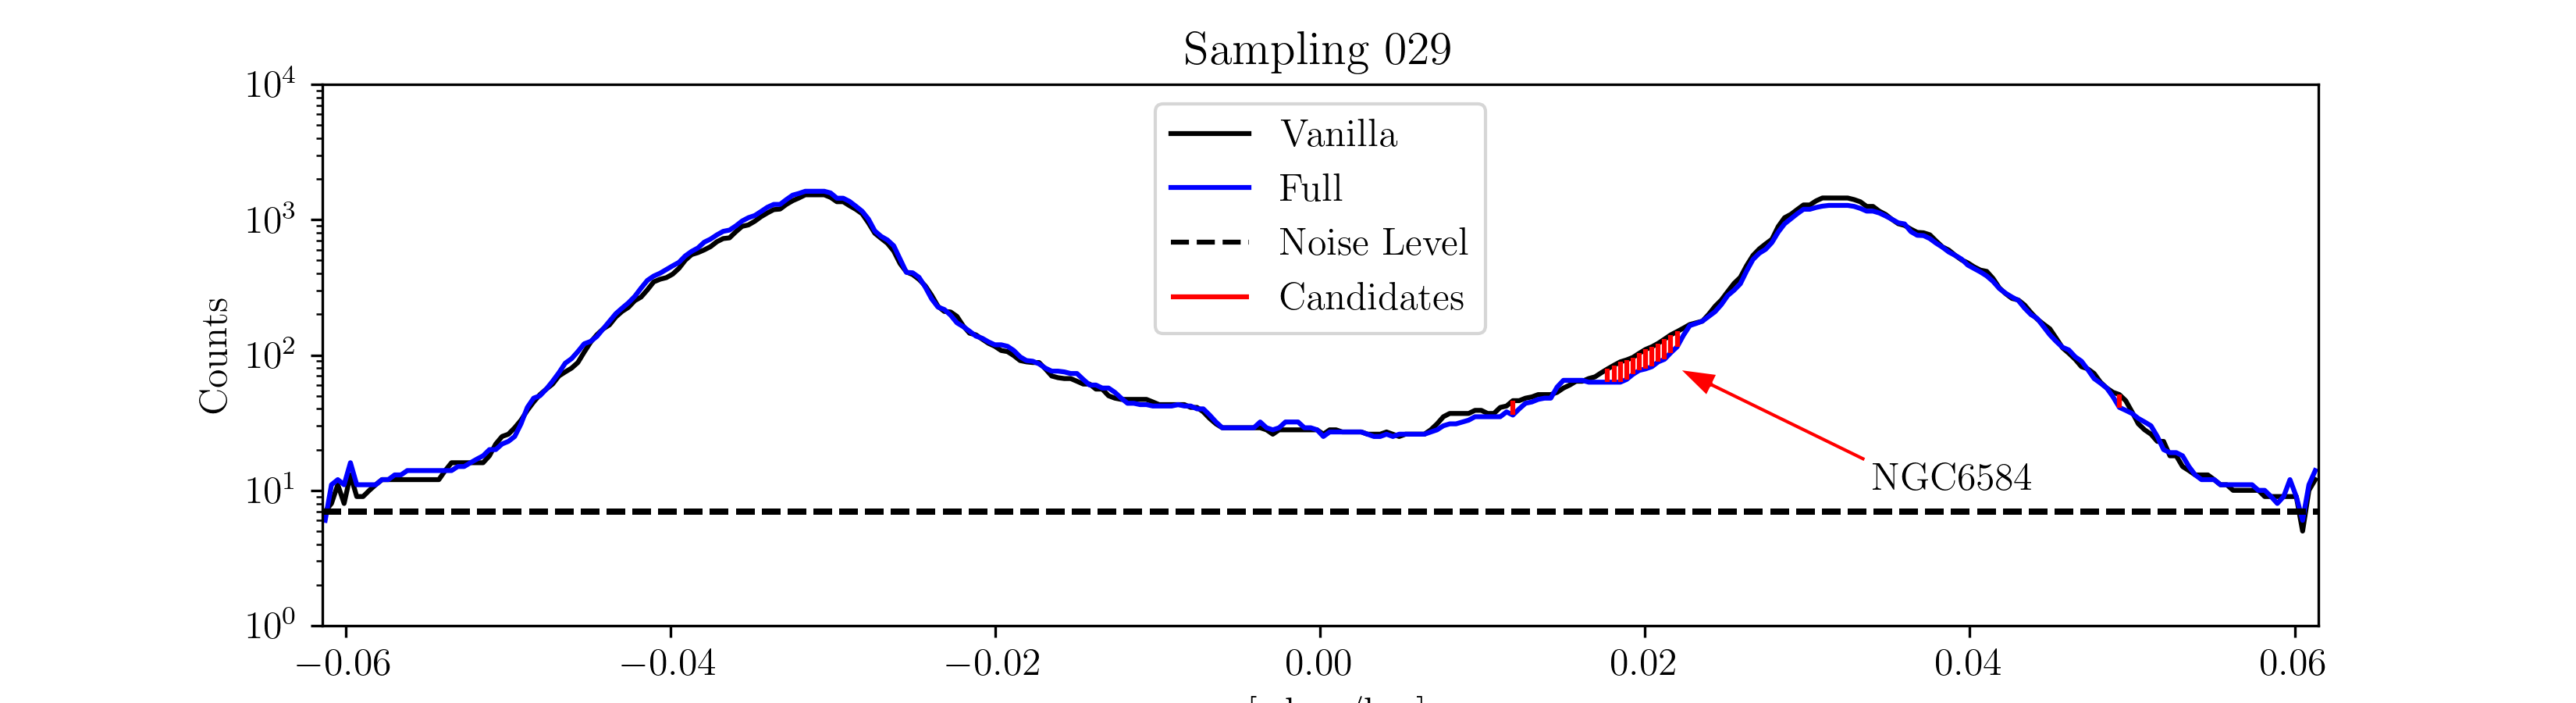
\includegraphics[width=\linewidth]{tau-profile-monte-carlo-029.png}  
      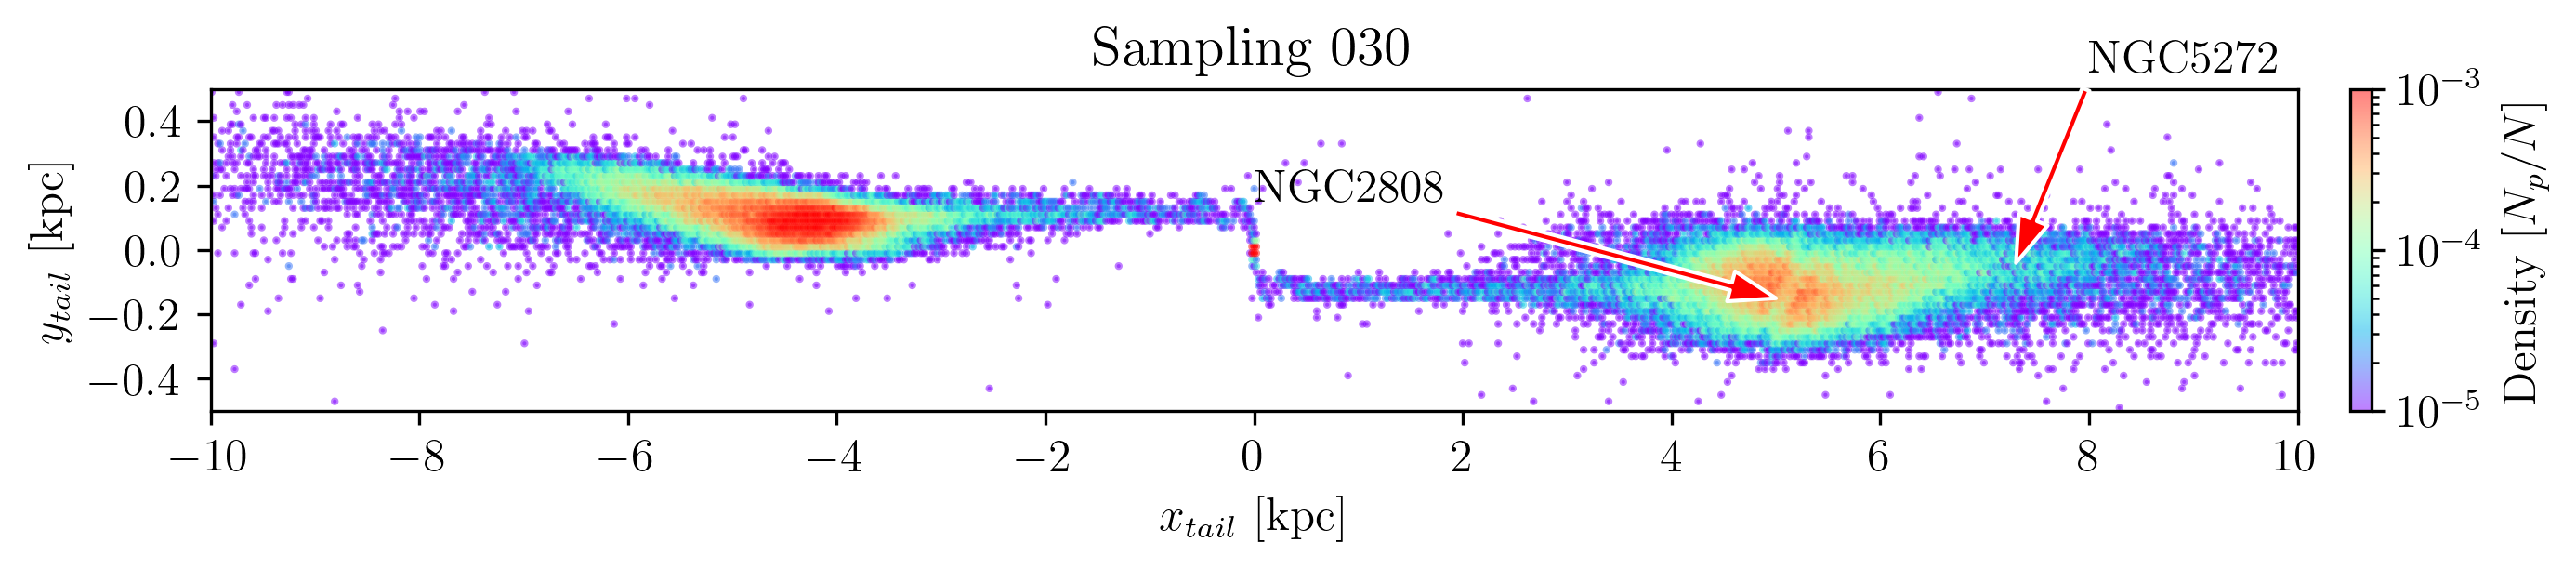
\includegraphics[width=\linewidth]{gallery_of_gaps_monte-carlo-030.png}
      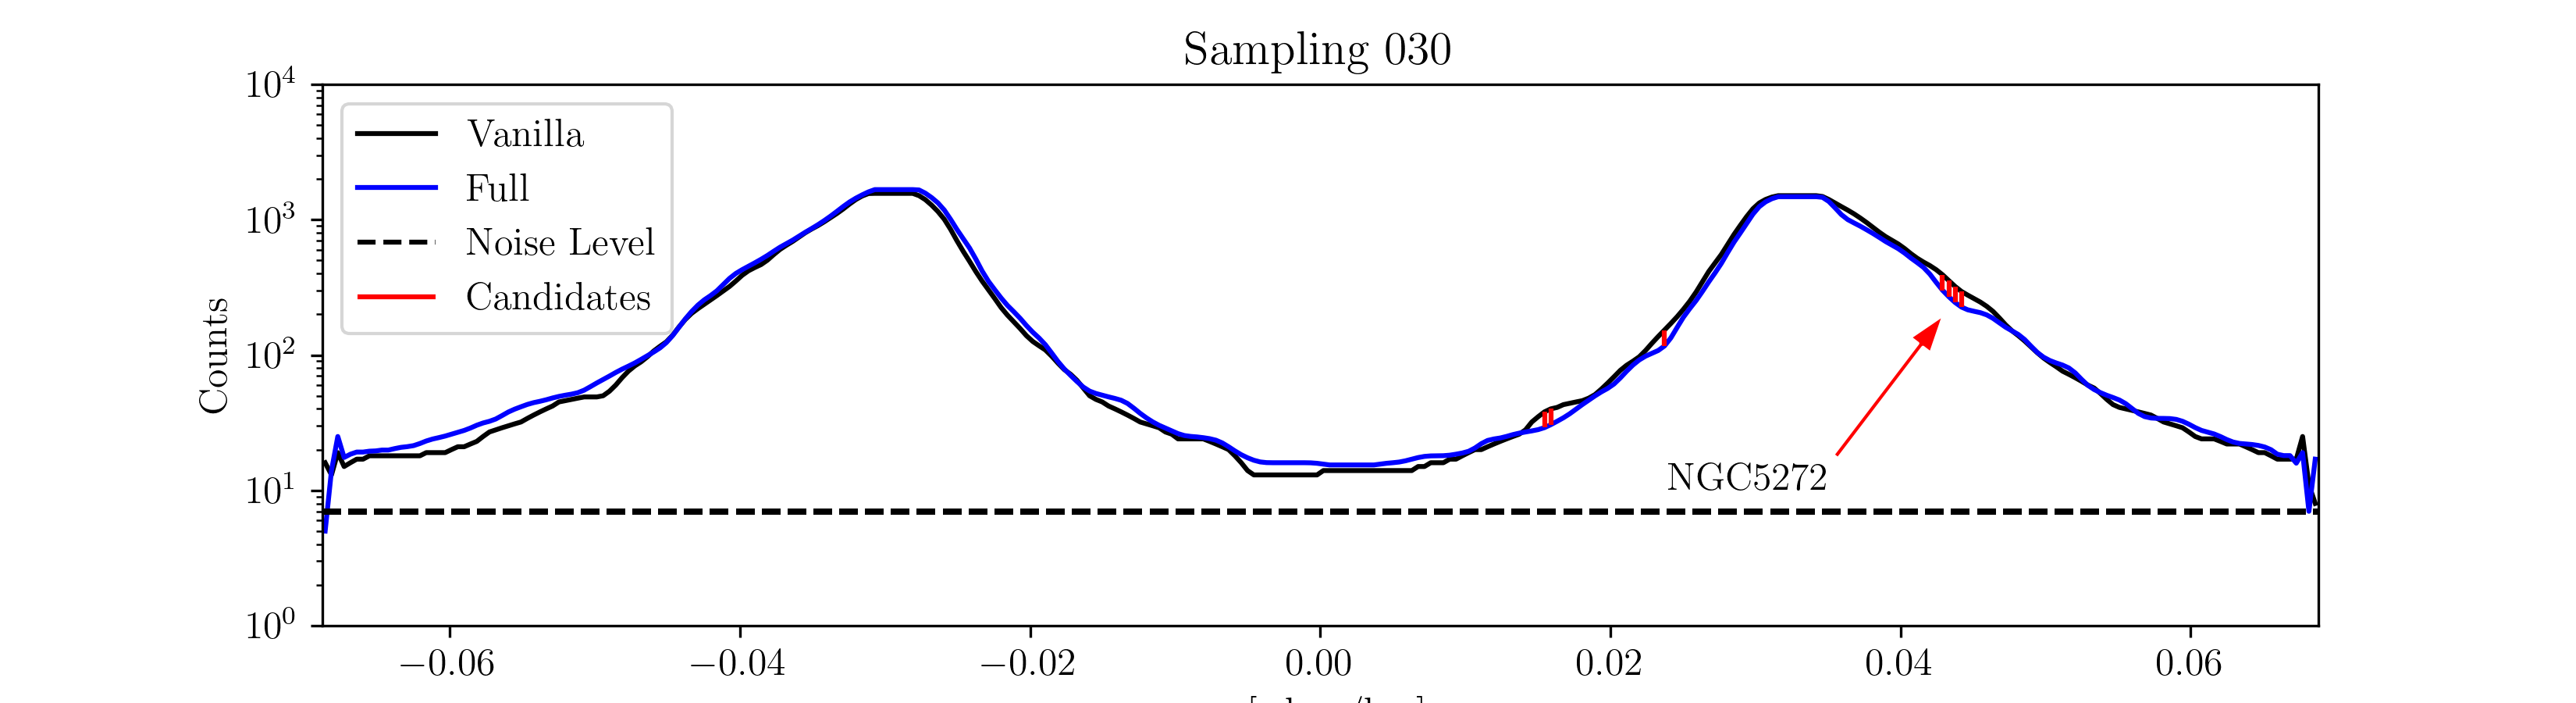
\includegraphics[width=\linewidth]{tau-profile-monte-carlo-030.png}
      \includegraphics[width=\linewidth]{gallery_of_gaps_monte-carlo-031.png}
      \caption{Gap Gallery}
      \label{fig:gallery7}
      \end{figure*}        


    \begin{figure*}
      \centering
      \includegraphics[width=\linewidth]{gallery_of_gaps_monte-carlo-032.png}
      \includegraphics[width=\linewidth]{gallery_of_gaps_monte-carlo-033.png}
      \includegraphics[width=\linewidth]{gallery_of_gaps_monte-carlo-034.png}      
      \includegraphics[width=\linewidth]{gallery_of_gaps_monte-carlo-035.png}
      \includegraphics[width=\linewidth]{gallery_of_gaps_monte-carlo-036.png}      
      \caption{Gap Gallery}
      \label{fig:gallery8}
      \end{figure*}    



    \begin{figure*}
      \centering
      \includegraphics[width=\linewidth]{gallery_of_gaps_monte-carlo-037.png}
      \includegraphics[width=\linewidth]{gallery_of_gaps_monte-carlo-038.png}
      \includegraphics[width=\linewidth]{gallery_of_gaps_monte-carlo-039.png}
      \includegraphics[width=\linewidth]{gallery_of_gaps_monte-carlo-040.png}
      \includegraphics[width=\linewidth]{gallery_of_gaps_monte-carlo-041.png}      
      \caption{Gap Gallery}
      \label{fig:gallery9}
    \end{figure*}        
    
    \begin{figure*}
      \centering
      \includegraphics[width=\linewidth]{gallery_of_gaps_monte-carlo-042.png}
      \includegraphics[width=\linewidth]{gallery_of_gaps_monte-carlo-043.png}
      \includegraphics[width=\linewidth]{gallery_of_gaps_monte-carlo-044.png}
      \includegraphics[width=\linewidth]{tau-profile-monte-carlo-044.png}
      \includegraphics[width=\linewidth]{gallery_of_gaps_monte-carlo-045.png}
      \caption{Gap Gallery}
      \label{fig:gallery010}
    \end{figure*}   

    \begin{figure*}
      \centering
      \includegraphics[width=\linewidth]{gallery_of_gaps_monte-carlo-046.png}
      \includegraphics[width=\linewidth]{gallery_of_gaps_monte-carlo-047.png}
      \includegraphics[width=\linewidth]{gallery_of_gaps_monte-carlo-048.png}
      \includegraphics[width=\linewidth]{tau-profile-monte-carlo-048.png}
      \includegraphics[width=\linewidth]{gallery_of_gaps_monte-carlo-049.png}
      \caption{Gap Gallery}
      \label{fig:gallery11}
    \end{figure*} 

\end{appendix}



\end{document}